\documentclass[12pt,a4paper]{report}

\usepackage[utf8]{inputenc}
\usepackage[T1]{fontenc}
\usepackage[english]{babel}
\usepackage[margin=2.5cm]{geometry}

\usepackage{graphicx}
\graphicspath{{assets/docs/}}
\usepackage{amsmath,amssymb}

\usepackage{array}
\usepackage{booktabs}
\usepackage{tabularx}
\usepackage{longtable}

\usepackage{float}
\usepackage{caption}
\usepackage{subcaption}
\usepackage[section]{placeins}

\usepackage{microtype}
\usepackage{enumitem}
\usepackage{listings}
\usepackage{xcolor}

\usepackage{tikz}
\usetikzlibrary{
    arrows.meta,
    positioning,
    shapes.geometric,
    fit,
    backgrounds,
    calc
}

\usepackage{url}
\usepackage{hyperref}

\hypersetup{
    colorlinks=true,
    linkcolor=blue,
    citecolor=blue,
    urlcolor=blue,
    pdftitle={IoT-SecureGate Unified Software Platform},
    pdfsubject={Bachelor Thesis Project},
    pdfkeywords={
        IoT,
        MQTT,
        authentication,
        intrusion detection,
        gateway management,
        monitoring,
        IoT-SecureGate
    }
}

\setcounter{secnumdepth}{2}
\setcounter{tocdepth}{2}

\setlength{\parindent}{0pt}
\setlength{\parskip}{6pt}
\setlength{\emergencystretch}{3em}

\renewcommand{\arraystretch}{1.2}
\urlstyle{same}

\setlist[itemize,1]{
    label=\textbullet,
    leftmargin=2em,
    labelsep=0.5em,
    itemindent=0pt,
    listparindent=0pt,
    topsep=6pt,
    itemsep=6pt,
    parsep=0pt,
    partopsep=0pt
}

\setlist[itemize,2]{
    label=\textendash,
    leftmargin=1.8em,
    labelsep=0.5em,
    itemindent=0pt,
    listparindent=0pt,
    topsep=3pt,
    itemsep=3pt,
    parsep=0pt,
    partopsep=0pt
}

\setlist[enumerate]{
    leftmargin=2em,
    labelsep=0.5em,
    itemindent=0pt,
    listparindent=0pt,
    topsep=6pt,
    itemsep=4pt,
    parsep=0pt,
    partopsep=0pt
}

\newcolumntype{Y}{
    >{\raggedright\arraybackslash}X
}

\newcolumntype{P}[1]{
    >{\raggedright\arraybackslash}p{#1}
}

\definecolor{codebackground}{rgb}{0.96,0.96,0.96}

\lstset{
    basicstyle=\ttfamily\small,
    backgroundcolor=\color{codebackground},
    breaklines=true,
    frame=single,
    columns=fullflexible,
    keepspaces=true,
    showstringspaces=false,
    captionpos=b,
    tabsize=4
}

\tikzset{
    box/.style={
        draw,
        rounded corners,
        align=center,
        text width=10cm,
        minimum height=9mm,
        font=\small
    },
    flow/.style={
        -{Latex[length=2mm]},
        thick
    },
    archbox/.style={
        draw,
        rounded corners=2pt,
        align=center,
        font=\scriptsize\sffamily,
        inner sep=4pt,
        minimum height=8mm
    },
    archcomp/.style={
        archbox,
        fill=gray!8,
        text width=2.5cm
    },
    archhost/.style={
        draw,
        dashed,
        rounded corners=3pt,
        inner sep=8pt,
        align=center,
        font=\small\sffamily\bfseries
    },
    archlabel/.style={
        font=\scriptsize\sffamily,
        align=center
    },
    archflow/.style={
        -{Latex[length=1.8mm]},
        thick,
        font=\scriptsize\sffamily
    },
    archflowsoft/.style={
        -{Latex[length=1.8mm]},
        thick,
        dashed,
        font=\scriptsize\sffamily
    }
}

% Screenshots from assets/docs/
\newcommand{\appshot}[4][]{%
    \begin{figure}[htbp]
        \centering
        \IfFileExists{#2}{%
            \includegraphics[
                width=0.96\linewidth,
                height=0.68\textheight,
                keepaspectratio
            ]{#2}%
        }{%
            \fbox{%
                \parbox{0.88\linewidth}{%
                    \centering
                    \vspace{0.4cm}
                    Image file not found:\\[4pt]
                    \texttt{\detokenize{#2}}\\[6pt]
                    Place the file under \texttt{assets/docs/}.
                    \vspace{0.4cm}
                }%
            }%
        }%
        \caption[#3]{#3.}%
        \label{#4}%
    \end{figure}%
}

\newcommand{\ReportHeading}{
    IoT-SecureGate: Unified Software Platform
    for Secure Edge IoT Gateways
}

\newcommand{\SubmissionYear}{2026}

\begin{document}

% =========================================================
% TITLE PAGE — shared project team
% =========================================================
\begin{titlepage}
    \centering

    \noindent
    \begin{minipage}{\textwidth}
        \raggedright

        \IfFileExists{VGU-Logo.png}{
            
\includegraphics[width=4cm]{VGU-Logo.png}
        }{
            \vspace*{1cm}
        }
    \end{minipage}

    \vspace{0.8cm}

    {\large Vietnamese-German University\par}

    \vspace{0.15cm}

    {\large
        Electrical and Computer Engineering Study Program
        \par
    }

    \vfill

    {\huge\bfseries BACHELOR THESIS \par}

    {\huge\bfseries Title:\par}

    \vspace{0.4cm}

    {\Large\bfseries \ReportHeading\par}

    \vspace{0.4cm}


    \vfill

    {\large By\par}

    \vspace{0.4cm}

    \begin{tabular}{lc}
        \toprule
        \textbf{Name} & \textbf{Student ID} \\
        \midrule
        Nguyen Tran Son Tung & 10222035 \\
        Nguyen Minh Bach     & 10222002 \\
        Pham Huynh Tri Thuc  & 10222058 \\
        \bottomrule
    \end{tabular}

    \vspace{0.8cm}

    \begin{tabular}{ll}
        First Supervisor:
        & Assoc. Prof. Dr. Chan Thai Truyen Dai \\[0.2cm]

        Second Supervisor:
        & Mr. Tran Quang Nhu \\
    \end{tabular}

    \vfill

    

    \vfill

    {\large
        Vietnamese-German University, \SubmissionYear
        \par
    }
\end{titlepage}

% =========================================================
% FRONT MATTER
% =========================================================
\pagenumbering{roman}

\begin{abstract}

In manufacturing and other factory-floor IoT deployments, edge sensors
continuously send measurements into internal systems that drive monitoring,
control, and production decisions. Those edge devices sit outside the trusted
core of the plant network, so unauthorized clients, stolen credentials, or
malicious publishers can inject false data or abuse messaging channels.
Without a controlled entry point, the plant cannot reliably decide which
devices may speak, what they may publish, or when a source should be cut off.

IoT-SecureGate is a security gateway for this setting. It sits between edge
devices and the internal network and gives administrators a single place to
govern incoming sensor messages, monitor the gateway and data path through
operational metrics, and detect denied or invalid traffic so misuse can be
stopped. The platform authenticates and authorizes devices before they may
publish, protects inbound transmission, keeps the health of that path
visible, and supports operator response when traffic is denied or abnormal.

This thesis presents the design and implementation of that secure gateway.
Relative to earlier research prototypes, the work also delivers the gateway
as a ready-to-use software package for operators. The report evaluates the
gateway functions in operation and notes directions in which the system can
be improved in future work.

\medskip
\noindent
\textbf{Keywords:}
IoT security, edge gateway, MQTT, device authentication,
manufacturing IoT, gateway monitoring.

\end{abstract}

\chapter*{Acknowledgements}
\phantomsection
\addcontentsline{toc}{chapter}{Acknowledgements}

We would like to thank our supervisors for their guidance, feedback, and support throughout this project.
We also thank the academic staff who provided advice during the development and preparation of this thesis.


\tableofcontents
\listoffigures
\listoftables

\clearpage

\chapter*{Abbreviations}
\phantomsection
\addcontentsline{toc}{chapter}{Abbreviations}

\begin{tabularx}{\textwidth}{|P{2.5cm}|Y|}
    \hline
    \textbf{Term} & \textbf{Meaning} \\
    \hline
    ACL & Access Control List \\
    \hline
    API & Application Programming Interface \\
    \hline
    CA & Certificate Authority \\
    \hline
    CPU & Central Processing Unit \\
    \hline
    CSR & Certificate Signing Request \\
    \hline
    DMEC & Daily Message Encryption Certificate \\
    \hline
    GUI & Graphical User Interface \\
    \hline
    IDS & Intrusion Detection System \\
    \hline
    IoT & Internet of Things \\
    \hline
    JSON & JavaScript Object Notation \\
    \hline
    MQTT & Message Queuing Telemetry Transport \\
    \hline
    mTLS & Mutual Transport Layer Security \\
    \hline
    PKI & Public Key Infrastructure \\
    \hline
    RAM & Random Access Memory \\
    \hline
    SSH & Secure Shell \\
    \hline
    TLS & Transport Layer Security \\
    \hline
    UI & User Interface \\
    \hline
\end{tabularx}

\clearpage
\pagenumbering{arabic}

% =========================================================
% CHAPTERS — write the platform story here
% =========================================================

\chapter{Introduction}
\label{ch:introduction}

\section{Background and Motivation}

Modern manufacturing and factory environments rely on
Internet of Things (IoT) edge devices---sensors on
machines, lines, and cells---to stream measurements into
internal monitoring and control systems. That inbound
telemetry supports production visibility, quality checks,
and operational decisions. The communication pattern is
typically publish/subscribe over MQTT: many constrained
clients send data through a broker toward applications
inside the plant~\cite{mqtt}.

The edge is also an exposed surface. Devices may be
physically accessible, credentials may leak, and a
compromised or spoofed publisher can inject false readings
or abuse messaging channels that reach systems behind the
plant boundary. As factories connect more sensors, the
risk is no longer limited to a single host: an untrusted
edge client that can publish freely becomes a path into
the internal data path that operators and receivers depend
on.

A security gateway is therefore required at the boundary
between edge devices and the internal network. Its job is
to decide which devices may transmit, under which
identity and topic policy, with which cryptographic
protections, and to keep that inbound path observable so
that misuse can be detected and stopped. IoT-SecureGate
is developed for that role: a secure edge gateway that
authenticates devices, controls transmission into the
plant side, protects message content, and supports
operator response when traffic is denied or invalid.

\section{Problem Statement}

Without a dedicated gateway, factory IoT traffic often
arrives through a broker that accepts clients with weak
or manually maintained credentials, little binding between
device identity and allowed topics, and limited visibility
into failed or abusive publishes. Operators then face
three concrete failures:

\begin{itemize}
    \item \textbf{Uncontrolled admission.}
    Unknown or poorly identified devices can reach the
    broker and publish toward internal consumers.
    \item \textbf{Unprotected or weakly protected
    transmission.}
    Payloads may travel without mutual authentication,
    without application-layer confidentiality after TLS
    termination, or without checks that the message shape
    matches what the gateway expects.
    \item \textbf{Weak response to misuse.}
    Denied connections and invalid messages may leave only
    raw broker logs, with no clear path to alert the
    operator, revoke publish rights, or quarantine a
    hostile source.
\end{itemize}

The central problem of this thesis is how to operate a
secure gateway end to end for such environments: admit
only registered edge devices, enforce authentication and
authorization on the path into the internal network,
protect and validate messages, observe gateway and message
activity, and restrict devices that violate policy.

\section{Project Aim and Objectives}

The aim is to design, implement, and evaluate
IoT-SecureGate as one secure gateway system that governs
edge device access and inbound data transmission for
factory and similar IoT deployments. The thesis describes
that system as a whole: the operator monitoring
application and the gateway that admits, protects,
observes, and responds on the inbound sensor path.

The concrete objectives follow that function:

\begin{itemize}
    \item \textbf{Objective 1: Secure device admission.}
    Ensure that only registered devices with valid
    credentials and certificates can connect and publish
    on allowed topics.

    \item \textbf{Objective 2: Controlled and protected
    transmission.}
    Carry inbound sensor data over MQTTS, decrypt and
    validate envelopes on the gateway, and forward
    accepted data onto the internal storage and messaging
    path.

    \item \textbf{Objective 3: Monitor gateway metrics and
    transmission activity.}
    Observe the health and metrics of the gateway and the live behaviour of inbound
    transmission flows for analysis.

    \item \textbf{Objective 4: Alert and automatically
    restrict invalid sensors.}
    Detect denied and invalid messages, alert the
    administrator when such traffic appears, and provide
    mechanisms that can automatically block invalid sensors,
    with manual controls when the operator needs to intervene.
\end{itemize}

Building on earlier Senior Project prototypes, this work
also delivers the gateway as a ready-to-use software
package (desktop operator application and gateway agent)
so that the security functions above can be deployed and
operated without reconstructing the system from separate
research scripts.

\section{Report Organization}

\begin{table}[H]
\centering
\begin{tabularx}{\textwidth}{|c|Y|Y|}
\hline
\textbf{Ch.} & \textbf{Title} & \textbf{Content} \\
\hline
\ref{ch:background}
& Technical Background and Related Work
& Messaging, transport security, message protection,
  monitoring building blocks, and related research. \\
\hline
\ref{ch:requirements}
& System Requirements
& Operational context, functional and non-functional
  requirements, scope, and threat boundaries. \\
\hline
\ref{ch:architecture}
& General System Architecture
& System overview diagrams: two runtimes, planes,
  inbound path, protection layers, ports, and trust
  material. \\
\hline
\ref{ch:monitoring}
& Monitoring Application
& Operator runtime architecture, interaction with the
  gateway, and operational workflows. \\
\hline
\ref{ch:gateway}
& Gateway
& Edge runtime architecture, agent and MQTT handling,
  gateway APIs, and detection and response. \\
\hline
\ref{ch:encryption}
& Encryption and Decryption
& Transport and application-layer message protection
  workflows on the inbound path. \\
\hline
\ref{ch:evaluation}
& Evaluation
& Assessment of the system in operation. \\
\hline
\ref{ch:conclusion}
& Conclusion and Future Work
& Summary of the work and directions for later
  improvement. \\
\hline
\end{tabularx}
\caption{Organization of the report.}
\label{tab:report-organization}
\end{table}

% =========================================================
% CHAPTERS — system as a whole (not role-split modules)
% Source of truth: docs/AI-PLATFORM-KNOWLEDGE.md,
% docs/architecture.md, docs/details.md
% =========================================================

\chapter{Technical Background and Related Work}
\label{ch:background}

This chapter introduces the technical ideas needed to
read the system design that follows. It covers edge
messaging with MQTT, transport authentication with
mutual TLS, application-layer message protection,
and operational metrics and logs. A short related-work
section places the project next to common practice in
secure MQTT brokers and edge monitoring.
Implementation of IoT-SecureGate begins in later
chapters.

\section{MQTT and Edge Messaging}

MQTT is a lightweight publish/subscribe messaging
protocol widely used for IoT telemetry~\cite{mqtt}.
Clients do not send data directly to every consumer.
They connect to a \emph{broker}, which accepts
\emph{publish} operations and delivers messages to
clients that have \emph{subscribed} to matching
\emph{topics}.

A topic is a hierarchical name. Authorization at
the broker decides which clients may publish or
subscribe on which topics. That decision is separate
from the network path the packets take: a client that
can open a connection is not automatically allowed to
use every topic.

In a factory or plant setting, many edge sensors publish
measurements toward applications inside the internal
network. The broker---often placed on a local
gateway---becomes the controlled meeting point for that
inbound traffic. Understanding MQTT therefore matters
for any gateway that must admit devices, restrict topic
use, and forward accepted data further inland.

\section{Transport Security and Mutual TLS}

\subsection{Confidentiality and integrity on the wire}

Without transport protection, MQTT credentials and
payloads can be observed or altered on the network.
TLS provides an encrypted and integrity-protected
channel between client and server~\cite{tls}. When MQTT
runs over TLS (commonly called MQTTS), the broker
presents a certificate so the client can verify
that it is talking to the intended endpoint.

\subsection{Mutual authentication}

Server authentication alone does not prove who the
client is. Mutual TLS (mTLS) additionally requires the
client to present an X.509 certificate that the broker
trusts~\cite{x509}. The broker then binds the TLS
identity to local policy before accepting the MQTT
session.

Password authentication at the broker is a second,
independent check. Broker software commonly offers both
checks: a username and password to establish the client,
and topic access control lists (ACLs) that allow or deny
publish and subscribe operations per
client~\cite{mqttsurvey}.
Valid passwords do not replace topic ACLs: a client may
authenticate successfully and still be denied a
forbidden topic.

The intended access decision can be stated as:

\begin{equation}
\operatorname{AccessAllowed}
=
\operatorname{Authenticated}
\land
\operatorname{Authorized}.
\end{equation}

Authentication establishes the identity claim
(password and/or client certificate). Authorization
checks the requested publish or subscribe against
policy. Both must succeed for the operation to proceed.

\subsection{Operational limits of transport security}

TLS protects data while it travels between endpoints.
After the broker terminates TLS, the application that
reads the message sees plaintext unless a further
protection layer is applied. Certificate lifecycle
(issuance, renewal, trust store configuration) also
belongs to operational security: a correct protocol
choice still fails if devices use expired or untrusted
certificates.

\section{Application-Layer Message Protection}

Application-layer protection addresses confidentiality
and integrity of the payload \emph{after} TLS
termination, and can add checks that transport alone
does not provide.

A typical pattern is an \emph{envelope}: the sensor
encrypts the measurement under a content key, wraps
that key for the gateway, and sends one or more MQTT
messages that the gateway can unwrap, decrypt, and
validate. Authenticated encryption (for example
AES-GCM) binds confidentiality to an integrity tag so
that modified ciphertext is rejected.

Two further ideas matter for a gateway that must store
or forward decoded measurements:

\begin{itemize}
    \item \textbf{Schema validation.}
    After decrypt, the gateway checks that the JSON (or
    other) payload matches the shape expected for that
    device. A cryptographically valid message can still
    be invalid for the application.
    \item \textbf{Freshness / replay resistance.}
    Encryption does not by itself prove that a message
    is new. An application may reject repeated message
    identifiers or other freshness tokens so that a
    captured envelope cannot be replayed successfully.
\end{itemize}

Transport security and application-layer protection
answer different questions. MQTTS and mTLS answer who
may connect and publish. The envelope answers whether
the measurement remains confidential beyond the TLS
hop and whether the decoded content is acceptable to
the gateway.

After a message is accepted and decoded, a gateway
typically retains it for local audit and forwards it
onto an inland messaging or storage path so plant-side
consumers can read the same measurements. The exact
technologies used by IoT-SecureGate are described in
the architecture chapters; the background point is that
admission and decrypt are not the end of the inbound
path.

\section{Metrics, Logs, and Operational Visibility}

A secure gateway that only enforces policy still leaves
operators without evidence that the path is healthy.
Operational visibility usually combines two kinds of
signal:

\begin{itemize}
    \item \textbf{Metrics} are numerical time series
    (CPU use, memory, message rates, processing delays).
    Periodic scraping of a small set of named series from
    each monitored process is the established way to
    collect them~\cite{sre}, and Prometheus is a common
    implementation of that arrangement.
    \item \textbf{Logs} are event records (accepted
    messages, denied connections, decryption failures).
    Structuring such records so that they can be searched
    and analysed is a subject of its
    own~\cite{loganalysis}, and Loki is a common system
    for aggregating and querying them.
\end{itemize}

Dashboards (for example Grafana) present metrics and
logs so that administrators can inspect gateway health
and transmission activity without reading raw service
files. For an edge gateway, useful visibility includes
both \emph{host and service health} and \emph{message-path
activity}, including signs that traffic was denied or
failed validation. Those signals are the conceptual
basis for alerting and for deciding when a misbehaving
source should be restricted.

\section{Related Work}

\subsection{Secure MQTT at the broker}

Production MQTT deployments commonly combine TLS,
broker passwords, and topic ACLs so that only known
clients can publish on allowed
channels~\cite{mqtt,mqttsurvey}. Mutual TLS extends
that model by also requiring a trusted client
certificate, which is a standard pattern for strong
device identity on the wire~\cite{tls,x509}. Many
gateways use password authentication and client
certificates together with topic ACLs, so that
transport identity and publish rights are both
checked before a measurement is accepted.

That line of practice matches the security problems
addressed later in this thesis: register a device,
bind it to credentials and certificates, and enforce
who may connect and publish at the broker. The
background here is broker-side access control and
message protection, not a machine-learning intrusion
pipeline.

\subsection{Edge monitoring with metrics and logs}

On the operations side, scraping numerical metrics and
collecting service logs is standard for keeping hosts
and pipelines visible~\cite{sre,loganalysis}. Edge
gateways use the same idea: expose health of the
broker and processing path, and retain event records
when a connection or message is rejected.

This thesis builds on that practice for gateway
metrics and transmission activity. Denied connections
and invalid messages appear as operational signals on
that path---something the administrator can see and
act on through alerts and publish restrictions.

\subsection{Position of this work}

IoT-SecureGate sits at the intersection of those two
areas: a secure MQTT gateway with explicit device
admission and message protection, plus operator
visibility into gateway health and inbound
transmission. The following chapters describe how
that system is designed and implemented.

\chapter{System Requirements}
\label{ch:requirements}

This chapter states what IoT-SecureGate must achieve as a
secure edge gateway. Requirements follow from the problem
and objectives in Chapter~\ref{ch:introduction} and from
the operational setting of factory and similar IoT
deployments. They describe the behaviour the system must
provide; architecture and implementation appear in later
chapters. Functional requirements are labelled
FR-\textit{n}; non-functional requirements are labelled
NFR-\textit{n}. Those identifiers are reused when the
design and evaluation refer back to this chapter. The
chapter also fixes the thesis scope and the security
threat boundaries that apply to those requirements.

\section{Operational Context}

IoT-SecureGate sits between edge sensors and the
internal plant network. Sensors on machines, lines, or
cells publish measurements toward applications that
operators and plant systems use for monitoring and
control. The gateway is the controlled entry point on
that inbound path: it admits devices, authenticates and
authorizes publishes, protects and validates message
content, stores accepted data for internal consumers,
and keeps the path observable so that denied or invalid
traffic can be detected and restricted.

The platform has two runtimes that operators treat as
one system:

\begin{itemize}
    \item \textbf{Monitoring application (operator PC).}
    A packaged desktop application with a local control
    service and a local observability stack
    (Loki, Prometheus, Grafana). From this application
    the administrator discovers and provisions gateways,
    registers devices, watches metrics and transmission
    activity, and applies day-to-day control actions.
    \item \textbf{Gateway (edge device).}
    An agent on a Linux edge host (for example a
    Raspberry Pi or small Ubuntu machine) together with
    an MQTTS broker and per-sensor messaging storage.
    Sensors connect here over MQTTS. The gateway
    decrypts and validates payloads, appends accepted
    data to a local log and to Kafka broker, ships logs
    to the operator stack, and exposes metrics for
    scraping.
\end{itemize}

The primary actor is the \emph{administrator}: the
person who installs the monitoring application,
provisions gateways over the local network, registers
sensors, and responds when Activities show denied or
invalid traffic. Secondary actors are \emph{edge
sensors} (real devices or laboratory fake publishers
used for testing). Internal consumers that read stored
Kafka topics or logs sit behind the gateway; they are
not operators of the security controls themselves.

The intended deployment is a trusted plant or laboratory
LAN. The operator PC and the gateway communicate for
provision and day-2 actions over SSH. Sensor ingress
uses MQTTS on the gateway. Metrics and logs return to
the operator PC over HTTP on the same LAN. Routine
operation is meant for users who can run an installer
and use a graphical interface, without reconstructing
the stack from separate research scripts.

\section{Functional Requirements}

Functional requirements cover admission, protected
transmission, monitoring, detection and response, and
the operator path that makes those functions deployable.
They map to the four objectives in
Chapter~\ref{ch:introduction}: secure device admission,
controlled and protected transmission, gateway and
activity monitoring, and alert plus restriction of
invalid sensors.

\begin{longtable}{@{}p{1.6cm}p{\dimexpr\textwidth-1.6cm-4\tabcolsep\relax}@{}}
\caption{Functional requirements for IoT-SecureGate.}
\label{tab:functional-requirements}\\
\toprule
\textbf{ID} & \textbf{Requirement} \\
\midrule
\endfirsthead
\caption[]{Functional requirements for IoT-SecureGate
  (continued).}\\
\toprule
\textbf{ID} & \textbf{Requirement} \\
\midrule
\endhead
\bottomrule
\endlastfoot
FR-1
& The system shall admit only registered devices to the
  gateway broker. Registration shall bind a device
  identity to MQTT credentials, topic permissions, a
  client certificate under the gateway CA, and a
  reserved per-sensor storage topic. \\
\midrule
FR-2
& The gateway shall authenticate connecting clients with
  MQTT password verification and mutual TLS (client
  certificate required), and shall authorize publishes
  with topic ACLs so that a device may publish only on
  its allowed topics. \\
\midrule
FR-3
& Inbound sensor traffic shall use MQTTS on the gateway.
  After transport termination, the gateway shall decrypt
  application-layer envelopes (envelope v1), validate
  message shape against a registered schema, and reject
  traffic that fails those checks. \\
\midrule
FR-4
& Accepted message shall be written to a local sensor
  data log and produced to a per-device Kafka topic so
  that internal consumers and the operator observability
  path can use the data. \\
\midrule
FR-5
& The monitoring application shall discover and provision
  a gateway over SSH: install the agent, MQTTS broker
  configuration, and Kafka service; bootstrap gateway CA
  and server material; and record the gateway in a local
  registry with scrape and ship targets toward the
  operator stack. \\
\midrule
FR-6
& The administrator shall register and unregister devices
  from the monitoring application. Registration shall
  apply the admission material on the gateway (password,
  ACL, client certificate, crypto and schema files,
  Kafka topic) without requiring manual broker edits. \\
\midrule
FR-7
& The system shall expose gateway host and application
  health (agent, MQTT, decrypt, shipper, Kafka) as
  metrics scraped by the operator Prometheus instance,
  and shall present those metrics in the monitoring
  application. \\
\midrule
FR-8
& The system shall expose inbound transmission activity
  (message rates, delays, connected sensors, denied and
  invalid counts) through logs and summary APIs, and
  shall present that activity in the monitoring
  application. \\
\midrule
FR-9
& The gateway shall detect transport denials (failed
  authentication or ACL) and application-layer invalid
  messages (decrypt or schema failure), and shall make
  those events visible to the administrator as alerts in
  the monitoring application. \\
\midrule
FR-10
& The administrator shall be able to block and restore a
  device's publish rights (ACL change) from the
  monitoring application. \\
\midrule
FR-11
& The system shall support automatic restriction of a
  sensor source after a configurable count of invalid
  messages in a time window (firewall DROP of the source
  IP on the gateway), with an operator path to clear that
  quarantine. \\
\midrule
FR-12
& The system shall provide laboratory fake sensors on
  the gateway for testing admission, protected
  transmission, and misuse behaviours (including
  simulation of attack-like publish patterns) without
  requiring physical hardware for every test. \\
\midrule
FR-13
& The monitoring application shall install and run a
  local observability stack (Loki, Prometheus, Grafana)
  on the operator PC so that metrics and shipped logs
  are available without a separate monitoring deployment for routine use. \\
\midrule
FR-14
& Secrets used for gateway CA signing, day-2 privileged
  actions, and local admin functions shall be stored in
  the operator OS keyring (with a documented file
  fallback), and shall not be written into ordinary
  settings files or application logs. \\
\end{longtable}

FR-1 through FR-4 define the inbound security path on
the gateway. FR-5, FR-6, FR-13, and FR-14 define the
operator-side means to deploy and maintain that path.
FR-7 and FR-8 cover visibility. FR-9 through FR-11 cover
detection and response. FR-12 supports evaluation and
laboratory exercise of the same path. A packaged
machine-learning intrusion-detection module inside the
installer is outside these requirements; deny and
invalid-message handling, plus block and Auto prevent,
are the protection controls in scope.

\section{Non-Functional Requirements}

Non-functional requirements constrain how the functional
behaviour is delivered: who can operate the system, how
it is packaged, how resources and capacity are bounded,
and how trustworthy the operator path remains.

\begin{longtable}{@{}p{1.6cm}p{\dimexpr\textwidth-1.6cm-4\tabcolsep\relax}@{}}
\caption{Non-functional requirements for IoT-SecureGate.}
\label{tab:nonfunctional-requirements}\\
\toprule
\textbf{ID} & \textbf{Requirement} \\
\midrule
\endfirsthead
\caption[]{Non-functional requirements for IoT-SecureGate
  (continued).}\\
\toprule
\textbf{ID} & \textbf{Requirement} \\
\midrule
\endhead
\bottomrule
\endlastfoot
NFR-1
& \textbf{Usability.}
  Routine setup and day-to-day operation shall be
  possible through the packaged graphical monitoring
  application (install local monitoring, provision a
  gateway, register devices, view Metric and Activities,
  apply Control actions) without requiring the
  administrator to edit source code or maintain a
  multi-compose research stack for those tasks. \\
\midrule
NFR-2
& \textbf{Deployability.}
  The monitoring application shall be distributable as
  native packages for Windows and Linux so that the operator path can
  be installed on a PC without Docker or WSL as a
  default dependency. \\
\midrule
NFR-3
& \textbf{Gateway footprint.}
  The gateway runtime shall run as a service stack on a
  modest Linux edge host (agent, system Mosquitto,
  Kafka), suitable for small industrial or laboratory
  devices such as a Raspberry Pi--class machine. \\
\midrule
NFR-4
& \textbf{Capacity bound.}
  The number of registered sensors (real and laboratory
  fake) shall be limited by gateway disk budget for
  Kafka topic retention so that registration fails
  clearly when capacity is exhausted rather than filling
  the device unbounded. \\
\midrule
NFR-5
& \textbf{Data-path integrity.}
  Only messages that pass authentication, authorization,
  decryption, and schema validation shall be appended to
  the sensor data log and produced to Kafka; failed
  attempts shall contribute to deny / invalid signalling
  instead of silent acceptance. \\
\midrule
NFR-6
& \textbf{Confidentiality of operator secrets.}
  CA passphrases, gateway sudo credentials for day-2
  playbooks, and the local admin PIN shall not appear in
  settings JSON or routine logs; provision of privileged
  commands shall pass passwords on SSH standard input
  rather than on remote process argument lists. \\
\midrule
NFR-7
& \textbf{Operational visibility.}
  Gateway metrics and shipped activity logs shall be
  available to the monitoring application through the
  local Prometheus and Loki instances so that the
  administrator can inspect health and invalid traffic
  during normal operation of the LAN deployment. \\
\midrule
NFR-8
& \textbf{Auditability of configuration change.}
  Device registration, publish block/allow, and related
  day-2 changes shall leave a durable record in the
  operator registry (and supporting audit state) so that
  which gateways and devices are under management remains
  inspectable after the action completes. \\
\midrule
NFR-9
& \textbf{Trusted-LAN assumption.}
  Control-plane SSH, Prometheus scrape, Loki push, and
  the Kafka external listener used by local Grafana are
  intended for a trusted plant or laboratory network;
  the system does not claim to be a public
  Internet-facing broker or multi-tenant cloud gateway. \\
\midrule
NFR-10
& \textbf{Automated delivery.}
  Changes in the shared codebase shall reach end-user
  installers through an automated continuous-integration
  pipeline: a push to the packaging branches
  builds the Windows executable and the Linux AppImage
  and publishes them to a release channel, so that distributing an
  updated monitoring application does not require a
  manual rebuild on a developer workstation. \\
\end{longtable}

Together, NFR-1 and NFR-2 express the shift from Senior
Project prototypes to a usable packaged platform.
NFR-3 and NFR-4 keep the edge host practical.
NFR-5 through NFR-8 protect the quality of the security
and operator path. NFR-9 states the deployment
assumption that later architecture and evaluation
sections rely on. NFR-10 requires that packaging and
release of those installers follow an automated CI
path from repository change to downloadable
application.

\section{Scope}
\label{sec:scope}

This thesis covers IoT-SecureGate as one system: the
monitoring application on the operator side and the
gateway on the edge side. The functional and
non-functional requirements above apply inside this
scope.

\subsection{In scope}

\begin{itemize}
    \item The monitoring application on the operator PC,
    including the desktop interface, control service, and
    local observability stack.
    \item Discovery and provision of the gateway,
    and day-to-day operation of registered gateways.
    \item Device registration and admission control
    (identity, MQTT credentials and topic permissions,
    mutual TLS client certificates).
    \item Protected inbound transmission on the gateway
    (MQTTS, application-layer encryption and decryption,
    schema validation, local log, and per-sensor Kafka
    topics).
    \item Monitoring of gateway metrics and of
    transmission activity on the inbound path.
    \item Detection of denied and invalid messages,
    operator alerts, manual block and allow of publish
    rights, and automatic restriction of invalid sensors.
    \item Laboratory fake sensors used to exercise
    admission, transmission, and misuse paths.
    \item The delivery strategy from source code to the
    end user, including packaging and automated
    distribution of the monitoring application for
    Windows and Linux.
\end{itemize}

\subsection{Out of scope}

\begin{itemize}
    \item A full machine-learning intrusion-detection
    module inside the packaged application (only deny and
    invalid-message hooks are part of this system).
    \item Plant-wide systems beyond the gateway boundary,
    such as MES, SCADA, or cloud backends that consume
    stored sensor data.
    \item Sensor device firmware (for example ESP32
    firmware trees).
    \item Full backup, restore, and remote-update product
    wizards beyond the existing remove and wipe flows.
    \item The earlier Streamlit-based control tooling from
    the Senior Project (replaced here by the desktop
    application and control service).
\end{itemize}

\section{Threat Boundaries}
\label{sec:threat-boundaries}

Within the scope above, this section states the security
perimeter and trust assumptions for the requirements.
It does not repeat the product in/out lists; it states
which threats the gateway is designed to address on the
inbound edge path.

\paragraph{Security perimeter.}
IoT-SecureGate is responsible for the edge admission
boundary: who may connect and publish, transport and
application-layer protection of inbound messages,
local recording of accepted data, visibility of denied
and invalid traffic, and operator controls that block
or quarantine misbehaving sources. FR-1 through FR-14
and NFR-1 through NFR-10 describe that perimeter in
requirement form.

\paragraph{Assumed environment.}
The design assumes a plant or laboratory LAN in which
the operator PC can reach the gateway for SSH and HTTP
observability, and sensors can reach the gateway MQTTS
port (NFR-9). Host firewall and network segmentation on
that LAN remain under site administration. The Kafka
external listener used by local Grafana is intended for
that trusted LAN only.

\paragraph{Threats addressed at the edge.}
The requirements target misuse on the inbound sensor
path: unknown or weakly identified publishers, failed
authentication or authorization, unprotected or invalid
payloads after TLS termination, and repeated invalid
traffic that should alert the administrator and trigger
restriction.

\paragraph{Threats outside this perimeter.}
Compromise of plant backends after data leaves gateway
storage, physical destruction of hosts, supply-chain
compromise of device firmware, and operation as a public
Internet-facing or multi-tenant cloud broker remain
outside the security claims of this thesis. Those
exclusions align with the out-of-scope items in
Section~\ref{sec:scope}.

Chapters~\ref{ch:architecture}, \ref{ch:monitoring},
and~\ref{ch:gateway} describe how the architecture meets
FR-1--FR-14 and NFR-1--NFR-10 within these boundaries.
Chapter~\ref{ch:evaluation} assesses the resulting
system against the same requirements.

\chapter{General System Architecture}
\label{ch:architecture}

This chapter gives the architectural overview of
IoT-SecureGate as one system with two runtimes: the
monitoring application on the operator PC and the
gateway on the edge device. The figures show how the
parts relate, which planes carry control and data, how
an inbound message moves through the gateway, where
ports and trust material sit, and how the software
reaches each host. Later chapters expand the
monitoring application
(Chapter~\ref{ch:monitoring}), the gateway
(Chapter~\ref{ch:gateway}), and encryption and
decryption (Chapter~\ref{ch:encryption}). The design
realises the requirements of
Chapter~\ref{ch:requirements} inside the scope and
threat boundaries stated there.

\section{System Top-Level Architecture}
\label{sec:arch-toplevel}

Figure~\ref{fig:arch-toplevel} shows the whole platform
at a glance. Edge sensors (or laboratory fake sensors)
publish into the gateway over MQTTS. The gateway agent
admits and processes that traffic together with Mosquitto
and Kafka, then returns metrics and logs to the operator
PC. The monitoring application on that PC provisions and
operates the gateway over SSH and presents operational
views from a local observability stack
(Loki, Prometheus, and Grafana).

\begin{figure}[htbp]
\centering
\resizebox{\textwidth}{!}{%
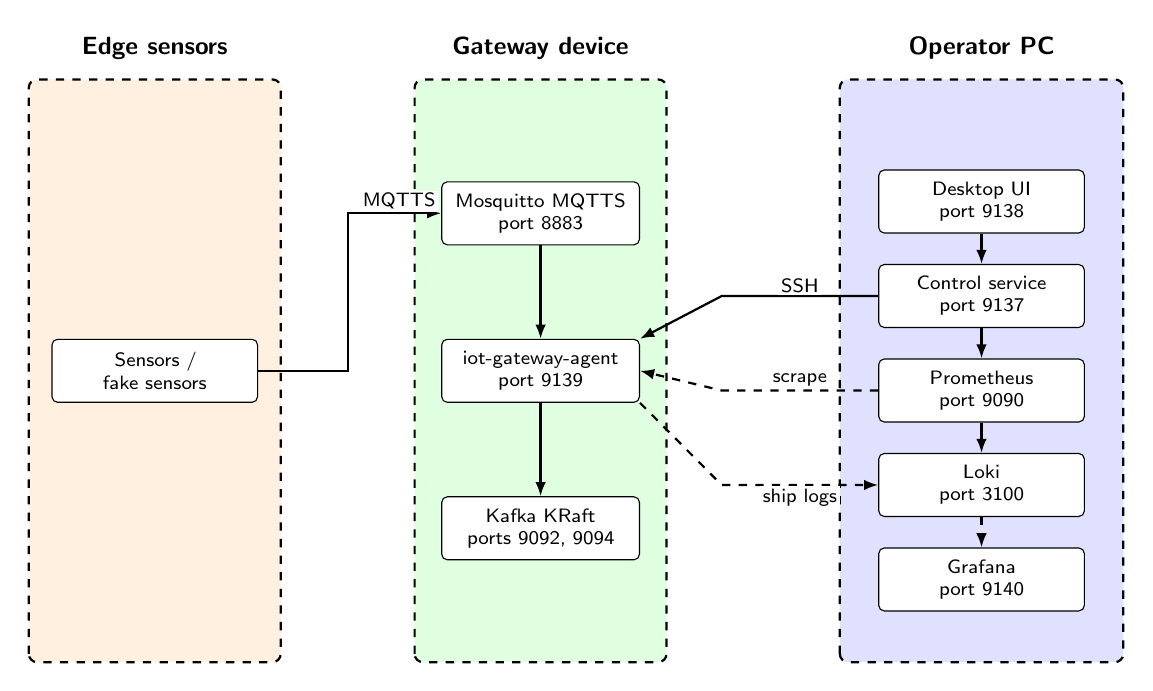
\begin{tikzpicture}[
    every node/.style={font=\scriptsize\sffamily},
    box/.style={
        draw,
        rounded corners=2pt,
        align=center,
        inner sep=3pt,
        minimum height=8mm,
        text width=2.6cm,
        fill=white
    },
    elab/.style={font=\small\sffamily\bfseries},
    lbl/.style={font=\scriptsize\sffamily, fill=white, inner sep=1pt}
]
    % Frames with padding around inner boxes; gaps stay clear
    % Edge: -1.6..1.6   Gateway: 3.3..6.5   PC: 8.7..12.3
    \fill[orange!12, rounded corners=3pt]
        (-1.6,-3.7) rectangle (1.6,3.7);
    \draw[dashed, thick, rounded corners=3pt]
        (-1.6,-3.7) rectangle (1.6,3.7);
    \node[elab] at (0,4.1) {Edge sensors};

    \fill[green!12, rounded corners=3pt]
        (3.3,-3.7) rectangle (6.5,3.7);
    \draw[dashed, thick, rounded corners=3pt]
        (3.3,-3.7) rectangle (6.5,3.7);
    \node[elab] at (4.9,4.1) {Gateway device};

    \fill[blue!12, rounded corners=3pt]
        (8.7,-3.7) rectangle (12.3,3.7);
    \draw[dashed, thick, rounded corners=3pt]
        (8.7,-3.7) rectangle (12.3,3.7);
    \node[elab] at (10.5,4.1) {Operator PC};

    % ---- Edge ----
    \node[box, text width=2.4cm] (sensors) at (0,0)
        {Sensors /\\fake sensors};

    % ---- Gateway (stack), inset from the dashed frame ----
    \node[box, text width=2.3cm] (mqtt)  at (4.9, 2.0)
        {Mosquitto MQTTS\\port 8883};
    \node[box, text width=2.3cm] (agent) at (4.9, 0.0)
        {iot-gateway-agent\\port 9139};
    \node[box, text width=2.3cm] (kafka) at (4.9,-2.0)
        {Kafka KRaft\\ports 9092, 9094};

    % ---- Operator PC (single stack), inset from the frame ----
    \node[box, text width=2.4cm] (ui)   at (10.5, 2.15)
        {Desktop UI\\port 9138};
    \node[box, text width=2.4cm] (cs)   at (10.5, 0.95)
        {Control service\\port 9137};
    \node[box, text width=2.4cm] (prom) at (10.5,-0.25)
        {Prometheus\\port 9090};
    \node[box, text width=2.4cm] (loki) at (10.5,-1.45)
        {Loki\\port 3100};
    \node[box, text width=2.4cm] (graf) at (10.5,-2.65)
        {Grafana\\port 9140};

    % Vertical internals only
    \draw[archflow] (mqtt) -- (agent);
    \draw[archflow] (agent) -- (kafka);
    \draw[archflow] (ui) -- (cs);
    \draw[archflow] (cs) -- (prom);
    \draw[archflow] (prom) -- (loki);
    \draw[archflowsoft] (loki) -- (graf);

    % Interface points sit in the gap (not on the Gateway border)
    \coordinate (gSSH) at (7.2, 0.95);
    \coordinate (gSCR) at (7.2,-0.25);
    \coordinate (gSHP) at (7.2,-1.45);

    % ---- Cross-links: horizontals only in the gaps ----
    \draw[archflow]
        (sensors.east) -- (2.45,0) -- (2.45,2.0) --
        node[lbl, above, pos=0.55] {MQTTS} (mqtt.west);

    \draw[archflow]
        (cs.west) -- node[lbl, above] {SSH} (gSSH)
        -- (agent.north east);
    \draw[archflowsoft]
        (prom.west) -- node[lbl, above] {scrape} (gSCR)
        -- (agent.east);
    \draw[archflowsoft]
        (agent.south east) -- (gSHP)
        -- node[lbl, below] {ship logs} (loki.west);
\end{tikzpicture}%
}
\caption{Top-level architecture of IoT-SecureGate.}
\label{fig:arch-toplevel}
\end{figure}

The split matches the operational context of
Chapter~\ref{ch:requirements}: one product, two runtimes,
with the gateway as the controlled entry point for inbound
plant telemetry.

\section{Monitoring Application Overview}
\label{sec:arch-monitoring-overview}

Figure~\ref{fig:arch-monitoring} summarises the operator
runtime as two regions on the PC. The desktop package
holds the Wizard/UI, control service, local registry,
OS keyring, and the FakeCertRenewer used for laboratory
fakes. Beside it, a local observability stack runs Loki,
Prometheus, and Grafana as native processes under the
application data directory so routine use does not depend
on Docker (FR-13, NFR-1, NFR-2). The control service
queries Loki and Prometheus; the UI opens Grafana in the
system browser. Sensitive material for CA signing and
day-2 privilege lives in the OS keyring (FR-14, NFR-6).

\begin{figure}[htbp]
\centering
\resizebox{\textwidth}{!}{%
\begin{tikzpicture}[
    every node/.style={font=\scriptsize\sffamily},
    box/.style={
        draw,
        rounded corners=2pt,
        align=center,
        inner sep=3pt,
        minimum height=8mm,
        text width=2.4cm,
        fill=white
    },
    elab/.style={font=\small\sffamily\bfseries},
    lbl/.style={font=\scriptsize\sffamily, fill=white, inner sep=1pt}
]
    % architecture.md §2: desktop package | local observability
    \fill[blue!10, rounded corners=3pt]
        (-0.3,-3.9) rectangle (6.8,3.6);
    \draw[dashed, thick, rounded corners=3pt]
        (-0.3,-3.9) rectangle (6.8,3.6);
    \node[elab] at (3.25,4.0)
        {IoT Gateway Monitor};

    \fill[cyan!10, rounded corners=3pt]
        (8.8,-3.9) rectangle (12.6,3.6);
    \draw[dashed, thick, rounded corners=3pt]
        (8.8,-3.9) rectangle (12.6,3.6);
    \node[elab] at (10.7,4.0) {Local observability};

    % ---- Desktop package (two columns, padded) ----
    \node[box] (wiz)   at (1.4, 2.1) {Wizard / UI\\port 9138};
    \node[box] (ctrl)  at (4.7, 2.1) {Control service\\port 9137};
    \node[box] (reg)   at (1.4, 0.0) {registry.sqlite\\gateways + devices};
    \node[box] (key)   at (4.7, 0.0) {OS keyring\\CA · sudo · PIN};
    \node[box] (renew) at (4.7,-2.1) {FakeCertRenewer\\(fakes only)};

    % ---- Local observability (aligned with cross-link lanes) ----
    \node[box] (loki) at (10.7, 2.1) {Loki\\port 3100};
    \node[box] (prom) at (10.7, 0.0) {Prometheus\\port 9090};
    \node[box] (graf) at (10.7,-2.1) {Grafana HTTPS\\port 9140};

    % ---- Intra-desktop ----
    \draw[archflow] (wiz) -- (ctrl);
    \draw[archflow] (wiz) -- (reg);
    \draw[archflow] (ctrl) -- (key);
    \draw[archflow] (key) -- (renew);
    \draw[archflow] (reg.east) -- (key.west);

    % Gap waypoints (clear of both frame borders)
    \coordinate (gLoki) at (7.8, 2.1);
    \coordinate (gProm) at (7.8, 0.0);
    \coordinate (gGraf) at (7.8,-2.1);

    % Control → Loki / Prometheus (query APIs)
    \draw[archflow]
        (ctrl.east) -- node[lbl, above] {query} (gLoki)
        -- (loki.west);
    \draw[archflow]
        (key.east) -- node[lbl, above] {query} (gProm)
        -- (prom.west);

    % Wizard / UI → Grafana (system browser): mid-aisle down,
    % under FakeCertRenewer, label only in the inter-frame gap
    \draw[archflowsoft]
        (wiz.east) -- (3.05,2.1) -- (3.05,-3.35) --
        node[lbl, below, pos=0.72] {open browser}
        (7.8,-3.35) -- (gGraf) -- (graf.west);

    % Grafana reads the local stack
    \draw[archflowsoft] (graf) -- (prom);
    \draw[archflowsoft] (prom) -- (loki);
\end{tikzpicture}%
}
\caption{Overview of the monitoring application on the
operator PC.}
\label{fig:arch-monitoring}
\end{figure}

Chapter~\ref{ch:monitoring} details how this runtime is
prepared, how it installs gateways and onboards devices,
and how its operational workflows use the local stack.

\section{Gateway Overview}
\label{sec:arch-gateway-overview}

Figure~\ref{fig:arch-gateway} summarises the edge
runtime from \texttt{architecture.md}. Real sensors and
laboratory fakes share one MQTTS ingress into Mosquitto
(fakes reach the broker through the on-gateway
\texttt{iotgw-fake} bridge). The decrypt worker opens
accepted envelopes, writes \texttt{sensor\_data.log}, and
produces Kafka topics. The Loki shipper pushes log lines
to the operator PC; Prometheus scrapes agent metrics on
port~9139.

\begin{figure}[htbp]
\centering
\resizebox{\textwidth}{!}{%
\begin{tikzpicture}[
    every node/.style={font=\scriptsize\sffamily},
    box/.style={
        draw,
        rounded corners=2pt,
        align=center,
        inner sep=4pt,
        minimum height=10mm,
        text width=2.8cm,
        fill=white
    },
    elab/.style={font=\small\sffamily\bfseries},
    lbl/.style={font=\scriptsize\sffamily, fill=white, inner sep=1pt}
]
    % Edge: -1.8..1.8   Gateway: 3.2..9.8   Operator: 11.0..14.6
    \fill[orange!12, rounded corners=3pt]
        (-1.8,-3.5) rectangle (1.8,3.5);
    \draw[dashed, thick, rounded corners=3pt]
        (-1.8,-3.5) rectangle (1.8,3.5);
    \node[elab] at (0,3.9) {Edge publishers};

    \fill[green!12, rounded corners=3pt]
        (3.2,-3.9) rectangle (9.8,3.5);
    \draw[dashed, thick, rounded corners=3pt]
        (3.2,-3.9) rectangle (9.8,3.5);
    \node[elab] at (6.5,3.9) {Gateway device};

    \fill[blue!12, rounded corners=3pt]
        (11.0,-3.9) rectangle (14.6,3.5);
    \draw[dashed, thick, rounded corners=3pt]
        (11.0,-3.9) rectangle (14.6,3.5);
    \node[elab] at (12.8,3.9) {Operator PC};

    % ---- Edge publishers ----
    \node[box] (real) at (0,1.4) {Real sensors};
    \node[box] (labs) at (0,-1.2) {Lab fakes};

    % ---- Gateway: one vertical pipeline + side outputs ----
    \node[box, text width=3.2cm] (mosq) at (6.5, 2.2)
        {Mosquitto MQTTS\\port 8883 (mTLS)};
    \node[box, text width=3.2cm] (dec) at (6.5, 0.55)
        {Decrypt worker};
    \node[box] (log) at (5.0,-1.0)
        {sensor\_data.log};
    \node[box] (kafka) at (8.0,-1.0)
        {Kafka KRaft\\ports 9092, 9094};
    \node[box] (ship) at (5.0,-2.5)
        {Loki shipper};
    \node[box] (met) at (8.0,-2.5)
        {HTTP, port 9139\\/metrics · /health};

    % ---- Operator ----
    \node[box] (oloki) at (12.8, 1.0) {Operator Loki\\port 3100};
    \node[box] (oprom) at (12.8,-2.5) {Operator Prometheus\\port 9090};

    % ---- Shared MQTTS merge in the gap (paths overlap) ----
    % Feeders have no arrow tips so nothing stops mid-gap;
    % only the shared stem into Mosquitto is arrowed.
    \coordinate (merge) at (2.5, 2.2);
    \draw[thick] (real.east) -- (2.5,1.4) -- (merge);
    \draw[thick] (labs.east) -- (2.5,-1.2) -- (merge);
    \draw[archflow]
        (merge) -- node[lbl, above] {MQTTS} (mosq.west);

    % ---- Intra-gateway pipeline ----
    \draw[archflow] (mosq) -- (dec);
    \draw[archflow] (dec.south) -- (6.5,-0.3) -- (5.0,-0.3)
        -- (log.north);
    \draw[archflow] (dec.south) -- (6.5,-0.3) -- (8.0,-0.3)
        -- (kafka.north);
    \draw[archflow] (log) -- (ship);

    % ---- Operator links ----
    \draw[archflowsoft]
        (oprom.west) --
        node[lbl, above] {scrape} (met.east);
    % ship stays below scrape, then climbs outside Operator PC
    \draw[archflowsoft]
        (ship.south) -- (5.0,-3.45) -- (14.95,-3.45) -- (14.95,1.0)
        -- node[lbl, right, pos=0.4] {ship logs} (oloki.east);
\end{tikzpicture}%
}
\caption{Overview of the gateway runtime and its links to
operator observability.}
\label{fig:arch-gateway}
\end{figure}

Operational health views use the canonical application
order Agent $\rightarrow$ MQTT $\rightarrow$ Decrypt
$\rightarrow$ Shipper $\rightarrow$ Kafka.
Chapter~\ref{ch:gateway} expands how the agent and
broker handle inbound traffic;
Chapter~\ref{ch:encryption} expands how envelopes are
opened and validated.

\section{Control Plane and Data Plane}
\label{sec:arch-planes}

IoT-SecureGate separates \emph{control} actions from
\emph{data} movement, as shown in
Figure~\ref{fig:arch-planes}.

\begin{itemize}
    \item \textbf{Control plane.}
    The monitoring application reaches the gateway over
    SSH to provision the agent stack and to apply day-2
    changes such as device registration, ACL updates,
    certificate work, and Auto prevent policy. Registry
    state and operator secrets stay on the PC.
    \item \textbf{Data plane.}
    Sensors publish on MQTTS into Mosquitto. After decrypt
    and schema validation, accepted plaintext is stored
    locally and in Kafka. Metrics are scraped over HTTP
    from the agent; logs are pushed to operator Loki.
    Grafana reads that local stack and the gateway's Kafka
    EXTERNAL listener.
\end{itemize}

\begin{figure}[htbp]
\centering
\resizebox{\textwidth}{!}{%
\begin{tikzpicture}[
    every node/.style={font=\scriptsize\sffamily},
    box/.style={
        draw,
        rounded corners=2pt,
        align=center,
        inner sep=3pt,
        minimum height=8mm,
        text width=2.6cm,
        fill=white
    },
    elab/.style={font=\small\sffamily\bfseries},
    lbl/.style={font=\scriptsize\sffamily, align=center,
        fill=white, inner sep=1pt},
    lane/.style={font=\small\sffamily\bfseries, rotate=90}
]
    % architecture.md §1: columns are hosts, rows are planes
    % Gutter -2.35 · Edge -1.7..1.5 · Gateway 3.5..8.6 · PC 10.8..15.0
    % Control band 2.0..3.7 · data rows 1.05, -0.1, -1.25, -2.4, -3.55
    \node[elab] at (-0.1,4.05) {Edge sensors};
    \node[elab] at (6.05,4.05) {Gateway device};
    \node[elab] at (12.9,4.05) {Operator PC};
    \node[lane] at (-2.35,2.85) {Control plane};
    \node[lane] at (-2.35,-1.3) {Data plane};

    % ---- Control band: SSH reaches the gateway and stops there,
    % so the sensor column carries no frame in this row ----
    \fill[green!12, rounded corners=3pt]
        (3.5,2.0) rectangle (8.6,3.7);
    \draw[dashed, thick, rounded corners=3pt]
        (3.5,2.0) rectangle (8.6,3.7);
    \fill[blue!12, rounded corners=3pt]
        (10.8,2.0) rectangle (15.0,3.7);
    \draw[dashed, thick, rounded corners=3pt]
        (10.8,2.0) rectangle (15.0,3.7);

    \node[box, text width=3.0cm] (sshd) at (6.05,2.85)
        {SSH daemon, port 22\\registration · ACL\\certs · Auto prevent};
    \node[box, text width=3.2cm] (cs) at (12.9,2.85)
        {Control service\\port 9137 · playbooks};

    \draw[archflow] (cs.west) -- node[lbl, above] {SSH} (sshd.east);

    % ---- Data band: one gateway endpoint per cross-link lane,
    % each frame sized to the rows it actually holds ----
    \fill[orange!12, rounded corners=3pt]
        (-1.7,0.45) rectangle (1.5,1.6);
    \draw[dashed, thick, rounded corners=3pt]
        (-1.7,0.45) rectangle (1.5,1.6);
    \fill[green!12, rounded corners=3pt]
        (3.5,-4.15) rectangle (8.6,1.6);
    \draw[dashed, thick, rounded corners=3pt]
        (3.5,-4.15) rectangle (8.6,1.6);
    \fill[blue!12, rounded corners=3pt]
        (10.8,-4.15) rectangle (15.0,-0.7);
    \draw[dashed, thick, rounded corners=3pt]
        (10.8,-4.15) rectangle (15.0,-0.7);

    \node[box] (sensors) at (-0.1,1.05) {Sensors /\\fake sensors};
    \node[box, text width=3.2cm] (mosq) at (6.05,1.05)
        {Mosquitto MQTTS\\port 8883 · mTLS};
    \node[box, text width=3.2cm] (dec) at (6.05,-0.1)
        {Decrypt worker\\sensor\_data.log};
    \node[box, text width=3.2cm] (kafka) at (6.05,-1.25)
        {Kafka KRaft\\ports 9092, 9094};
    \node[box, text width=3.2cm] (met) at (6.05,-2.4)
        {Agent HTTP, port 9139\\/metrics · /v1/health};
    \node[box, text width=3.2cm] (ship) at (6.05,-3.55)
        {Loki shipper};

    % Operator side, aligned with the gateway rows its lanes belong to
    \node[box, text width=3.2cm] (graf) at (12.9,-1.25)
        {Grafana HTTPS\\port 9140};
    \node[box, text width=3.2cm] (prom) at (12.9,-2.4)
        {Prometheus\\port 9090};
    \node[box, text width=3.2cm] (loki) at (12.9,-3.55)
        {Loki\\port 3100};

    % Inbound path; gateway internals beyond ingress are Figures 4.1/4.3
    \draw[archflow]
        (sensors.east) -- node[lbl, above] {MQTTS} (mosq.west);
    \draw[archflow] (mosq) -- (dec);

    % Observability lanes, straight across the gap
    \draw[archflowsoft]
        (graf.west) -- node[lbl, above] {datasource} (kafka.east);
    \draw[archflowsoft]
        (prom.west) -- node[lbl, above] {scrape} (met.east);
    \draw[archflowsoft]
        (ship.east) -- node[lbl, above] {ship logs} (loki.west);

    % Grafana reads the local stack
    \draw[archflowsoft] (graf) -- (prom);
    \draw[archflowsoft] (prom) -- (loki);
\end{tikzpicture}%
}
\caption{The control and data planes across the three
hosts.}
\label{fig:arch-planes}
\end{figure}

That separation keeps privileged configuration off the
sensor path and keeps high-volume telemetry off the SSH
session used for administration.

\section{End-to-End Inbound Path}
\label{sec:arch-datapath}

Figure~\ref{fig:arch-datapath} is the inbound path that
FR-1 through FR-4 require. Its decisive property is the
order in which those requirements are met, because admission
is settled before any payload is examined. The broker applies
the credential and topic checks that registration installed,
and the agent is itself a client of that broker, so a message
reaches the decrypt stage only once the broker has accepted
it (FR-2). Publication is possible only where registration
has bound a device identity to its MQTT credential, its topic
permissions, a client certificate under the gateway CA, and a
reserved storage topic (FR-1).

Opening a message is then compulsory rather than optional:
the gateway decrypts what it accepts, because the plaintext
it stores must be the plaintext it examined. A payload that
cannot be opened, or that does not match the schema
registered for its device, is refused before anything is
recorded (FR-3); the shape check belongs to the envelope
path, so a legacy wrapper is honoured only while envelope
enforcement is disabled, and then on its wrapper key alone.
Accepted output divides into the two sinks FR-4 names: a
local sensor data log whose lines are forwarded to the
operator, and one topic per registered device.

\begin{figure}[htbp]
\centering
\resizebox{\textwidth}{!}{%
\begin{tikzpicture}[
    every node/.style={font=\scriptsize\sffamily},
    box/.style={
        draw,
        rounded corners=2pt,
        align=center,
        inner sep=3pt,
        minimum height=8mm,
        text width=2.6cm,
        fill=white
    },
    elab/.style={font=\small\sffamily\bfseries},
    lbl/.style={font=\scriptsize\sffamily, align=center,
        fill=white, inner sep=1pt}
]
    % architecture.md §4 + decrypt_worker.py: the accepted path runs down the
    % gateway column; gate failures leave it onto the deny rail
    % Columns: Edge -1.9..1.7 · Gateway 3.5..8.7 · PC 10.8..15.0
    % Rows: 2.6, 1.3, 0.0, -1.3, -2.6 · deny row -3.9 · reject rail x=8.45
    \node[elab] at (-0.1,3.75) {Edge sensors};
    \node[elab] at (6.05,3.75) {Gateway device};
    \node[elab] at (12.9,3.75) {Operator PC};

    \fill[orange!12, rounded corners=3pt]
        (-1.9,1.75) rectangle (1.7,3.35);
    \draw[dashed, thick, rounded corners=3pt]
        (-1.9,1.75) rectangle (1.7,3.35);
    \fill[green!12, rounded corners=3pt]
        (3.5,-4.75) rectangle (8.7,3.35);
    \draw[dashed, thick, rounded corners=3pt]
        (3.5,-4.75) rectangle (8.7,3.35);
    \fill[blue!12, rounded corners=3pt]
        (10.8,-3.3) rectangle (15.0,-1.9);
    \draw[dashed, thick, rounded corners=3pt]
        (10.8,-3.3) rectangle (15.0,-1.9);

    \node[box, text width=3.0cm] (sensors) at (-0.1,2.6)
        {1.\ Sensor / fake sensor\\publish\\env/key + env/data};
    \node[box, text width=3.6cm] (mosq) at (6.05,2.6)
        {2.\ Mosquitto MQTTS\\port 8883 · password\\· mTLS · topic ACL};
    \node[box, text width=3.6cm] (sub) at (6.05,1.3)
        {3.\ Agent subscribe sensors/\#\\TLS over localhost};
    \node[box, text width=3.6cm] (open) at (6.05,0.0)
        {4.\ Pair by msg\_id · unwrap CEK\\AES-128-GCM · schema\\legacy Fernet where allowed};
    \node[box, text width=3.6cm] (sinks) at (6.05,-1.3)
        {5.\ sensor\_data.log · Kafka\\sensor.\textless device\_id\textgreater{}};
    \node[box, text width=3.6cm] (ship) at (6.05,-2.6)
        {6.\ Loki shipper\\tail + POST batches};
    \node[box, text width=3.6cm] (deny) at (6.05,-3.9)
        {Denied / invalid records\\ACL · handshake · replay\\unwrap · schema · timeout};
    \node[box, text width=3.2cm] (loki) at (12.9,-2.6)
        {Operator Loki\\port 3100};

    % ---- Accepted path ----
    \draw[archflow]
        (sensors.east) -- node[lbl, above] {MQTTS} (mosq.west);
    \draw[archflow] (mosq) -- (sub);
    \draw[archflow] (sub) -- (open);
    \draw[archflow] (open) -- (sinks);
    \draw[archflow] (sinks) -- (ship);
    \draw[archflowsoft]
        (ship.east) -- node[lbl, above] {HTTP push} (loki.west);

    % ---- Gate failures leave the path (feeders plain, stem arrowed) ----
    \coordinate (rej) at (8.45,-3.9);
    \draw[thick, black!55, dashed]
        (mosq.east) -- (8.45,2.6) -- (rej);
    \draw[thick, black!55, dashed]
        (open.east) -- (8.45,0.0) -- (rej);
    \draw[archflowsoft] (rej) -- (deny.east);
\end{tikzpicture}%
}
\caption{The stages a published message passes on the
inbound path.}
\label{fig:arch-datapath}
\end{figure}

Failed authentication, authorization, decrypt, or schema
checks do not enter the accepted storage path; they feed
deny and invalid signalling used for operator visibility
and response (FR-9--FR-11). Chapter~\ref{ch:gateway}
describes this path as gateway behaviour;
Chapter~\ref{ch:encryption} describes the envelope open
in detail.

\section{Layered Message Protection Overview}
\label{sec:arch-protection}

Figure~\ref{fig:arch-protection} places each layer at the
position on the path where its material actually rests;
Table~\ref{tab:arch-protection-layers} states what each
layer as a whole answers.

Independence is the point. The broker sees two opaque
halves, so a connection it accepts proves only that its
holder may publish, and halves that arrive apart cannot be
authenticated until both are present, because the stamp
binding them is computed from material each half carries.

\begin{figure}[htbp]
\centering
\resizebox{\textwidth}{!}{%
\begin{tikzpicture}[
    every node/.style={font=\scriptsize\sffamily},
    box/.style={
        draw,
        rounded corners=2pt,
        align=center,
        inner sep=3pt,
        minimum height=8mm,
        text width=2.6cm,
        fill=white
    },
    elab/.style={font=\small\sffamily\bfseries},
    lane/.style={
        font=\small\sffamily\bfseries,
        align=right,
        text width=2.0cm
    }
]
    % envelope_v1.py seal/open + decrypt_worker.py gates + broker.py listener:
    % rows are layers, columns are where a layer's material actually rests
    % Row names right-aligned at -2.9 · Edge -1.7..2.3 · Wire 3.8..7.8
    % Gateway 9.3..13.8 · Rows 2.6, 1.3, 0.0, -1.3, -2.6 · frames -3.3..3.3
    \node[elab] at (0.3,3.75) {Edge sensors};
    \node[elab] at (5.8,3.75) {On the wire};
    \node[elab] at (11.55,3.75) {Gateway device};

    \node[lane] at (-2.9,2.6) {Transport};
    \node[lane] at (-2.9,1.3) {Binding};
    \node[lane] at (-2.9,0.0) {Key wrap};
    \node[lane] at (-2.9,-1.3) {Payload};
    \node[lane] at (-2.9,-2.6) {Shape};

    \fill[orange!12, rounded corners=3pt]
        (-1.7,-3.3) rectangle (2.3,3.3);
    \draw[dashed, thick, rounded corners=3pt]
        (-1.7,-3.3) rectangle (2.3,3.3);
    \fill[gray!10, rounded corners=3pt]
        (3.8,-3.3) rectangle (7.8,3.3);
    \draw[dashed, thick, rounded corners=3pt]
        (3.8,-3.3) rectangle (7.8,3.3);
    \fill[green!12, rounded corners=3pt]
        (9.3,-3.3) rectangle (13.8,3.3);
    \draw[dashed, thick, rounded corners=3pt]
        (9.3,-3.3) rectangle (13.8,3.3);

    \node[box, text width=3.5cm] at (0.3,2.6)
        {MQTT credential +\\client certificate};
    \node[box, text width=3.5cm] at (5.8,2.6)
        {MQTTS, port 8883\\TLS session};
    \node[box, text width=3.9cm] at (11.55,2.6)
        {credential\\certificate · topic ACL};

    \node[box, text width=3.5cm] at (0.3,1.3)
        {binding key from\\registration};
    \node[box, text width=3.5cm] at (5.8,1.3)
        {one stamp, equal\\in both halves};
    \node[box, text width=3.9cm] at (11.55,1.3)
        {recomputed only\\from both halves};

    \node[box, text width=3.5cm] at (0.3,0.0)
        {pre-shared secret or\\the day certificate};
    \node[box, text width=3.5cm] at (5.8,0.0)
        {wrapped key\\on its own topic};
    \node[box, text width=3.9cm] at (11.55,0.0)
        {unwraps within\\one day of today};

    \node[box, text width=3.5cm] at (0.3,-1.3)
        {fresh content key\\per message};
    \node[box, text width=3.5cm] at (5.8,-1.3)
        {ciphertext\\second topic};
    \node[box, text width=3.9cm] at (11.55,-1.3)
        {AES-128-GCM open\\with the ids as AAD};

    \node[box, text width=3.5cm] at (0.3,-2.6)
        {declares which shape\\it claims};
    \node[box, text width=3.5cm] at (5.8,-2.6)
        {the id, bound into\\stamp and ciphertext};
    \node[box, text width=3.9cm] at (11.55,-2.6)
        {holds the shape;\\checks plaintext};
\end{tikzpicture}%
}
\caption{Where the material behind each protection layer
rests.}
\label{fig:arch-protection}
\end{figure}

\begin{table}[H]
\centering
{\small
\begin{tabularx}{\textwidth}{@{}p{2.4cm}Y Y@{}}
\toprule
\textbf{Layer} & \textbf{Mechanism} & \textbf{Answers} \\
\midrule
Transport
& MQTTS with mutual TLS, Mosquitto password, and topic ACL
& Who may connect and publish \\
\midrule
Application
& Envelope v1 (\texttt{v1-psk} / \texttt{v1-ecdhe})
& Confidentiality after TLS termination \\
\midrule
Schema
& Registered JSON schema on the gateway
& Message shape after decrypt \\
\midrule
Day material
& Daily Message Encryption Certificate (DMEC)
& Day-scoped wrap for \texttt{v1-ecdhe} \\
\bottomrule
\end{tabularx}}
\caption{Protection layers on the gateway inbound path
(overview).}
\label{tab:arch-protection-layers}
\end{table}

Profiles, topic pairing, replay resistance, and the full
encrypt/decrypt workflow are specified in
Chapter~\ref{ch:encryption}. Legacy Fernet remains
accepted only where still configured; the architectural
target is envelope v1 on MQTTS.

\section{Deployment Topology and Ports}
\label{sec:arch-ports}

Tables~\ref{tab:arch-ports-pc} and
Table~\ref{tab:arch-ports-gw} list the default listening
port of every component on a trusted plant or laboratory
LAN (NFR-9). A port list cannot show direction, so
Figure~\ref{fig:arch-topology} draws which side opens each
connection across that LAN, on the same three hosts as
Figure~\ref{fig:arch-toplevel}. Direction is what decides
which components must accept connections from a machine
that is not their own.

\begin{table}[H]
\centering
{\small
\begin{tabularx}{\textwidth}{@{}p{2.8cm}p{4.2cm}Y@{}}
\toprule
\textbf{Component} & \textbf{Listening on} & \textbf{Role} \\
\midrule
Control service & localhost, port 9137 & Registry, playbooks, queries \\
Wizard / UI & localhost, port 9138 & Desktop interface and API proxy \\
Loki & all interfaces, port 3100 & Log target for the gateway shipper \\
Prometheus & all interfaces, port 9090 & Scrapes gateway agent metrics \\
Grafana & localhost, port 9140 (HTTPS) & Local dashboards in system browser \\
\bottomrule
\end{tabularx}}
\caption{Operator PC ports for the monitoring application.}
\label{tab:arch-ports-pc}
\end{table}

\begin{table}[H]
\centering
{\small
\begin{tabularx}{\textwidth}{@{}p{2.8cm}p{4.2cm}Y@{}}
\toprule
\textbf{Component} & \textbf{Listening on} & \textbf{Role} \\
\midrule
Agent HTTP & all interfaces, port 9139 & Metrics, health, day-key helpers \\
Mosquitto MQTTS & all interfaces, port 8883 & Sensor ingress (password + client cert) \\
Kafka INTERNAL & localhost, port 9092 & Agent produce path \\
Kafka EXTERNAL & gateway address, port 9094 & Trusted-LAN Grafana datasource \\
\bottomrule
\end{tabularx}}
\caption{Gateway device ports.}
\label{tab:arch-ports-gw}
\end{table}

\begin{figure}[htbp]
\centering
\resizebox{\textwidth}{!}{%
\begin{tikzpicture}[
    every node/.style={font=\scriptsize\sffamily},
    box/.style={
        draw,
        rounded corners=2pt,
        align=center,
        inner sep=3pt,
        minimum height=8mm,
        text width=2.6cm,
        fill=white
    },
    elab/.style={font=\small\sffamily\bfseries},
    lbl/.style={font=\scriptsize\sffamily, align=center,
        fill=white, inner sep=1pt}
]
    % prometheus.yml scrape target + provisioned datasources + the single
    % firewall rule: each column lists a host's own listeners, and every
    % arrow runs from the component that opens the connection to the socket
    % Columns: Edge -1.9..1.7 · Gateway 3.5..8.7 · PC 10.8..15.0
    % Rows 2.5, 1.25, 0.0, -1.25, -2.5 · host frames 3.0/-3.0 · Edge 0.75..1.75
    \node[elab] at (-0.1,3.4) {Edge sensors};
    \node[elab] at (6.1,3.4) {Gateway device};
    \node[elab] at (12.9,3.4) {Operator PC};

    \fill[green!12, rounded corners=3pt]
        (3.5,-3.0) rectangle (8.7,3.0);
    \draw[dashed, thick, rounded corners=3pt]
        (3.5,-3.0) rectangle (8.7,3.0);
    \fill[blue!12, rounded corners=3pt]
        (10.8,-3.0) rectangle (15.0,3.0);
    \draw[dashed, thick, rounded corners=3pt]
        (10.8,-3.0) rectangle (15.0,3.0);
    \fill[orange!12, rounded corners=3pt]
        (-1.9,0.75) rectangle (1.7,1.75);
    \draw[dashed, thick, rounded corners=3pt]
        (-1.9,0.75) rectangle (1.7,1.75);

    \node[box, text width=4.4cm] (sshd) at (6.1,2.5)
        {SSH daemon, port 22\\registration · day-2};
    \node[box, text width=3.5cm] (shell) at (12.9,2.5)
        {Desktop shell\\+ control service};

    \node[box, text width=3.0cm] (sensors) at (-0.1,1.25)
        {Sensors\\real · fake};
    \node[box, text width=4.4cm] (mosq) at (6.1,1.25)
        {Mosquitto MQTTS, port 8883};
    \node[box, text width=3.5cm] (loop) at (12.9,1.25)
        {localhost only:\\UI · Control · Grafana};

    \node[box, text width=4.4cm] (agent) at (6.1,0.0)
        {Agent HTTP, port 9139};
    \node[box, text width=3.5cm] (prom) at (12.9,0.0)
        {Prometheus, port 9090};

    \node[box, text width=4.4cm] (kafka) at (6.1,-1.25)
        {Kafka EXTERNAL, port 9094};
    \node[box, text width=3.5cm] (graf) at (12.9,-1.25)
        {Grafana\\Kafka datasources};

    \node[box, text width=4.4cm] (ship) at (6.1,-2.5)
        {Loki shipper};
    \node[box, text width=3.5cm] (loki) at (12.9,-2.5)
        {Loki, port 3100};

    \draw[archflow]
        (shell.west) -- node[lbl, above] {SSH} (sshd.east);
    \draw[archflow]
        (sensors.east) -- node[lbl, above] {publish} (mosq.west);
    \draw[archflow]
        (prom.west) -- node[lbl, above] {scrape} (agent.east);
    \draw[archflow]
        (graf.west) -- node[lbl, above] {query} (kafka.east);
    \draw[archflow]
        (ship.east) -- node[lbl, above] {ship} (loki.west);
\end{tikzpicture}%
}
\caption{Which side opens each connection across the plant
LAN.}
\label{fig:arch-topology}
\end{figure}

\section{Trust Material and Secrets}
\label{sec:arch-secrets}

Figure~\ref{fig:arch-secrets} shows which machine holds
which part of the trust material, and what is allowed to
move between them. Two splits carry the design.
The gateway owns a certificate authority: its private
key, its certificate, and the counter that keeps the
serial numbers it issues unique. It does not hold the
passphrase that unlocks that key, which stays on the
operator PC and reaches the gateway only for the
duration of one signing. The other split runs the
opposite way. Every device key pair is minted on the
operator PC, so the machine that signs a device's
request is never the machine that also sees the private
key behind it. What the gateway does receive is the
material for opening a device's messages: one set of
envelope keys per registered device, which the device
also holds in order to seal them.

The remaining secrets stay on the operator PC---each
gateway's SSH credential and sudo password, the
passphrase for that gateway's authority, and a hash of
the local administrator PIN---held in the OS keyring,
where a permission-restricted file under the
application's own directory stands in if the operating
system offers no keyring backend. A local proxy reads
them from there on the operator's behalf, so a routine
maintenance action does not ask for the same secret
twice (FR-14). Where privileged work must run on the
gateway, the password is written to the standard input
of the command that consumes it, and the authority
passphrase to a short-lived file readable only by its
owner; neither is placed on a remote command line, where
the process list would expose it (NFR-6).

\begin{figure}[htbp]
\centering
\resizebox{\textwidth}{!}{%
\begin{tikzpicture}[
    every node/.style={font=\scriptsize\sffamily},
    box/.style={
        draw,
        rounded corners=2pt,
        align=center,
        inner sep=3pt,
        minimum height=8mm,
        text width=2.6cm,
        fill=white
    },
    elab/.style={font=\small\sffamily\bfseries},
    lbl/.style={font=\scriptsize\sffamily, align=center,
        fill=white, inner sep=1pt}
]
    % each arrow is one crossing of material, and the two absent ones carry
    % the argument: the CA private key never leaves the gateway, and no
    % device key pair ever reaches it
    % Device -2.4..0.8 · Gateway 1.4..6.6 · PC 9.6..13.8
    % Rows 1.55, 0.0, -1.55 · host frames 2.5/-2.5 · delivery rail -3.5
    \node[elab] at (4.0,2.9) {Gateway device};
    \node[elab] at (11.7,2.9) {Operator PC};

    \fill[green!12, rounded corners=3pt]
        (1.4,-2.5) rectangle (6.6,2.5);
    \draw[dashed, thick, rounded corners=3pt]
        (1.4,-2.5) rectangle (6.6,2.5);
    \fill[blue!12, rounded corners=3pt]
        (9.6,-2.5) rectangle (13.8,2.5);
    \draw[dashed, thick, rounded corners=3pt]
        (9.6,-2.5) rectangle (13.8,2.5);

    \node[box, text width=4.4cm] (ca) at (4.0,1.55)
        {Certificate authority\\private key stays here\\unlocked only to sign};
    \node[box, text width=4.4cm] (brk) at (4.0,0.0)
        {Broker identity\\server certificate · ACL\\· client password file};
    \node[box, text width=4.4cm] (env) at (4.0,-1.55)
        {Envelope key material\\one file per device};

    \node[box, text width=3.5cm] (key) at (11.7,1.55)
        {OS keyring\\SSH · sudo · CA\\passphrase · PIN};
    \node[box, text width=3.5cm] (reg) at (11.7,0.0)
        {Operator registry\\gateways · devices};
    \node[box, text width=3.5cm] (mint) at (11.7,-1.55)
        {Mints device key pairs\\and signing requests};

    \node[box, text width=3.0cm] (dev) at (-0.8,0.0)
        {Sensor device\\its key pair and\\its envelope keys};

    \draw[archflow]
        (key.west) -- node[lbl, above] {passphrase and\\sudo password} (ca.east);
    \draw[archflow]
        (mint.west) -- node[lbl, above] {envelope keys,\\not the key pair} (env.east);
    \draw[archflow]
        (mint.south) -- (11.7,-3.5)
        -- node[lbl, above] {delivered to the device} (-0.8,-3.5)
        -- (dev.south);
\end{tikzpicture}%
}
\caption{Which machine holds each half of the trust material.}
\label{fig:arch-secrets}
\end{figure}

Ordinary settings files and application logs are not the
store for those secrets. Certificate lifecycle and
related workflows are detailed with the runtimes that
implement them.

\section{Delivery of the Software}
\label{sec:arch-delivery}

What is built automatically in this platform is built by one
pipeline. Figure~\ref{fig:arch-delivery} draws it, and this section
fixes what starts a build, what kind of machine runs it, what comes
out of it, and where that is published. What an operator's machine
does with the file afterwards, and what the edge host is given, is
told with the two runtimes themselves.

\begin{figure}[htbp]
\centering
\resizebox{\textwidth}{!}{%
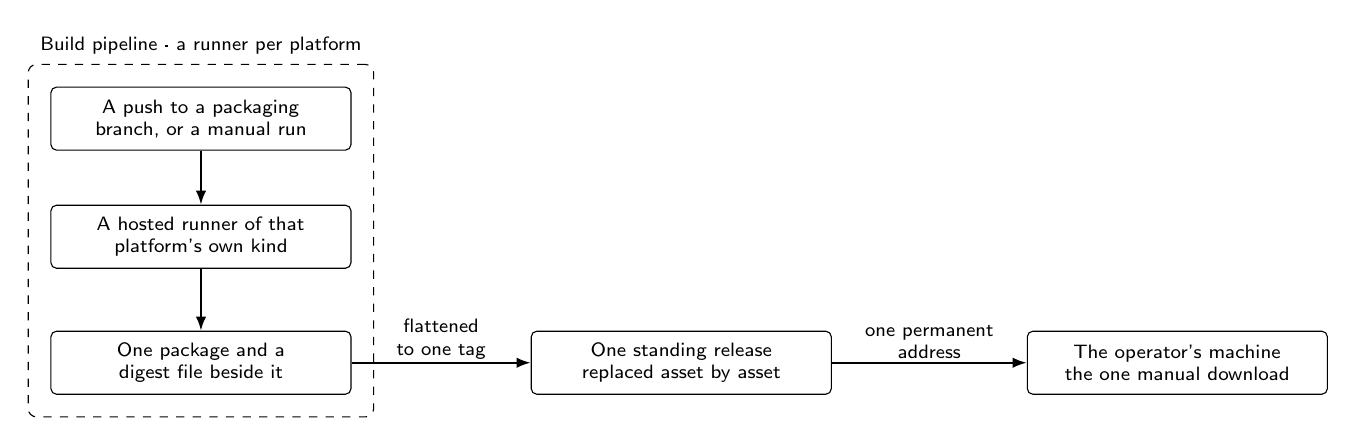
\begin{tikzpicture}[
    every node/.style={font=\scriptsize\sffamily},
    box/.style={
        draw,
        rounded corners=2pt,
        align=center,
        inner sep=3pt,
        minimum height=8mm,
        fill=white
    },
    lbl/.style={font=\scriptsize\sffamily, align=center,
        fill=white, inner sep=1pt}
]
    % Pipeline column x=2.7 (trigger, runner, artifact at 1.5cm and
    % 1.6cm pitch) · hand-off row y=-0.6 runs release x=8.8 then
    % operator x=15.1. Boxes are 3.6cm of text, 3.81cm drawn; the two
    % labelled corridors are 2.01cm and 2.49cm against labels 1.66cm
    % and 2.10cm wide, so no label touches the frame edge. Every run
    % is straight: two vertical in the column, two horizontal along
    % the row, none elbowed.
    \node[box, text width=3.6cm] (trig) at (2.7,2.5)
        {A push to a packaging\\branch, or a manual run};
    \node[box, text width=3.6cm] (run) at (2.7,1.0)
        {A hosted runner of that\\platform's own kind};
    \node[box, text width=3.6cm] (art) at (2.7,-0.6)
        {One package and a\\digest file beside it};

    \node[box, text width=3.6cm] (rel) at (8.8,-0.6)
        {One standing release\\replaced asset by asset};
    \node[box, text width=3.6cm] (op) at (15.1,-0.6)
        {The operator's machine\\the one manual download};

    \begin{scope}[on background layer]
        \node[archhost, fit=(trig)(run)(art),
            label={[archlabel]above:Build pipeline · a runner per platform}]
            (pipe) {};
    \end{scope}

    \draw[archflow] (trig.south) -- (run.north);
    \draw[archflow] (run.south) -- (art.north);
    \draw[archflow] (art.east) --
        node[lbl, above] {flattened\\to one tag} (rel.west);
    \draw[archflow] (rel.east) --
        node[lbl, above] {one permanent\\address} (op.west);
\end{tikzpicture}%
}
\caption{How one change becomes the one file an operator downloads.}
\label{fig:arch-delivery}
\end{figure}

Carrying a change to an operator is a push rather than a rebuild on
a workstation, and no developer machine stands in this path at all
(NFR-10). One packaging branch serves each desktop platform, and a
change pushed to it rebuilds that platform's package on a hosted
runner of the same kind of operating system, which is what a native
executable demands of the machine that builds it. The same build can
also be started by hand, for one platform or for both, when a
package is wanted ahead of any change. The two platforms are built
from one source tree by one recipe, so their files differ in
envelope rather than in contents, and each is published with a
digest beside it.

What is published is one standing release rather than a numbered
series. Each build replaces the asset already on that release in
place, so an operator is given a single address that always holds
the current build, and no version has to be numbered by hand or
redrawn when a build is repeated. The cost belongs to the same
picture: no earlier build is kept, so a return to a previous state
means rebuilding the branch it came from. Downloading the file is
the one step here that a person performs.

\section{Relation to Following Chapters}
\label{sec:arch-roadmap}

The figures in this chapter are the map of the system.
The next chapters zoom into each concern without
repeating the same overview diagrams:

\begin{itemize}
    \item Chapter~\ref{ch:monitoring} details the
    monitoring application: architecture, interaction
    with the gateway for installation and device
    onboarding, and operational workflows---building on
    Figures~\ref{fig:arch-monitoring},
    \ref{fig:arch-planes}, and~\ref{fig:arch-secrets}.
    \item Chapter~\ref{ch:gateway} details the gateway:
    agent and MQTT handling, the inbound processing path,
    APIs and control interfaces, and detection and
    response---building on
    Figures~\ref{fig:arch-gateway} and
    \ref{fig:arch-datapath}.
    \item Chapter~\ref{ch:encryption} details transport
    and application-layer protection: the mutual TLS
    handshake that admits a session, and the
    encrypt/decrypt workflow---building on
    Figure~\ref{fig:arch-protection}.
\end{itemize}
\chapter{Monitoring Application}
\label{ch:monitoring}

% Operator-PC runtime. Broader sections: architecture,
% how the app interacts with the gateway, and functions
% as workflows. Sources: architecture.md §2/§6,
% knowledge base §4.1--4.2 and §5.

This chapter details the monitoring application: the packaged
desktop runtime on the operator PC through which an operator
installs the local observability stack, provisions gateways over
the plant network, registers sensors on them, and reads host
health and inbound transmission activity. It covers three
concerns.

\begin{itemize}
    \item \textbf{Architecture of the runtime}
    (Section~\ref{sec:monitoring-architecture}).
    The processes the package starts, the control service behind
    the interface, and the local state the interface reads.
    \item \textbf{Interaction with the gateway}
    (Section~\ref{sec:monitoring-interaction}).
    How a host found on the network becomes a managed gateway,
    and how real and laboratory sensors become known to it.
    \item \textbf{Functions and operational workflows}
    (Section~\ref{sec:monitoring-functions}).
    Preparing the local stack, reading metrics and transmission
    activity, control and laboratory exercise, and the lifecycle
    of the installation.
\end{itemize}

\section{Architecture of the Monitoring Application}
\label{sec:monitoring-architecture}

The monitoring application is the operator-facing runtime of
IoT-SecureGate. A single native package combines three facilities:
\begin{itemize}
    \item An interface through which the administrator provisions gateways and observes operation
    \item A control service that performs every action directed at a gateway
    \item A local observability stack that receives gateway metrics and logs
\end{itemize}
This section describes the processes that make up that runtime, the division of
responsibility between them, the state the application keeps on
the operator PC, and the way the observability stack is installed
and configured.

\subsection{Process layout}
\label{sec:mon-processes}

The application is delivered as one package per platform, a
Windows executable or a Linux AppImage, and the administrator runs
a single program rather than assembling services from a repository
(NFR-1, NFR-2). A launcher acts as the process manager and starts
the two servers behind the interface. The wizard server, on port
9138 of the PC's own loopback address, serves the interface, answers
the setup steps that belong to it alone, and keeps unapplied form
edits until they are confirmed. The control service, on port 9137 of
the same address, is the program that owns the record of what is
under management, the privileged sessions toward gateways, and the
readings that the views display. Requests that the interface issues
for control work are passed to that service by the wizard server, so
the interface has no independent path to a gateway. A native window
presents the interface and displays a splash screen while the back
end reaches readiness. Figure~\ref{fig:mon-processes} shows these
processes together with the state each one writes.

\begin{figure}[htbp]
\centering
\resizebox{\textwidth}{!}{%
\begin{tikzpicture}[
    every node/.style={font=\scriptsize\sffamily},
    box/.style={
        draw,
        rounded corners=2pt,
        align=center,
        inner sep=3pt,
        minimum height=8mm,
        fill=white
    },
    lbl/.style={font=\scriptsize\sffamily, fill=white, inner sep=1pt}
]
    % Launch layer
    \node[box, text width=13.0cm] (shell) at (0,3.2)
        {Desktop shell\\launcher (process manager) · GUI host};

    % The two loopback servers
    \node[box, text width=4.2cm] (wiz) at (-3.0,1.8)
        {Wizard server\\port 9138 · SSH discovery};
    \node[box, text width=4.2cm] (ctrl) at (3.0,1.8)
        {Control service\\port 9137 · day-2 control};

    % Managed observability listeners
    \node[box, text width=13.0cm] (tele) at (0,0.0)
        {Local observability installed with the application\\
         Loki port 3100 · Prometheus port 9090 · Grafana port 9140};

    % Local state
    \node[box, text width=3.8cm] (reg) at (-4.6,-2.7)
        {Local registry\\gateways · devices};
    \node[box, text width=3.8cm] (key) at (0,-2.7)
        {OS keyring\\CA · sudo · PIN};
    \node[box, text width=3.8cm] (data) at (4.6,-2.7)
        {Application data\\settings · drafts};

    % The launcher starts both servers; the interface reaches the
    % control service through the wizard proxy
    \draw[archflow] (shell.south) -- (0,2.5) -- (-3.0,2.5) -- (wiz.north);
    \draw[archflow] (shell.south) -- (0,2.5) -- (3.0,2.5) -- (ctrl.north);
    \draw[archflow] (wiz.east) -- node[lbl, above] {proxy} (ctrl.west);

    % The setup side installs and configures the local stack; the
    % control service only reads measurements back out of it
    \draw[archflow] (ctrl.south) --
        node[lbl, right, pos=0.5] {query}
        (tele.north -| ctrl.south);
    \draw[archflowsoft] (wiz.south) --
        node[lbl, left, pos=0.5] {install · configure}
        (tele.north -| wiz.south);

    % Local state, fed from a trunk routed clear of the stack
    \draw (shell.east) -- (7.1,3.2) -- (7.1,-1.3);
    \draw[archflow] (7.1,-1.3) -- (4.6,-1.3)
        -- node[lbl, right, pos=0.5] {settings} (data.north);
    \draw[archflow] (7.1,-1.3) -- (0,-1.3)
        -- node[lbl, right, pos=0.5] {secrets} (key.north);
    \draw[archflow] (7.1,-1.3) -- (-4.6,-1.3)
        -- node[lbl, right, pos=0.5] {records} (reg.north);
\end{tikzpicture}%
}
\caption{Processes, state, and observability listeners of the
monitoring application.}
\label{fig:mon-processes}
\end{figure}

Network exposure differs by function, and the difference follows
from which side initiates the connection. The wizard server and
the control service bind to the PC's own loopback address and cannot
be reached from the plant network. The observability processes face
the opposite direction. Loki listens on port 3100 because the
gateway shipper pushes accepted log lines toward the operator PC,
and the application can add the corresponding inbound firewall
rule on Windows when it is run with elevation. Prometheus listens
on port 9090 and initiates scrapes toward each gateway, while
Grafana serves only the local browser and therefore binds port 9140
of the loopback address. None of these listeners authenticates
peers of its own, which is why they depend on the trusted-network
condition of NFR-9.

Responsibility for the two directions of gateway contact is split.
Everything that turns a host into a gateway belongs to the wizard
server: it scans the monitoring subnet for hosts offering SSH on port
22, pins the host key of the chosen host, installs an operator public
key using the one-time password offered for that step alone, and then
drives the installation over the session that key establishes,
recording the host as managed once the install reports healthy. Every
change made to a gateway after that point belongs to the control
service, applied over a session of the same kind. Broker configuration
is consequently never edited by hand: registration applies MQTT
credentials, topic permissions, a client certificate and a Kafka
topic programmatically, which is the form FR-6 requires.

\subsection{Inside the control service}
\label{sec:mon-modules}

The control service divides the work it owns into roles that answer
to the administrator's areas of responsibility. Two duties commonly
credited to it belong to the wizard server instead: preparing this
machine for monitoring, and admitting a newly discovered host as a
gateway. Each role below owns one kind of decision, and
Table~\ref{tab:mon-modules} states which one.

\begin{table}[H]
\centering
{\small
\begin{tabularx}{\textwidth}{@{}p{3.4cm}Y@{}}
\toprule
\textbf{Role} & \textbf{The decision it owns} \\
\midrule
Admitting a device &
Whether a sensor becomes managed at all: the credential it
connects with, the topics it may use, the certificate that
identifies it, and the stored stream reserved for its data---and the
withdrawal of all four when the device is removed. \\
\midrule
Controlling publication &
Whether an admitted device may publish at this moment; whether a
source that keeps sending invalid traffic should be cut off by the
gateway itself; and whether a device's stored history is emptied
while its place in the system is kept. \\
\midrule
Renewing trust material &
Whether the gateway can go on signing device certificates after its
signing material, or its own listener certificate, has to change. \\
\midrule
Answering the views &
What Metric and Activities are able to show. The questions they ask
are written down once here and answered from the local metrics and
log store, so a view never holds a query of its own. \\
\midrule
Changing a gateway &
The privileged edits after installation: who may connect, what each
device may publish, which stored streams exist, and with what
material a device's messages are to be opened. \\
\midrule
Feeding laboratory certificates &
Whether a simulated device still presents a valid certificate as it
runs, so that a test of the admission path remains a test of the path
rather than an exception to it
(Section~\ref{sec:monitoring-fakes}). \\
\bottomrule
\end{tabularx}}
\caption{The work the control service divides itself into, and the
decision each part owns.}
\label{tab:mon-modules}
\end{table}

Two boundaries follow from this division. Once a host is under
management, changes to its configuration are applied only by the
admitting and changing roles, over a session authenticated with the
key the setup steps installed, so that neither a view nor a manual
action can edit a gateway behind the application's back. Reads of
gateway behaviour reach the interface only through this service: the
Metric and Activities views do not contact Prometheus, Loki, or Kafka
directly. Grafana does query those sources, and is therefore opened
in the system browser as a separate tool rather than embedded in the
application.

\subsection{State on the operator PC}
\label{sec:mon-state}

The state the application keeps is summarised in
Table~\ref{tab:mon-state}. It separates three things: what the
application is allowed to operate on, what it can prove, and what it
merely remembers for convenience.

\begin{table}[H]
\centering
{\small
\begin{tabularx}{\textwidth}{@{}p{3.9cm}Yp{4.0cm}@{}}
\toprule
\textbf{State} & \textbf{What it decides} & \textbf{Who establishes it} \\
\midrule
Registry of what is managed &
Which hosts and devices the application may act on at all, and the
history of the changes made to them. &
The wizard server enters a gateway once its install reports healthy;
the control service enters every device and records each change after
that. Nothing unprovisioned can be operated on. \\
\midrule
Connection settings &
How a gateway is reached, and how the interface presents itself. &
The setup steps and the control service. No passphrase or password is
held here. \\
\midrule
Secrets &
Whether device certificates can be signed, whether a privileged
change can be applied on a gateway, and whether this console may be
opened at all. &
Written once when an install succeeds, then supplied automatically to
later requests. Never recorded among the settings or the logs
(FR-14, NFR-6). \\
\midrule
Unapplied form edits &
What the simulator forms show again when the operator returns to
them. &
The interface, retained across tab switches and restarts. Nothing on
a gateway changes until these are confirmed. \\
\midrule
Observability programs &
Whether this machine is ready to monitor anything, and on which
versions. &
The application, which obtains pinned versions once, at first run
(FR-13). \\
\bottomrule
\end{tabularx}}
\caption{State the monitoring application keeps.}
\label{tab:mon-state}
\end{table}

The registry determines what the application is able to operate
on. The gateway selector offered to the administrator is built from
what has been registered, and gateway details recorded only among the
connection settings do not appear in the monitoring views, so the
gateways available for operation are exactly those that have been
provisioned successfully. Device registration, publish block and
allow, and the related changes made afterwards are recorded there as
well, which is what keeps the configuration history inspectable after
the fact (NFR-8).

Credentials are held apart from that state, in the operating system's
own secret store where one is available, with a private file standing
in where there is none. Three kinds are kept: the passphrase that
unlocks a gateway's certificate authority, which is what lets device
certificates be signed; the credential that lets a privileged change
be applied on that gateway; and the personal identification number
that guards this console. When a control request arrives without one
of the first two, the request is completed from what is stored, so an
operation that follows a successful install does not require the
administrator to type it again (FR-14). A privileged command on a
gateway receives its password over the session itself rather than as
part of a remote command line, which keeps it out of the recorded
settings and out of the logs (NFR-6).

\subsection{The local observability stack}
\label{sec:mon-telemetry}

Loki, Prometheus, and Grafana are not dependencies of the
installer. On first run, triggered from the wizard, the application
obtains the pinned release of each, checks the available disk space
against a preflight minimum of 2.5\,GiB, and starts the three
processes. Readiness of all three is the condition for a completed
install, and holding to a pinned release list keeps every delivered
installer on the same versions (FR-13).

Monitoring configuration is generated rather than written by hand.
Installing a gateway registers it as a scrape target addressed to the
metrics endpoint that the agent exposes on port 9139, under the one
job name the two runtimes agree on. That name is part of the contract
between them: a panel whose query names a job that Prometheus is not
scraping remains empty even when the agent answers a direct HTTP
request, so the application writes the target list as part of
installation instead of leaving it to manual configuration. Grafana
is provisioned with Prometheus and Loki datasources and with one
Kafka datasource per registered gateway, addressed through the
external listener of that gateway on port 9094; this listener is
unauthenticated and rests on the same trusted-network condition as
NFR-9. The Grafana HTTPS certificate is self-signed and is offered
for download from the settings section rather than imported into the
operating system trust store automatically, so extending trust
remains an explicit administrator action.

The runtime holds configuration and observability data, not
message content. Accepted payloads stay in the gateway log and in
gateway Kafka topics, together with whatever the shipper forwards
to Loki, and the gateway certificate authority stays on the
gateway: the operator PC retains the passphrase that unlocks it,
not the key itself.

\section{Interaction with the Gateway}
\label{sec:monitoring-interaction}

Two operations carry the application from a PC that monitors nothing
to a gateway that reports on a plant: the sequence that turns a host
found on the network into a managed gateway, and the sequence that
makes a sensor known to that gateway. Both are described here as
processes, from the action taken at the interface to the state the
remote host is left in.

\subsection{Gateway discovery and installation}
\label{sec:mon-install}

Installation begins with an address rather than with a search. The
administrator first records the network address of the PC itself, and
discovery refuses to run until one is set, because that address
decides two things at once: the range that will be probed, and the
destination the gateway will later be told to send its log lines to.
Discovery then attempts a connection to port 22 on every address in
that subnet, leaving the PC's own address out of the range, refusing
to widen the search past a /24 or past 256 addresses, and abandoning
any single address after 0.35 seconds. What comes back is a list of
hosts that accept SSH, with nothing claimed about them beyond that;
the choice among them belongs to the administrator, from the screen of
Figure~\ref{fig:mon-ui-gateway}.

\appshot{UI-to-find-and-register-gateways.png}
    {Discovery and installation Gateway UI}
    {fig:mon-ui-gateway}

Trust is settled before anything is installed. The application reads
the host key of the chosen address without authenticating and reports
its fingerprint, and the administrator pins it. That pin is a
precondition for every later step that carries a credential: a session
presenting a different key is refused rather than accepted with a
warning. The password offered for this step is then used once, to
append a generated operator public key to the account; the application
verifies that it can connect with the key alone, and the password is
discarded rather than retained (NFR-6). From here on the host is
reachable only by key, which is what lets the remaining steps run
unattended.

Nothing is sent to the host until two further credentials are in hand:
one that lets the application act with privileges there, since
installing packages and controlling services is privileged work, and a
passphrase for the certificate authority the gateway will run. Both
are demanded before the first command rather than discovered halfway
through an installation. The passphrase may be generated by the
application or typed in, and the value \emph{admin} is rejected
outright. Neither is ever placed on a remote command line: the
privileged one is written to the standard input of the command that
needs it, and the passphrase is offered to the signing step through a
file it reads, which keeps both out of the host's process listing and
out of the record the PC keeps (NFR-6).

The installation itself is a fixed sequence, set out in
Table~\ref{tab:mon-install}. The order carries the reasoning: what can
be checked without writing anything is checked first, material is
created before the step that consumes it, and the one component whose
absence still leaves a workable gateway is placed last and separately,
so that its failure is reported instead of undoing the rest. A stage
that fails stops the sequence with a message naming the stage, and a
retry begins from a clean copy of the software rather than from the
partly written one.

\begin{table}[H]
\centering
{\small
\begin{tabularx}{\textwidth}{@{}p{3.1cm}Yp{3.9cm}@{}}
\toprule
\textbf{Stage} & \textbf{What it establishes} & \textbf{If it fails} \\
\midrule
Space preflight &
Whether the destination holds at least 2\,GiB free before anything is
unpacked. &
Refuses at once; the host is left untouched. \\
\midrule
Broker placed &
A message broker able to carry sensor traffic for this host. &
Stops at that stage, before any configuration exists to undo. \\
\midrule
Trust material created &
An authority that will sign device certificates, a listener
certificate naming the host's own address, and an identity the host
uses to read its own broker. &
An existing authority is never overwritten: the original passphrase is
demanded instead, or the host is removed first. \\
\midrule
Broker configured &
That clients are admitted only on port 8883 and only with a client
certificate, with per-device rules and credentials it can be pointed
at. &
Stops at that stage; the certificates already made stay inert. \\
\midrule
Storage budget prepared &
The accounting that later decides how many sensors the host may hold:
70 percent of its disk set aside for retained data, under a fixed
ceiling per stream. &
Stops; admission cannot be bounded without it. \\
\midrule
Stream storage &
The service that retains each device's accepted data. &
Deferred and reported. The rest of the installation stands, and the
capacity figures stay unknown until it succeeds. \\
\midrule
Agent placed and run &
The process that answers on port 9139 and ships activity toward the PC,
told at installation time which address to ship to. &
Stops; a retry starts from a clean copy rather than the partly written
one. \\
\bottomrule
\end{tabularx}}
\caption{The stages of installing a gateway.}
\label{tab:mon-install}
\end{table}

\begin{figure}[htbp]
\centering
\resizebox{\textwidth}{!}{%
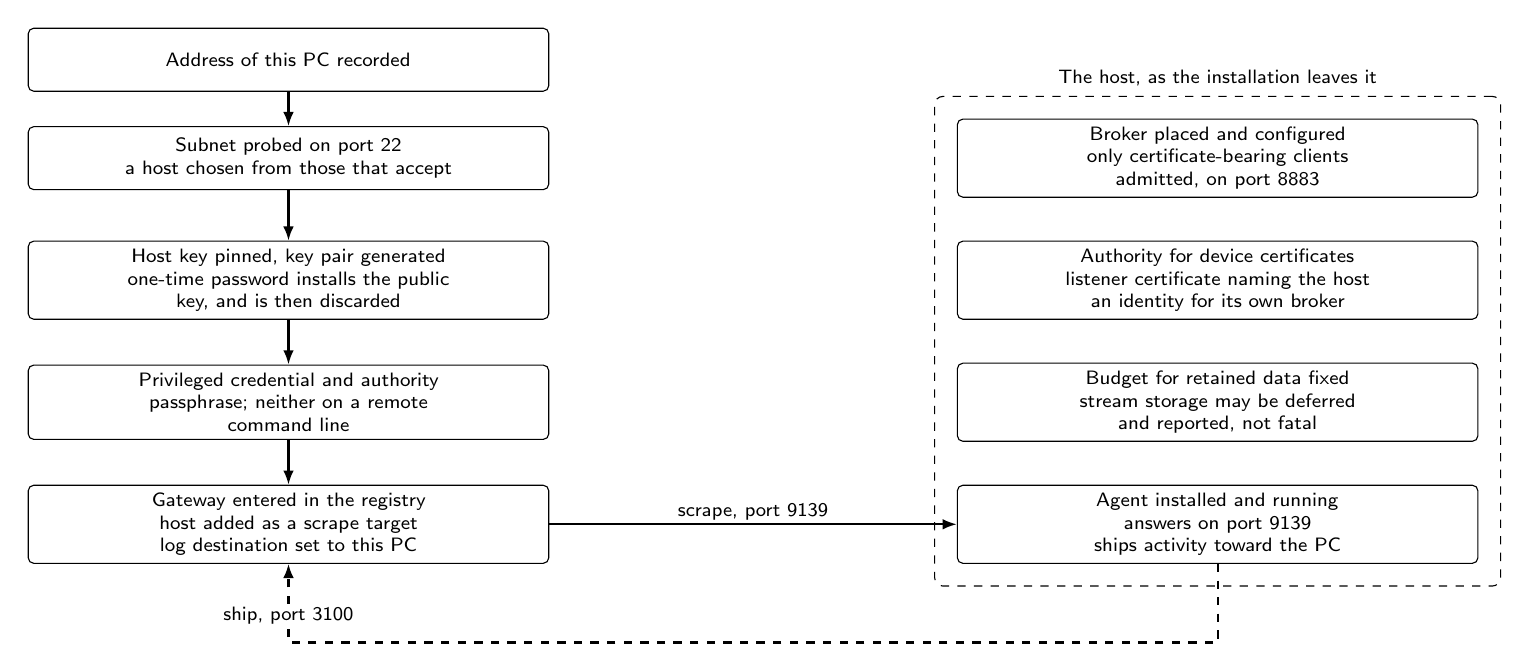
\begin{tikzpicture}[
    every node/.style={font=\scriptsize\sffamily},
    box/.style={
        draw,
        rounded corners=2pt,
        align=center,
        inner sep=3pt,
        minimum height=8mm,
        fill=white
    },
    lbl/.style={font=\scriptsize\sffamily, fill=white, inner sep=1pt}
]
    % Left lane = the operator's PC, right lane = the host, framed.
    % Lanes x=+-5.9 (text width 6.4cm, half-width 3.31cm).
    % Rows y: 4.90 · 3.65 · 2.10 · 0.55 · -1.00 (right lane starts one row
    % lower, so no two stacked three-line boxes sit closer than 0.32cm).
    % Every run is straight; only the return channel elbows, at y=-2.50.
    \node[box, text width=6.4cm] (addr) at (-5.9,4.90)
        {Address of this PC recorded};
    \node[box, text width=6.4cm] (scan) at (-5.9,3.65)
        {Subnet probed on port 22\\a host chosen from those that accept};
    \node[box, text width=6.4cm] (trust) at (-5.9,2.10)
        {Host key pinned, key pair generated\\
         one-time password installs the public\\
         key, and is then discarded};
    \node[box, text width=6.4cm] (creds) at (-5.9,0.55)
        {Privileged credential and authority\\
         passphrase; neither on a remote\\
         command line};
    \node[box, text width=6.4cm] (record) at (-5.9,-1.00)
        {Gateway entered in the registry\\
         host added as a scrape target\\
         log destination set to this PC};

    \node[box, text width=6.4cm] (broker) at (5.9,3.65)
        {Broker placed and configured\\
         only certificate-bearing clients\\
         admitted, on port 8883};
    \node[box, text width=6.4cm] (material) at (5.9,2.10)
        {Authority for device certificates\\
         listener certificate naming the host\\
         an identity for its own broker};
    \node[box, text width=6.4cm] (budget) at (5.9,0.55)
        {Budget for retained data fixed\\
         stream storage may be deferred\\
         and reported, not fatal};
    \node[box, text width=6.4cm] (agent) at (5.9,-1.00)
        {Agent installed and running\\
         answers on port 9139\\
         ships activity toward the PC};

    \begin{scope}[on background layer]
        \node[archhost, fit=(broker)(material)(budget)(agent),
            label={[archlabel]above:The host, as the installation leaves it}]
            (host) {};
    \end{scope}

    \draw[archflow] (addr.south) -- (scan.north);
    \draw[archflow] (scan.south) -- (trust.north);
    \draw[archflow] (trust.south) -- (creds.north);
    \draw[archflow] (creds.south) -- (record.north);

    \draw[archflow] (record.east) --
        node[lbl, above, pos=0.5] {scrape, port 9139} (agent.west);
    \draw[archflowsoft] (agent.south) -- (5.9,-2.50) -- (-5.9,-2.50)
        -- node[lbl, below, pos=0.5] {ship, port 3100} (record.south);
\end{tikzpicture}%
}
\caption{How a host becomes a managed gateway.}
\label{fig:mon-install-flow}
\end{figure}

The close of the sequence is what makes the host observable, and it is
FR-5 carried out in one action: the PC records its own address on the
gateway as the destination for shipped log lines, adds the host to the
set the local metrics collector queries, and enters it in the local
registry as a managed gateway, together with the credentials the next
operation will need (Section~\ref{sec:mon-state}). Readiness is judged
from inside the host, against its own loopback health endpoint, once a
second for up to fifteen attempts. Asking there rather than across the
network means a host firewall cannot manufacture a false failure, and a
reported success means the process came up rather than merely that the
installer finished. Figure~\ref{fig:mon-install-flow} shows what crosses
the session and what the host is left holding.

\subsection{Sensor and fake-sensor onboarding}
\label{sec:monitoring-fakes}

Before anything on a gateway is touched, admission asks how many more
sensors the host can hold. The answer comes from its disk: 70 percent
of total capacity is the budget for retained sensor data, each sensor
owns one stored stream with a ceiling of its own, and one gigabyte is
that ceiling by default, so a host with ten gigabytes of disk admits
seven sensors rather than ten. Total capacity is used deliberately
rather than free space: a budget that shrank as data accumulated would
refuse registrations for reasons the administrator could neither see
nor undo. A host already at its limit is refused before a file is
opened, and the refusal carries the figures behind it---the ceiling,
how many are admitted, how many places remain---which is what NFR-4
asks for and what makes the refusal actionable.

Admission then changes five things on the gateway, in an order arranged
so that the irreversible part comes last. A rule is added naming the
subjects this device may publish on, which by default covers both
halves of the split form the gateway expects to receive. A hashed form
of the connection password is merged into the credential file, and the
plaintext typed at the interface is erased once hashed. A key pair for
the device is generated on the PC and only the signing request travels,
so the private half is never exposed to the gateway. The stream
reserved at the capacity step is created with its ceiling attached. And
the material that will open this device's future messages, together
with the shape a message from it must have, is written on the host. The
broker is reloaded afterwards, so that the new rule and credential take
effect only once everything they refer to already exists. One form on
the PC is behind all five, and it is Figure~\ref{fig:mon-ui-register}.

\appshot{UI-to-register-sensor-for-gateway.png}
    {Registering a real sensor UI}
    {fig:mon-ui-register}

Two boundaries govern what happens when a step inside that list fails.
Until the reload, every write has a copy beside it and the whole action
is unwound, so a device that was not admitted leaves no half-written
rule, no orphaned credential line and no reserved stream. After the
reload the files stay, and the outcome is reported as degraded instead
of rolled back. The asymmetry is deliberate: the reload is the moment
the device becomes live, and restoring a saved copy of a running broker
could withdraw access from devices already publishing, which is a worse
fault than one the administrator can see and repair. The form itself is
checked before any session is opened, so a malformed identifier or
topic is reported as a mistake at the interface rather than as a
gateway failure. Figure~\ref{fig:mon-onboard} places that boundary on
the action itself.

\begin{figure}[htbp]
\centering
\resizebox{\textwidth}{!}{%
\begin{tikzpicture}[
    every node/.style={font=\scriptsize\sffamily},
    box/.style={
        draw,
        rounded corners=2pt,
        align=center,
        inner sep=3pt,
        minimum height=8mm,
        fill=white
    },
    lbl/.style={font=\scriptsize\sffamily, fill=white, inner sep=1pt}
]
    % One admission action, top to bottom, then the two kinds of device.
    % Main column x=0 (text width 13cm, half-width 6.61cm); refusal x=9.5.
    % Branch boxes x=+-3.65 (text width 6.4cm, half-width 3.36cm).
    % Rows y: 4.05 · 2.60 · 1.15 · -0.60 · -2.35 · -3.95.
    % Only the fork elbows, at y=-1.30; the two lower runs are straight
    % because they land on (both.north -| branch.south).
    \node[box, text width=13.0cm] (ask) at (0,4.05)
        {Register a sensor, or create a laboratory one};
    \node[box, text width=13.0cm] (gate) at (0,2.60)
        {Capacity first: 70 percent of the host's total disk\\
         divided by the ceiling held by one stored stream};
    \node[box, text width=3.6cm] (full) at (9.5,2.60)
        {Refused before anything\\is opened, with the\\figures included};
    \node[box, text width=13.0cm] (write) at (0,1.15)
        {Publish rule · hashed credential · signed certificate\\
         reserved stream · opening material and the message shape};
    \node[box, text width=13.0cm] (reload) at (0,-0.60)
        {The broker reload marks the boundary of the action---above it a failure\\
         unwinds every step; below it the files stay and later faults are reported};
    \node[box, text width=6.4cm] (real) at (-3.65,-2.35)
        {A real sensor: one download holding\\
         the broker's authority, its certificate\\
         and key, the material that opens its\\
         messages, and the shape they must have};
    \node[box, text width=6.4cm] (lab) at (3.65,-2.35)
        {A laboratory sensor: an address on a\\
         gateway-private test network, a unit\\
         stopped until started; certificates\\
         renewed with no operator in the loop};
    \node[box, text width=13.0cm] (both) at (0,-3.95)
        {Either way: port 8883, a password and a certificate presented together};

    \draw[archflow] (ask.south) -- (gate.north);
    \draw[archflowsoft] (gate.east) -- (full.west);
    \draw[archflow] (gate.south) -- (write.north);
    \draw[archflow] (write.south) -- (reload.north);
    \draw[archflow] (reload.south) -- (0,-1.30) -- (-3.65,-1.30)
        -- (real.north);
    \draw[archflow] (reload.south) -- (0,-1.30) -- (3.65,-1.30)
        -- (lab.north);
    \draw[archflow] (real.south) -- (both.north -| real.south);
    \draw[archflow] (lab.south) -- (both.north -| lab.south);
\end{tikzpicture}%
}
\caption{Device registration as a single action.}
\label{fig:mon-onboard}
\end{figure}

What comes back from a successful registration is one download holding
everything a sensor needs in order to connect and to be understood: the
certificate that authenticates the broker, the device's own certificate
and private key, the material its messages will be opened with, and the
shape it must publish in. That is the whole of FR-6 from the
administrator's side, and no broker file is ever edited by hand. The
registry keeps the certificate's fingerprint and expiry beside the
device, and every admission, refusal, block and allowance is recorded
there as well, so which devices are under management and what was done
to them stays inspectable afterwards (NFR-8). Re-admitting an identifier
that already exists is treated as a repair rather than as a second
device: the material is refreshed and the same stream reused, so no
second place is taken in the capacity budget. Removing a device releases
its credential, its rule and its stream together.

One field in the registration form deserves stating plainly. The
address given for a sensor is recorded for the operator's benefit; it
is not installed as a rule the broker enforces. Admission rests on the
password and certificate a device presents and on the topics it is
permitted to use, so a sensor that changes address carries stale
paperwork rather than different permissions.

Laboratory sensors follow the same admission path and then diverge in
ways that keep them honest as tests. Each is given an address of its
own on a private test network built on the gateway for the purpose, so
that a simulated device presents a peer address and a route of its own
instead of pretending to be the host it runs on. A service unit is
installed for it and deliberately left stopped: creating the device
makes it available, and only an explicit start makes it publish. Its
parameters---how often it publishes, on what subject, with what payload,
and which faults to introduce---are stored on the PC when applied and
pushed to the host, while edits that have not been applied survive a
restart of the interface. The form behind that arrangement is
Figure~\ref{fig:mon-ui-fake}.

\appshot{UI-to-create-fake-sensors-for-testing.png}
    {Creating a laboratory sensor UI}
    {fig:mon-ui-fake}

The divergence that matters for the security argument is the
certificate. A laboratory device cannot download a bundle, so the
control service renews and installs its material with no operator in
the loop: a pass runs at start-up and then every ten minutes, renewing
a certificate once it falls within the smaller of thirty days or a
tenth of its lifetime of expiry, and also whenever the material the
simulator holds no longer matches what the registry records. Two
settings are exempt from that repair. Where the operator has asked the
simulator to omit its client certificate or to present a wrong
one---the two faults that test admission itself---the automatic feed
stands aside until the setting is cleared, because silently fixing that
would silently cancel the test. And a host whose authority cannot be
unlocked is skipped for half an hour with a record, rather than retried
every ten minutes indefinitely. Both outcomes reach the same
configuration record as a manual change (NFR-8). Laboratory publishers
draw on the same capacity budget as real ones, so a test rig cannot
report room that the disk does not have (NFR-4).

From the gateway's side the two kinds converge. Both connect on port
8883, both present a password and a certificate, and from there their
messages take the same inward path.

\section{Functions and Operational Workflows}
\label{sec:monitoring-functions}

Day-to-day use of the monitoring application is four repeatable
processes:
\begin{itemize}
    \item Making this machine ready to monitor, once at first use and
    again on every later start
    \item Reading gateway health and inbound transmission activity
    \item Changing what an admitted device may do, and exercising the
    same path with laboratory sensors
    \item Maintaining the installation on this PC as its certificates,
    its delivery, and finally its removal come into question
\end{itemize}
Each is described below as a process rather than as a tour of the
interface: what it changes, in what order, and what it reports when a
step in the middle of it fails.

\subsection{Local monitoring preparation}
\label{sec:mon-localprep}

Preparing the machine is one action, reused. It opens by asking whether
the metrics collector, the log store, and the dashboard are already
answering; if all three are, the action ends there without obtaining
anything. The same action therefore serves the first run and every
start after a reboot, and once the installation is complete the panel
performs it on launch by itself, in the background, so that the
interface opens while the stack is still coming up. Nothing is
downloaded for a component that is already present, which is why a
preparation step that failed halfway is retried by pressing the same
control rather than through a separate repair path. The screen from
which it is driven is Figure~\ref{fig:mon-ui-prep}.

\appshot{Download-Start-Up-Screen.png}
    {The first-run screen}
    {fig:mon-ui-prep}

The path that skips the download still rechecks the one thing that
changes after the fact: which gateway the collector is pointed at.
Preparation normally runs before any gateway has been installed, so the
scrape target still names this machine, and the health view would stay
empty indefinitely; the target list is therefore rewritten whenever it
disagrees with what is registered, and if the collector is already
running it is asked to reload its configuration rather than restarted,
so that the readings already collected survive the change
(Section~\ref{sec:mon-telemetry}).

The ordering is guarded at each step. A component is started only when
neither the process the panel tracks nor a fresh probe reports it
running, so a second preparation cannot compete with the first.
Readiness is all three answering their own readiness endpoint, waited
for up to ninety seconds. Two failures are kept apart rather than
collapsed into one: an address already held by something that is not
the expected component is reported at once, naming the port, instead of
consuming the whole waiting window, and a component that dies after
being started is reported from its own output. Progress arrives as the
state of a background job that the interface polls, so a download
neither blocks the interface nor leaves it guessing.

One part of preparation belongs to the platform rather than to the
system. The log store on this PC accepts pushes from the gateway, so
the machine has to admit inbound connections for it; on Windows the
application applies exactly one rule for that port, and only from an
elevated process, refusing and naming the remedy where it is not
elevated, and deleting the rule before re-adding it so that applying it
twice is harmless. Confirmation is taken from the rule being present
rather than from an acknowledgement, so reopening the step after a
restart does not lose it. Where the operating system offers no such
facility, nothing is attempted and the equivalent instruction is shown
instead. The rule names a port and not a source range, so what bounds
that exposure is the trusted-network condition of NFR-9 rather than the
rule itself.

Preparation also leaves behind the material the dashboard needs: a
self-signed certificate generated on this machine, and a generated
administrator password in place of a vendor default. Its fingerprint
and expiry are shown on the settings area that offers the certificate
for download, which is where Section~\ref{sec:mon-lifecycle} returns to
it. The stack itself runs as ordinary processes on this PC, with no
container runtime anywhere in the operator path (FR-13, NFR-2).

\subsection{Observing metrics and transmission activity}
\label{sec:mon-views}

The two monitoring views differ in what they read, not in how they
look. Metric answers FR-7, the health of the host and of the five
components named there; Activities answers FR-8 and FR-9, what arrived
at the gateway, how fast, how late, and what was refused. Both work on
a chosen gateway over a chosen window, refreshed on request or on a
fifteen-second timer, and neither holds a question of its own: the
questions are written down once in the control service, which is the
only part of the operator path that puts them to the local collector
and log store (Section~\ref{sec:mon-modules}).

The host readings come from the gateway itself. The agent reports
processor, memory, disk, load, temperature, and network counters under
the names the panels already expect, so the gateway runs no separate
exporter for its own machine (NFR-3), and the liveness of each of its
components arrives in that same reading. The component list shown is
the one FR-7 fixes, in the order the pipeline runs them, and a
component that the last reading does not mention is shown down rather
than omitted: the shape of the view does not depend on what happened to
arrive, and Figure~\ref{fig:mon-ui-metric} is that view.

\appshot{UI-for-general-metric-reading-from-gateway.png}
    {Gateway Metrics Visualization UI}
    {fig:mon-ui-metric}

Where a figure can be obtained two ways, the agent's own counter is
preferred and counting shipped log lines is the fallback. The reason is
that the log route thins out precisely when traffic fails---a burst of
messages that never survives to be logged would make the view look
quiet at the worst possible moment---whereas the counter counts
accepted and refused attempts together and shows the volume either way.
The refusal total is taken as the larger of the available sources
rather than trusted to one, because an agent predating the widened
counter reports only the class of refusal it knows about and would
otherwise understate the whole.

The list of refused or invalid messages is read from the gateway's own
record of recent refusals rather than from the log pipeline: the
reason, the device, the source address, the moment of arrival, and the
gateway, partitioned so that one device's history can be read on its
own (FR-9). Where the gateway could not resolve a source address, the
address that device is registered with is filled in, so a row is not
anonymous merely because the broker could not say who sent it---which
matters because a source address is exactly what an automatic
restriction needs in order to act (Section~\ref{sec:mon-control}). The
view that sets these rows beside the aggregate figures is
Figure~\ref{fig:mon-ui-activities}.

\appshot{UI-for-visualize-activity-metric-from-gateway.png}
    {Gateway Activities Visualization UI}
    {fig:mon-ui-activities}

What the views do not do is infer their own subject. The sensor list
comes from the registry rather than from observed traffic, so a
registered device that has never connected is shown with zeroes and the
silence belongs to the device instead of being an absence from the
list; observed connection details are laid over those rows as an
overlay. A device may stay registered while being taken out of
monitoring: that choice is recorded on the device and reported beside
it, but it is not what removes a device from sight. The aggregate
figures come from the collector rather than from that list, so traffic
is still counted on a gateway where nothing has been registered yet.

Nothing in this path is allowed to fail the page. Each question to a
backend is bounded, and a failure becomes a warning beside a zero, so
an unreachable collector leaves a partly empty summary rather than an
error; the header state then distinguishes live, degraded because some
question failed, and no scrape, which is the collector's own verdict
that it has not reached that gateway. A gateway-side read that times
out leaves its table empty rather than repeating what it saw before. An
empty chart is therefore not silently ambiguous.

Two things escalate rather than wait to be read. New invalid messages,
or an active automatic quarantine, raise a banner on Activities and a
count on its navigation entry, kept current even while the operator is
on another page (FR-9). Dismissing records a moment in time rather than
switching the alarm off: any later invalid message reopens it, while a
quarantine holds the alarm on its own, because it is a state the
gateway is still in rather than an event that has passed. Such a trip
is learned from the gateway's report, mirrored onto the device's local
record, and cleared from that record by the release action rather than
by a later reading that happens not to mention it.

\subsection{Control and laboratory exercise}
\label{sec:mon-control}

Four actions change what an admitted device experiences: publication
may be withheld and restored, an automatic restriction may be armed
against it and released, its stored history may be emptied, and a
laboratory unit may be driven at the path. All four are applied over
the privileged session that installation established, and each leaves
an entry in the registry beside the device it touched, which is what
keeps a later reading of the configuration trustworthy (NFR-8).
Table~\ref{tab:mon-control} states the width of each: what it edits on
the gateway, and what it deliberately leaves standing.

\begin{table}[H]
\centering
{\small
\begin{tabularx}{\textwidth}{@{}p{3.6cm}Yp{4.2cm}@{}}
\toprule
\textbf{Action} & \textbf{What it edits on the gateway} &
\textbf{What it leaves alone} \\
\midrule
Withhold publication &
The permission to publish, replaced by a read-only floor; a laboratory
unit is stopped with it. &
Registration, password, certificate, reserved stream, topics. \\
\midrule
Restore publication &
The permission, from the topics noted when it was taken. &
Everything else; nothing new is created. \\
\midrule
Arm automatic restriction &
A rule of count and window that the gateway enforces on its own, and a
firewall drop of the source address once it trips. &
Standing at the broker; a laboratory unit keeps running. \\
\midrule
Release a quarantine &
The drop for the address recorded at the trip. &
The rule, which stays armed. \\
\midrule
Empty stored history &
The stored stream, deleted and recreated at the same ceiling. &
Registration, credentials, and the place held in the capacity budget. \\
\bottomrule
\end{tabularx}}
\caption{The four control actions and how far each one reaches.}
\label{tab:mon-control}
\end{table}

Withholding publication is narrow by design (FR-10). The device keeps
its identity and everything provisioned around it, so restoring it is
an edit to one permission rather than a fresh registration, and the
read-only floor left behind means that publication alone is what
breaks. The topics taken away are noted locally at the moment of the
action, so restoration gives back what was there rather than a default,
and a request to withhold from a device already silent is reported as
already done instead of as a failure. A laboratory unit is stopped as
part of the same action, because leaving it running would only generate
refusals against a permission that no longer exists.

The automatic restriction is armed as a rule and then left with the
gateway: a count of invalid messages and a window, within bounds the
application enforces, pushed to the host that has to apply them
(FR-11). Enforcement is therefore the gateway's own, and a panel that
is closed or disconnected does not disarm it. When the rule trips, the
source address is dropped at the gateway's firewall, so that traffic
stops reaching the broker at all rather than arriving to be refused;
the trip is reported back with its address, moment, limit, and count,
mirrored into the device's local record, and shown as one of three
states---off, armed, or quarantined. Two separations are deliberate:
saving an edited rule does not release a quarantine already in force,
and releasing one does not disarm the rule. Where a gateway lacks the
helper that performs a release, the action says so and says what to do
about it, clearing the stuck record on the host so that the rule can
arm again, rather than reporting a release it did not achieve. The
surface on which a rule is armed and a quarantine released is
Figure~\ref{fig:mon-ui-control}.

\appshot{UI-to-control-registered-sensors.png}
    {Publication control and automatic restriction UI}
    {fig:mon-ui-control}

Emptying a device's stored history deletes its stream and recreates it
with the same ceiling, so the capacity accounting of
Section~\ref{sec:monitoring-fakes} is undisturbed and the device keeps
its place. It is not a withdrawal; and where a gateway has no stream
storage at all, the refusal says that, rather than reporting a generic
failure.

The laboratory exercise drives the same path from the inside. A unit
carries its publish interval, topic, payload, and behaviour toggles;
confirming them writes the confirmed settings into the local record
first, pushes them to the gateway, and then restarts the unit. A
restart that fails is reported as settings saved here and there but not
running, and the device's record carries the fault: the two halves of
the action are reported apart rather than undone together, which is what
lets the operator retry the second half alone. Starting a unit also
enables it, so a laboratory device returns after its host is restarted,
which is what makes an unattended run meaningful.

Two consequences of those toggles are worth stating. Setting an
attack-like behaviour pauses automatic renewal of that device's
certificates, because renewing them would repair the very condition
under test, so an expired laboratory certificate during such a run is
the expected state and not a fault. And a quarantined laboratory unit
keeps running: the drop sits at the firewall, so the exercise continues
while its publishes stop arriving. That is what makes FR-11 observable
rather than merely enforceable, and the invalid traffic these toggles
produce is the traffic FR-9 requires to be surfaced and that NFR-5
keeps out of accepted storage.

\subsection{Lifecycle of the operator installation}
\label{sec:mon-lifecycle}

Three things about this PC age: the certificate the dashboard serves,
the packaged application itself, and the installation, when it is
eventually taken away.

The dashboard speaks HTTPS on a self-signed certificate generated here,
so a browser will complain until the operator chooses to trust it; the
certificate is offered for download and trust is extended by hand, with
the steps differing by platform, rather than arranged silently.
Regenerating it mints a new pair, rewrites the dashboard configuration
with the scrape target preserved, stops whatever holds the dashboard
port---including a listener left behind by an earlier elevated run that
the present process does not know as its own child---starts a
replacement, and reports success only after that replacement has become
healthy. The fingerprint and expiry are shown so that an operator can
tell one certificate from the next instead of guessing from a browser
warning.

The application is delivered as one native package per
platform and needs no container runtime or compatibility
layer on the PC (NFR-2); carrying a change to an operator is
the pipeline matter of Section~\ref{sec:arch-delivery} rather
than a rebuild on a workstation (NFR-10).
Within the delivered package, the same executable re-enters itself as
the child process that answers control requests, so no system runtime
is assumed at the far end; and the interface is embedded when the
package is built, which is why an interface change reaches an operator
only in a new build. The part of the interface that signs build output
is held behind a personal identification number of which the secret
store keeps a digest and never the number itself; unlocking yields a
session that expires after fifteen minutes, and five failed attempts
produce a thirty-second pause before further ones. Signing identities
and their passphrases live in the same store (FR-14, NFR-6).

Removal has two scopes, and they are not one action at two sizes.
Taking a single gateway away uninstalls its agent over the session that
installed it, using that gateway's own stored privileged credential and
asking only where none was saved, then drops the registry row and the
credentials held for it. Where the key or the login name is missing, the
action says so and offers the narrower alternative---the local row can
be dropped, but the host keeps its software---instead of reporting a
removal that did not happen.

Removing the panel is deliberately wider. It implies every gateway
registered to it; it then stops the dashboard first, so that its files
stop being held, stops the rest, sweeps any listener left on those
ports by an earlier session, removes the downloaded programs with their
configuration and collected data, clears the credentials held here
including the fallback file that stands in where the system store was
unavailable, and finally wipes the local application data---which is
also what returns the panel to the preparation step of
Section~\ref{sec:mon-localprep}. Two properties matter more than the
list. Removal is idempotent, so a tree that is already gone counts as
success and the action can be repeated after a partial one; but a file
that could not be removed is named, and the result is marked as not
clean rather than the wipe being called complete. And a gateway that can
no longer be reached does not block removal of the panel: it is
reported, and the local state is cleared anyway, because the alternative
would be a machine that cannot be decommissioned.

\chapter{Gateway}
\label{ch:gateway}

% Edge runtime without a deep encryption chapter here.
% Focus: what the gateway handles, how the agent works,
% APIs that expose/control that work, and detection/response.
% Encryption/decryption: Chapter~\ref{ch:encryption}.
% Sources: architecture.md §3--4, knowledge base §4.3--4.4,
% details.md (ports/APIs).

This chapter details the gateway: the edge runtime that decides
which devices may publish, what they may publish, and what becomes
of the traffic that reaches it. On one small host it admits
sensors, authorizes each publish, recovers and validates the
content of what was accepted, stores the result for internal
consumers, and keeps the whole path observable and restrictable
from the operator PC. It covers five concerns.

\begin{itemize}
    \item \textbf{Architecture of the gateway}
    (Section~\ref{sec:gateway-architecture}).
    The service units on the host, the working roles inside the
    agent process, and the state the gateway keeps.
    \item \textbf{Agent operation and MQTT handling}
    (Section~\ref{sec:gateway-agent}).
    What the broker decides at connect and at publish, the agent's
    standing as a client of that broker, and the handling of a
    delivery inside the agent.
    \item \textbf{Inbound processing path}
    (Section~\ref{sec:gateway-inbound}).
    One publish placed in the full order of the path, from delivery
    to the two storage sinks and the hooks that make each stage
    observable.
    \item \textbf{Gateway APIs and control interfaces}
    (Section~\ref{sec:gateway-apis}).
    The HTTP surface the agent exposes and the control actions that
    change gateway state.
    \item \textbf{Detection and response behaviour}
    (Section~\ref{sec:gateway-detection}).
    What the gateway is able to notice about a transmission, denied and
    invalid traffic as gateway behaviour, and the two ways a device is
    restricted.
\end{itemize}

Message protection on this path---the transport layer and the
application-layer envelope that the agent opens---is treated
separately in Chapter~\ref{ch:encryption}.

\section{Architecture of the Gateway}
\label{sec:gateway-architecture}

The gateway is one host running three service units: 
\begin{itemize}
    \item a broker that admits sensors and authorizes their publishes
    \item a messaging storage service that internal consumers read
    \item the agent---a single process that recovers and checks what was admitted and exposes the state of the rest of the host
\end{itemize}
This section describes those units,
the roles the agent divides its work into, and the state the whole
path depends on.

Five requirement groups constrain that shape.

\begin{itemize}
    \item \textbf{NFR-3.}
    The runtime must run as services on a Raspberry Pi--class
    host, which rules out a container runtime on the device and
    leaves one Java process, the Kafka broker, as the only
    substantial non-Python component.
    \item \textbf{FR-1 and FR-2.}
    Admission and authorization are decided at the broker, so the
    host presents a single authenticated ingress rather than
    several.
    \item \textbf{FR-4 and NFR-4.}
    Accepted data goes to two sinks, and the number of devices
    those sinks can serve is bounded by the disk of one small
    machine.
    \item \textbf{FR-7 and FR-8.}
    Host health and inbound activity must be reachable over HTTP
    from the operator PC during ordinary operation.
    \item \textbf{FR-12.}
    The same host must generate laboratory traffic for testing
    without weakening the path that real sensors use.
\end{itemize}

\subsection{Service units}
\label{sec:gw-units}

The delivered gateway is three services on the host, plus an
optional fourth that exists only on a gateway used for laboratory
work.

\begin{itemize}
    \item \textbf{Message broker} (\texttt{mosquitto.service}).
    The distribution's own broker service, enabled and configured by
    the installation step rather than replaced by a component of this
    project. It owns sensor ingress on MQTTS port~8883, where a
    client must present both a credential and a client certificate
    chaining to the gateway CA before the connection is accepted
    (FR-2).
    \item \textbf{Gateway agent} (\texttt{iot-gateway-agent}).
    The platform's own runtime: one process that does everything
    described in this chapter. It runs against the broker that
    already exists on the host instead of starting one, restarts on
    failure after a three-second pause, and is ordered behind the
    broker so that the broker is expected to listen by the time the
    agent begins to connect.
    \item \textbf{Message storage} (\texttt{iotgw-kafka}). Apache
    Kafka in single-node KRaft mode, held to a memory budget of
    128--256\,MB: the constraint that keeps a messaging tier
    practical on the modest host NFR-3 assumes.
    \item \textbf{Laboratory publisher}
    (\texttt{iotgw-fake@\textless device\_id\textgreater}).
    One service per laboratory fake sensor (FR-12), each running its
    publisher inside a private network of the gateway's own, so that
    a simulated device holds an address like a real one. It reaches
    the broker over MQTTS like any other publisher, which is what
    makes it a test of the admission path rather than a bypass around
    it. Registration installs it stopped, and the operator starts it
    only when running the simulator (Chapter~\ref{ch:monitoring}).
\end{itemize}

The decision to run the agent against the broker that already exists
on the host is the load-bearing one in this layout. The agent can
alternatively configure and supervise a broker of its own, and that
path is what a developer uses when working from a source tree; the
delivered gateway does not use it. The consequence matters for the
security argument, because it makes the agent a \emph{client} of the
broker rather than its owner. It connects back to the broker over the
loopback address as an ordinary MQTT client holding a certificate of
its own, and subscribes to the whole sensor topic tree. Every message
the agent ever processes was therefore delivered to it by a broker
that had already applied the authentication and topic-authorization
checks FR-2 requires, and no message that the broker refused is
visible inside the agent. A rejected connect or an unauthorized
publish enters the agent's world only later, as a line in a broker
log that a separate role reads. Section~\ref{sec:gateway-detection}
returns to that split, because it is the reason the denial counts and
the message counts are two different measurements rather than one.
Figure~\ref{fig:gw-processes} draws the pieces together, with the
state they read and the two links that leave the host. Accepted records are kept on this host and read from there, and the
read is a third way anything leaves: the operator's reader takes them
straight off the storage listener from the plant network, as
Figure~\ref{fig:arch-topology} draws.

\begin{figure}[htbp]
\centering
\resizebox{\textwidth}{!}{%
\begin{tikzpicture}[
    every node/.style={font=\scriptsize\sffamily},
    box/.style={
        draw,
        rounded corners=2pt,
        align=center,
        inner sep=3pt,
        minimum height=8mm,
        fill=white
    },
    lbl/.style={font=\scriptsize\sffamily, fill=white, inner sep=1pt}
]
    % main.py + decrypt_worker.py + shipper.py: one host, ingress on top, the
    % agent frame holding the working roles, state kept beneath it.
    % Rows: ingress 4.7 · broker/storage 2.9 · roles 0 · state -2.9
    % Operator column x=9.9 (Prometheus 0 · Loki -1.7) · push rail y=-1.7
    % Arrows are straight runs aligned by coordinate intersection; only the
    % Loki line elbows, at y=-1.7.
    % Layer 1: publishers. Layer 2: the two peer services.
    \node[box, text width=13.2cm] (ingress) at (0,4.7)
        {Sensor ingress\\registered sensors over the plant LAN ·
         optional laboratory publisher};

    \node[box, text width=5.9cm] (mosq) at (-3.8,2.9)
        {Mosquitto broker\\MQTTS, port 8883 · client certificate\\
         password · per-device topic rules};
    \node[box, text width=5.9cm] (kafka) at (3.8,2.9)
        {Kafka storage (KRaft)\\internal, on localhost port 9092\\
         external, gateway address port 9094};

    % Layer 3: one process, four working roles
    \node[box, text width=3.9cm] (dpath) at (-4.6,0)
        {consume and open\\recover · validate\\accept or refuse};
    \node[box, text width=3.9cm] (detect) at (0,0)
        {denial capture\\broker refusals\\invalid records};
    \node[box, text width=3.9cm] (serve) at (4.6,0)
        {ship and report\\Loki push · HTTP port 9139};

    \begin{scope}[on background layer]
        \node[archhost, fit=(dpath)(detect)(serve),
            label={[archlabel]above:%
                Gateway agent · one process · four working roles}]
            (agent) {};
    \end{scope}

    % Layer 4: state kept on the host. Right column: operator peers.
    \node[box, text width=13.2cm] (files) at (0,-2.9)
        {State kept on the host\\admission identities and topic rules,
         read by the broker\\per-device message material, read by the
         agent\\accepted sensor data and refusal records, appended as
         traffic arrives};

    \node[box, text width=2.9cm] (prom) at (9.9,0)
        {Operator\\Prometheus\\port 9090};
    \node[box, text width=2.9cm] (loki) at (9.9,-1.7)
        {Operator\\Loki\\port 3100};

    % Ingress to broker to agent, and the agent's one produce
    \draw[archflow] (ingress.south -| mosq.north) --
        node[lbl, left, pos=0.5] {MQTTS} (mosq.north);
    \draw[archflow] (mosq.south) --
        node[lbl, left, pos=0.35] {only what it admits}
        (agent.north -| mosq.south);
    \draw[archflow] (agent.north -| kafka.south) --
        node[lbl, right, pos=0.65] {one stream per device}
        (kafka.south);

    % Observability leaves the host on these two links; accepted records
    % leave too, read off storage from the plant network (fig:arch-topology)
    \draw[archflowsoft] (agent.east) --
        node[lbl, above, pos=0.5] {scrape} (prom.west);
    \draw[archflowsoft] (serve.south) -- (4.6,-1.7)
        -- node[lbl, above, pos=0.5] {push lines} (loki.west);
    \draw[archflow] (agent.south -| dpath.south) --
        node[lbl, right, pos=0.5] {read · append}
        (files.north -| dpath.south);
\end{tikzpicture}%
}
\caption{The gateway runtime as deployed, and the state the host keeps.}
\label{fig:gw-processes}
\end{figure}

\subsection{Inside the agent process}
\label{sec:gw-agent-process}

The agent is a single process carrying four working roles, plus one
component that is consulted rather than run.

\begin{itemize}
    \item \textbf{Consume and open.}
    The role that holds the connection to the broker described
    above. It receives what the broker delivers, recovers the
    content of each message, checks the result against the rule that
    device was registered under, and decides whether the message is
    accepted.
    \item \textbf{Incomplete-message cleanup.}
    A protected message arrives in two parts that may come in either
    order. This role discards a part whose partner never arrived, so
    an unfinished message becomes a recorded refusal with a reason
    rather than something held in memory indefinitely.
    \item \textbf{Denial capture.}
    The role that reads the broker's own log and turns refusals into
    the counts and records an operator sees
    (Section~\ref{sec:gateway-detection}).
    \item \textbf{Shipping and reporting.}
    The role that forwards accepted records to the operator's log
    store, together with the interface that answers health and
    metric requests from the operator PC.
    \item \textbf{Restriction policy.}
    Auto prevent is consulted rather than run: it holds the window
    of recent invalid messages and the quarantine decision, is
    offered to whenever a refusal is recorded, and is read on request
    (Section~\ref{sec:gateway-detection}).
\end{itemize}

Running these roles in one process is what makes their shared state
cheap. The counters that feed the Activities view are produced by
the role that accepts messages and read by the reporting role in the
same place; a refusal is at the same moment an alert for the
operator, an input to the restriction window, and an entry the
operator can query later. Nothing has to cross a process boundary,
and the failure behaviour stays legible: one service, one restart
policy, one log to read.

The cost is equally plain. A fault in any role stops the whole
process, including the interface that would report the fault, and
there is no peer service on the device to restart it. The layout
accepts that because the outcome an operator observes is the same
either way---the Metric view shows the gateway and its consume role
as down---and because repair is an operator action over the control
plane rather than an on-device supervisory loop.

What an operator sees of these roles is their state, presented in
the Metric view in a fixed order: Agent, MQTT, Decrypt, Shipper,
Kafka. That order is a dependency chain rather than an arbitrary
list, and each state is derived from the thing it depends on. The
gateway itself is up whenever the process answers. Decrypt
and Shipper are up when their roles are running. MQTT is up when the
broker accepts connections on its configured port, which is how a
broker maintained as an independent service is judged. Kafka is up
when the storage service answers. The chain reads in the direction
of consequence: with the broker down there is nothing to consume,
and with nothing consumed there is nothing to ship. Those states
reach the operator through the metrics scrape and not through the
administrative session, so the separation drawn in
Chapter~\ref{ch:architecture} holds during an outage and not only in
ordinary operation.

\subsection{State the gateway keeps}
\label{sec:gw-state}

What the gateway must remember falls into a small number of kinds,
and the distinction that matters is not where each is kept but who
establishes it. Everything that decides admission or recovery is
placed by the operator's control plane as part of registration,
which is what FR-6 requires in practice: a device gains a right to
publish only through an action that also leaves a record in the
operator's registry (NFR-8). Everything the gateway learns by
handling traffic is its own output. Table~\ref{tab:gw-state}
separates the two.

\begin{table}[H]
\centering
{\small
\begin{tabularx}{\textwidth}{@{}p{3.9cm}Yp{4.0cm}@{}}
\toprule
\textbf{State} & \textbf{What it decides} & \textbf{Who establishes it} \\
\midrule
Admission identity &
Whether a client may connect at all, and which topics it may publish
to. &
The control plane, at registration; removed again at unregistration.
Replaced as a whole rather than edited in place, so the broker never
acts on a half-written rule set. \\
\midrule
Message material &
Whether the content of an admitted publish can be recovered, and
what shape the recovered message must have. &
The control plane, at registration. The day-scoped part is created
and renewed by the gateway itself (Chapter~\ref{ch:encryption}). \\
\midrule
Capacity reservation &
How many more devices this host can hold, and which device owns
which stored stream. &
The control plane, checked against the host's remaining disk before
a device is admitted. \\
\midrule
Accepted data &
The record of what the gateway took in, read by internal consumers
and forwarded to the operator's log store. &
The gateway, as traffic arrives. \\
\midrule
Refusal records &
What was denied or judged invalid, and the running count behind
automatic restriction. &
The gateway, as traffic is refused. \\
\midrule
Laboratory addresses &
Which simulated device holds which address on the gateway's own test
network. &
The control plane at creation, re-established whenever the simulated
device is started. \\
\bottomrule
\end{tabularx}}
\caption{State the gateway keeps, what each kind decides, and who
establishes it.}
\label{tab:gw-state}
\end{table}

The reservation row is where NFR-4 becomes concrete. Each registered
device reserves one stored stream with a cap on how much it may
hold, so the space set aside for sensor retention is finite by
construction: 70 percent of the host disk is budgeted for retained
sensor data, and the remaining 30 percent is left for the operating
system, the broker, the logs, and the agent itself. The capacity
that follows is computed before a device is added rather than
discovered when the disk fills, and laboratory publishers draw on the
same budget as real sensors, so a test rig cannot report a capacity
the device would not have in service. Section~\ref{sec:gateway-apis}
describes how that budget is reported and how a registration is
refused once it is exhausted.

Three absences belong to this architecture as much as its
contents do. There is no operator interface on the device:
configuration reaches it only over the SSH control plane, and the
HTTP surface the agent exposes is read-mostly and carries no
control over admission. There is no metrics history---the agent
renders current values when it is scraped and stores none---which
is why a gateway that no operator monitors loses its history
instead of buffering it until someone returns. And there is no
detection model in the runtime: the protection behaviour that
FR-9 through FR-11 require is denial capture, a structured
invalid-message record, and a firewall rule, described as
implemented in Section~\ref{sec:gateway-detection}. The optional
mDNS advertisement points the same way: it announces the agent and
its MQTTS port on the local segment as a convenience, while the
operator path of Chapter~\ref{ch:monitoring} finds hosts by
probing SSH and does not depend on it.

\section{Agent Operation and MQTT Handling}
\label{sec:gateway-agent}

Admission and consumption are performed by two programs on the same
host. Mosquitto decides whether a client may connect and whether a
publish may be delivered; the agent decides what to do with what it
is given. This section describes the material those decisions rest
on, the answer the broker gives at connect and at publish, the
standing the agent holds as a client of that broker, and the
handling of one delivery inside the agent up to the point where it
is counted, stored, and shipped.

\subsection{Admission material on the gateway}
\label{sec:gw-admission}

No check inside the agent admits a device. Admission is a
consequence of material that registration places on the host, and
four kinds of it have to exist before a sensor can publish anything.

\begin{itemize}
    \item \textbf{A credential.}
    The device secret is hashed on the operator PC into the
    PBKDF2-HMAC-SHA512 form the broker authenticates against and
    merged into its list of admitted users. The plaintext credential
    is therefore never carried in a remote command line and never
    written to a file on the device (NFR-6).
    \item \textbf{A permission rule.}
    The broker's rules gain a block naming the device and the topics
    it may use. Because an envelope publish uses two topics, a narrow
    write grant such as a single process topic is widened to the
    device's own subtree during registration, so that both halves
    are writable while no other device's subtree is reachable.
    \item \textbf{A client certificate.}
    A key pair and a signing request are produced for the device
    identity and signed by the gateway CA. A real sensor receives
    the certificate for download; a laboratory fake has it fed to
    its unit by the application
    (Section~\ref{sec:monitoring-interaction}).
    \item \textbf{Storage and validation material.}
    A Kafka stream of its own with a cap on what it may hold, the
    envelope secrets the agent opens messages with, and the schema
    the recovered plaintext must match.
\end{itemize}

Three properties of this material matter in operation. The Kafka
stream is reserved and the capacity budget checked before the
broker's admission material is touched, so a registration the disk
cannot support leaves the running broker untouched. The broker is
asked to reload rather than restart once that material changes, a
restart being used only when the reload fails, so a newly admitted
device becomes usable without dropping the sessions of devices
already publishing. And the same material is the means of
revocation: unregistering a device withdraws its permission rule and
its credential and reloads the broker, which is why the promise of
FR-1 that only registered devices may publish is a property of the
broker rather than of an operator's memory.

\subsection{What the broker decides}
\label{sec:gw-broker-decisions}

The configuration installed on a provisioned gateway gives Mosquitto
one listener, on port 8883, and no unencrypted one. Anonymous access
is refused, the gateway CA is named as the authority a client
certificate must chain to, a client certificate is demanded rather
than offered, and the broker is pointed at the credential list and
the permission rules that registration maintains. A sensor reaches
an authenticated listener and nothing else, and the ordinary MQTT
port is not opened to the plant network at all.

Three questions are settled when a client connects, and a fourth
with every publish.

\begin{itemize}
    \item The TLS handshake must present a client certificate that
    verifies against the gateway CA. Because a certificate is
    required rather than offered, a client without one fails the
    handshake instead of being accepted in a weaker mode, and a
    self-signed certificate never reaches the protocol.
    \item The username must be one the broker already holds a
    credential for, and the password must match the stored hash.
    This is the check a device that was never registered cannot
    pass.
    \item Topic permissions are applied per publish. A device may
    publish inside the subtree its rule grants and nowhere else, and
    a publish outside it is refused by the broker and delivered to
    no one.
    \item The agent's own subscription is subject to the same rule:
    it is granted the sensor tree by the same mechanism as any
    device.
\end{itemize}

Two consequences matter for FR-1 and FR-2. First, admission and
authorization hold before any code of this project runs. The claim
that only registered devices may publish is enforced by the broker
on traffic the agent never sees, so the platform does not depend on
its own application code to notice an unauthorized client. Second, a
refusal never arrives at the agent as a message. Its only trace is a
line in the broker log, which is why the installed configuration
keeps that log at its most verbose level---a refused publish is
recorded nowhere else---and why denial capture is treated as a
mechanism of its own in
Section~\ref{sec:gateway-detection}.

\subsection{The agent as a client of its broker}
\label{sec:gw-agent-client}

The agent consumes sensor traffic as a client of the broker rather
than as a part of it. Its identity is created during installation:
an MQTT user under a name the deployment may change, with a client
certificate whose common name is that identity, a credential among
the sensors', and a single permission rule that lets it read the
whole sensor tree. That rule is the only broad grant in the broker's
rules. Anonymous clients are granted nothing there, and every
registered device holds a rule limited to its own subtree, so one
reading of those rules shows the whole of the agent's authority
beside the devices it can read.

The agent connects to that listener over the host's own loopback
address, with a client identifier of its own and a thirty-second
keepalive, subscribes to the sensor tree, and processes what the
broker delivers. Consuming this way has three consequences.

\begin{itemize}
    \item The broker stays the distribution's package. Nothing of
    this project is compiled into Mosquitto or configured as a
    plugin, so the broker can be maintained with the operating
    system's package manager.
    \item The agent's privilege is declarative. One rule states
    everything the agent may do at the broker, and auditing it is a
    matter of reading what was granted rather than of reviewing code.
    \item An agent restart does not disturb sensors. Sessions
    already connected stay connected to the broker, and consumption
    resumes when the agent reconnects and subscribes again.
\end{itemize}

One asymmetry in that connection is deliberate. The agent requires
the broker's certificate chain to verify against the gateway CA but
does not compare the name in the certificate: the server certificate
carries the gateway's own address as its subject alternative name,
while the agent dials the loopback address, so a name check would
fail on that mismatch and was dropped while chain validation was
kept. Since the peer is loopback, an adversary able to terminate
that connection has already gained a foothold on the host, and that
is the residual exposure the design accepts.

\subsection{Routing a delivery inside the agent}
\label{sec:gw-routing}

The topic of an arrival selects its route, once the agent has read
the device identity from that topic.

\begin{itemize}
    \item A publish on either envelope topic is one half of a
    message. It is held in a pending buffer keyed by device and
    message identifier until the other half arrives. A pairing
    window of five seconds by default bounds the wait, and a sweep
    runs every half second to turn an expired half into a refusal
    recorded as \emph{key-only} or \emph{data-only} rather than
    leaving it to be paired late.
    \item A publish on the legacy single-topic form is opened with
    the legacy wrapper, unless the deployment has declared the
    envelope form mandatory, in which case it is refused as
    \emph{legacy} without being opened.
    \item A message that fails a check is refused under the name of
    that check rather than as an anonymous error: a repeated
    identifier is refused as \emph{replay}, an unpaired half as
    \emph{key-only} or \emph{data-only}, and the failures of the
    open itself carry names of their own, set out together in
    Section~\ref{sec:gw-detect-kinds} and explained in
    Section~\ref{sec:encryption-envelope}. The names
    matter because the operator's view of invalid traffic and the
    restriction policy of Section~\ref{sec:gateway-detection} are
    built from those records, not from a single failure count.
\end{itemize}

Two pieces of state make this routing possible, and each is bounded
in one dimension only. The pairing buffer is bounded by time and not
by any count: it holds unmatched halves until the window expires, and
nothing caps how many one device may leave open at once. The replay
defence is bounded by count rather than by time: a cache of recently
accepted message identifiers, 4096 of them by default, from which the
oldest are dropped in bulk when it overflows. It is memory rather
than a durable store: a restart of the agent forgets which
identifiers it has seen, so the replay check covers the recent past
and not all history.

All of this runs on one loop that connects, subscribes, and handles
each arrival, pausing two seconds and retrying whenever one of those
steps fails. Its liveness is what the Decrypt state of the Metric
view reports (Section~\ref{sec:gateway-architecture}), so an agent
that has lost the broker is shown as down rather than as idle.

\subsection{What an accepted message leaves behind}
\label{sec:gw-accept}

Acceptance has a fixed order, and the order carries the intent.

\begin{enumerate}
    \item The recovered plaintext is appended to the gateway's own
    record of accepted messages, as one line holding the arrival
    timestamp in milliseconds and the message. If the append fails,
    the message is counted as failed and nothing further happens:
    the local record is the primary sink, and a message that could
    not be recorded on the device is not delivered elsewhere
    instead.
    \item The plaintext is produced to the device's own Kafka stream
    over the listener the gateway keeps for internal use. A failure
    there does not undo the local line, because the two sinks are
    independent and the local record is the one the shipping path
    reads.
    \item A processing delay is observed for the device, measured
    from the start of the open to completion. The Kafka handoff is
    left out of the measurement when it failed, so that a storage
    service that has stopped does not reach the operator as slow
    sensors.
\end{enumerate}

The counts are raised in the same step as the work, which is what
makes the operator's view of traffic a reading of what acceptance
itself updates: a total for opened messages and its per-device
counterpart, a split of protected traffic by outcome, a counter for
legacy traffic while it is still accepted, and a counter for the
handoff to Kafka. Delay appears as a latest value with the
cumulative sum and sample count that let an average be recomputed
over a range.

The shipper is a reader of that local record rather than a stage of
the path. It follows the record as it grows, posts batches to the
operator's Loki every two seconds under the gateway's own job name,
and counts the lines it sent. It begins at the end of the record
when the agent starts, and a push failure costs shipping and not
acceptance, because nothing in the accept path waits for the
operator PC. The consequence is worth stating plainly: Loki holds
what arrived while the agent was running, and the record on the
device remains what the gateway accepted.

The refusal records named in this section are what
Section~\ref{sec:gateway-detection} follows into alerts and
restriction.

\section{Inbound Processing Path}
\label{sec:gateway-inbound}

This section follows one admitted publish from the moment the broker
hands it over until it is stored, in the order the steps really
happen. Every step is a condition the message must satisfy, a record
that ends its journey when the condition fails, and something the
operator can see. The order is not a convention. It decides how much
work is spent on a message that will be refused anyway, which signal
is the first to move when a device misbehaves, and what a stopped
component looks like from the operator's side.

\begin{itemize}
    \item \textbf{The order of the steps}
    (Section~\ref{sec:gw-in-order}).
    The sequence itself, the condition each step settles, and the name
    the refusal carries when the condition fails.
    \item \textbf{Where the time can be spent}
    (Section~\ref{sec:gw-in-timing}).
    The bounds on every wait in the path, and what each one protects.
    \item \textbf{What each step leaves for the operator}
    (Section~\ref{sec:gw-in-signals}).
    Which signal belongs to which step, and why the states and the
    counts can disagree.
    \item \textbf{What the path does not promise}
    (Section~\ref{sec:gw-in-guarantees}).
    Delivery, ordering and durability limits the design accepts rather
    than hides.
\end{itemize}

\subsection{The order of the steps}
\label{sec:gw-in-order}

The path begins when the broker hands a delivery over, and its first
act is to read the device's identity from the topic rather than from
the message body---so identity is not one of the gates below, and an
unexpected topic shape yields a name rather than a refusal.
Table~\ref{tab:gw-inbound-steps} is the rest: the gates, in the order
the runtime imposes them rather than the order chosen for this
description. The names a refusal carries come from a fixed vocabulary,
so the operator learns which gate ended the message, not only that
something failed.

\begin{table}[htbp]
\centering
{\small
\begin{tabularx}{\textwidth}{@{}p{2.2cm}Yp{5.2cm}@{}}
\toprule
\textbf{Gate} & \textbf{What must hold} & \textbf{Refusal if it does not} \\
\midrule
Form &
The deployment accepts the form used: the two-part protected form, or
the older single-topic wrapper a deployment may forbid. &
\emph{protected form off}, or \emph{legacy}. \\
\midrule
Pairing &
The delivery is one readable object carrying an identifier, and its
partner half is present or arrives within the window. &
\emph{format} at once; otherwise later, when the sweep closes the
window, as \emph{key-only} or \emph{data-only}. \\
\midrule
Freshness &
The pair's identifier has not been accepted recently before. &
\emph{replay}. \\
\midrule
Material &
The device's own message material is on the host, and the day its key
half names is one the gateway can still open. &
\emph{missing material}, or \emph{day}. \\
\midrule
Opening &
The two halves together yield text, and that text reads as text. &
\emph{unwrap}, naming what failed inside the open, or \emph{encoding}. \\
\midrule
Shape &
The text satisfies the rule the key half names, falling back to the
rule the device was registered under. &
\emph{rule absent}, or \emph{schema}. \\
\midrule
Storing &
The line can be appended to the gateway's record of accepted messages;
only then is the copy handed to the storage service. &
A failed append ends the message there; a failed handoff is counted
alone. \\
\bottomrule
\end{tabularx}}
\caption{The gates on the inbound path, in the order they
apply.}
\label{tab:gw-inbound-steps}
\end{table}

The shape of that sequence is deliberate in two ways. The gates are
arranged so that the cheap ones come first: form and pairing cost a
lookup in memory, the day key costs one disk read that is paid once a
day rather than once a message, and only the open and the shape check
cost real computation. Nothing in the accepted path writes anything
before the message has been proved, so a device that publishes garbage
consumes a few comparisons rather than disk. And the sequence ends in
the direction of the irreversible step: the local append is the last
action, which is why the record can be read as the authority on what
the gateway accepted.

Three properties of the sequence are not visible from the table. Only
one gate is allowed to wait, and it waits briefly: an unpaired half is
held for the pairing window, and a repeat of a half that is already
waiting replaces it and restarts that window rather than ending it. One
gate may also repair its own input once before refusing, when a day
that has no material yet is created and looked up a second time---which
is what lets the first message of a day succeed instead of becoming the
day's one casualty. And the day a message may name is not only today:
the gateway accepts that day or either neighbour of it, so a device
whose clock sits slightly ahead of or behind the gateway is not refused
for it.

Two consequences are worth naming. Because the identity comes from the
topic and the shape rule can demand that a field inside the payload
equal that same identity, a device cannot forward someone else's
message under its own topic without the shape check noticing. And
because the two halves may arrive in either order, the path has no
preference to enforce at the broker: registration only has to make both
halves writable by the device that owns them, which is the widening
described in Section~\ref{sec:gw-admission}. The shape gate is strict
about its own material too: a device registered against a rule the host
does not hold is refused rather than let through unexamined. The rules the
open enforces belong to Section~\ref{sec:encryption-envelope}; the shape
rules are this path's own, set out above. The full set of names either kind
of failure carries is Section~\ref{sec:gw-detect-kinds}.

\subsection{Where the time can be spent}
\label{sec:gw-in-timing}

Every wait in the path is bounded, and each bound exists to keep one
component from being able to stall the others.

\begin{table}[htbp]
\centering
{\small
\begin{tabularx}{\textwidth}{@{}p{3.2cm}p{4.2cm}Y@{}}
\toprule
\textbf{Wait} & \textbf{Bound} & \textbf{What the bound protects} \\
\midrule
Pairing window &
Five seconds by default, settable per deployment. &
How long an unfinished message may occupy memory. \\
Pairing sweep &
Every half second. &
How quickly an unfinished message becomes a visible refusal. \\
Broker keepalive &
Thirty seconds. &
How long a dead link goes unnoticed by the broker. \\
Reconnect pause &
Two seconds after a failed connect or receive loop. &
How often the path re-asks for a broker that is silent. \\
Storage handoff &
A quarter second to connect, then a thirty-second pause. &
A stopped storage service cannot slow acceptance. \\
Shipping cycle &
Two seconds, ten-second limit per attempt. &
An unreachable operator cannot back up into acceptance. \\
Delay sample &
Discarded beyond a day. &
One device with a wrong clock cannot poison the average. \\
Metric answer &
States recomputed at most once per second. &
A busy monitor cannot multiply the probes. \\
\bottomrule
\end{tabularx}}
\caption{Every wait on the inbound path and what bounds it.}
\label{tab:gw-in-waits}
\end{table}

One structural fact sits underneath these numbers. Opening a message,
checking it and writing both copies all happen on the single thread
that receives deliveries; only the pairing sweep and the shipper run
apart from it. The path therefore has no queue to absorb a burst and no
worker pool to absorb a slow message: one message that takes an unusual
amount of time to open delays the message behind it, and that is the
form congestion takes here. The bound that matters under load is
therefore not the pairing window but the cost of a single open, which
is why the refusal vocabulary distinguishes a message that never
arrived from one that arrived and was still being opened when the
window closed.

\subsection{What each step leaves for the operator}
\label{sec:gw-in-signals}

The Metric view reports one state per step-group, and each of those
states measures liveness rather than flow: the consuming role is
counted up while its thread is running, the broker while something
answers on its port, the storage service while something answers on
its, and the shipper while its own thread is running. The counts are a
separate series, and they are the flow: messages opened, split by
outcome, split again per device; the protected form counted apart from
the legacy wrapper while both are honoured; handoff attempts counted by
result; lines shipped; and a per-device delay published as a latest
value with the running sum and sample count behind it.

That split is the reason the two can disagree, and the disagreement is
informative rather than accidental. Every state can read up while every
message fails, because none of the states asks whether a message got
through: a device that has lost its message material produces a broker
that is up, a consuming role that is up, and a refusal count that
climbs. So the states answer which step to look at and the counts
answer whether anything is arriving at all, and reading only the
Metric view---whose fixed order is the dependency chain of
Section~\ref{sec:gateway-architecture}---will not show a device that is
faithfully and permanently failing.

Two clocks are in the operator's view of the accepted traffic and they
do not measure the same thing. The gateway stamps each accepted line
with its own arrival time, and that stamp travels to the operator
inside the line itself; the log store's own timestamp on the same line
is when the batch carrying it was pushed, never earlier than the line
was written and a cycle later whenever the operator was briefly out of
reach.
For one device the delay the gateway measured is the useful number,
because it is measured inside the path it describes; across the two
systems, ordering a day's traffic by the store's clock rather than by
the stamp inside the line silently replaces arrival with delivery.

\subsection{What the path does not promise}
\label{sec:gw-in-guarantees}

The limits below are the design being explicit rather than a gap in
it, and each one follows from a choice already made: the gateway is not
a queue, not a store and not a historian.

\begin{itemize}
    \item \textbf{One delivery, at most.}
    Neither end asks for more. The laboratory publisher sends at the
    plainest delivery class, and the agent's subscription does not ask
    the broker to hold anything for it while it is away, so a publish
    that arrives during a reconnect is simply not seen and no one
    retries it. The device publishing again is the recovery.
    \item \textbf{Loss looks like invalidity.}
    A lost half leaves the other half to expire, so lost traffic
    surfaces in the same refusal stream as bad traffic---as
    \emph{key-only} or \emph{data-only}---rather than as silence. An
    operator reading only the accepted-message count cannot tell a
    device that stopped publishing from one whose messages keep being
    refused.
    \item \textbf{The storage copy is best effort.}
    The handoff is counted and forgotten: it is never acknowledged back
    to the path and never retried, so the device's stream can lag or
    miss relative to the gateway's own record. The record stays the
    authority on what was accepted, which is also why the append happens
    first (Section~\ref{sec:gw-accept}).
    \item \textbf{Replay defence covers the recent past only.}
    The seen identifiers live in memory and are bounded, so a restart
    forgets them and an old identifier published again afterwards is
    accepted a second time.
    \item \textbf{Arrival order, not sequence.}
    Nothing sequences a device's messages or reorders them, and pairing
    is by identifier rather than by position, so the order in the
    record is the order things happened to arrive in. A device that
    needs true sequence must carry it in its own payload.
    \item \textbf{Nothing is held for the operator.}
    Shipping begins at the end of the record, so what arrived before
    the agent started is never shipped; and if the record shrinks, the
    shipper begins again at its start, so a line can reach the
    operator twice.
\end{itemize}


\section{Gateway APIs and Control Interfaces}
\label{sec:gateway-apis}

The gateway is reached through two doors that are deliberately unequal.
One answers questions about what the gateway is doing and is served by
the agent process itself; the other decides what the gateway is and is
served by the host, through the control plane's session with it. This
section lists what each door offers, how a change made through the
second becomes visible to a running process without restarting it, and
what the asymmetry leaves exposed.

\begin{itemize}
    \item \textbf{What the agent answers}
    (Section~\ref{sec:gw-api-read}).
    The single port, the six questions it will answer, and what it
    refuses to do.
    \item \textbf{What changes gateway state}
    (Section~\ref{sec:gw-api-write}).
    The actions that alter admission, publishing, restriction or
    laboratory traffic, and how each one lands on a running gateway.
    \item \textbf{Why the two doors are separated}
    (Section~\ref{sec:gw-api-split}).
    What putting authority behind a different channel buys, and the
    exposure that remains on the observation side.
\end{itemize}

\subsection{What the agent answers}
\label{sec:gw-api-read}

The agent serves one port, 9139, and answers six questions on it.
Nothing it answers carries authority, which is what makes the surface
safe to leave open on the network---with the qualification made at the
end of this subsection.

\begin{itemize}
    \item \textbf{Liveness} (\texttt{/v1/health}).
    Version, host name, whether the local advertisement is running, and
    whether the agent supervises its own broker or consumes one that is
    already there. This answer probes the broker's port afresh on every
    call, so it says whether the ingress is reachable now rather than
    what was last seen.
    \item \textbf{Self-description} (\texttt{/v1/info}).
    The list of what the surface offers, the gateway identifier stamped
    on refusal records, whether the protected message form is active,
    and where the gateway keeps its state.
    \item \textbf{Refusal records} (\texttt{/v1/denied}).
    Recent denials and invalid messages, narrowed to one device and
    limited in count on request. This is where the operator's view of
    invalid traffic comes from; the desktop application never asks the
    gateway directly, but the control service does, on demand, and
    passes the answer along.
    \item \textbf{Restriction state} (\texttt{/v1/auto-prevent}).
    The restriction policy as the agent currently reads it, which
    devices are quarantined, and whether the privileged helper that
    would carry a quarantine out is present. A policy can be complete
    and still inert, and this is the answer that shows it.
    \item \textbf{The current day's public material}
    (\texttt{/v1/crypto/day/current}).
    The certificate for the day in progress, so that a device joining
    today can be given material for today. It is documented as the way
    to fetch that material; nothing in the delivered control path calls
    it.
    \item \textbf{Metrics} (\texttt{/metrics}).
    The plain-text scrape whose values and fixed order are described in
    Section~\ref{sec:gateway-architecture}. It is the same port the
    operator's monitor is configured to collect from, and its answer is
    recomputed at most once a second however often it is asked.
\end{itemize}

Anything else is answered as not found, and any attempt to write is
answered with a refusal whose text points the caller at the host
channel instead. The one mutating verb the agent does offer is
\texttt{POST /v1/reload}, and it does exactly what its name suggests
rather than anything more: it makes sure the current day's material
exists, forces the restriction policy to be re-read, and re-probes the
broker; only where the agent supervises a broker of its own would it
restart that broker, which the delivered layout does not do
(Section~\ref{sec:gw-units}). Nothing in the delivered control path
calls it, because everything it would pick up is picked up on its own
schedule, as Section~\ref{sec:gw-api-write} describes.

The qualification is this. Nothing on this port authenticates: it is
plain HTTP with no credential check, and by default the agent binds it
to every interface of the host. No installation step opens or closes
it, so whether it is reachable beyond the host is left to whatever
firewall configuration the host already carries---and on a host with
none, it is reachable from the plant network. What an unauthenticated
reader gains is a description of the deployment and of its troubles:
which devices exist, which of them are currently being refused and from
which address, how strict the restriction policy is and who is under
it. What the reader does not gain is authority---there is no verb on
this port that admits a device, opens a stream or lifts a quarantine,
and the reload verb changes nothing an operator would notice. The
surface is therefore protected by the network boundary that
Chapter~\ref{ch:architecture} assumes rather than by anything the agent
does, and that is a limitation of this design rather than a claim that
the exposure is harmless.

\subsection{What changes gateway state}
\label{sec:gw-api-write}

Every action that alters what the gateway is arrives over the control
plane's session with the host, authenticated by the operator's key and
carrying host-level authority
(Section~\ref{sec:monitoring-interaction}). Table~\ref{tab:gw-actions}
lists them by what they change and, more usefully, by how a gateway
that is already running comes to know about them.

\begin{table}[htbp]
\centering
{\small
\begin{tabularx}{\textwidth}{@{}p{3.0cm}Yp{4.8cm}@{}}
\toprule
\textbf{Action} & \textbf{What changes on the host}
    & \textbf{How the running gateway learns of it} \\
\midrule
Admit a device &
A credential, a permission rule and message material for the device; a
stream reserved and capped for its data. &
Broker reload only. The agent reads material per message, so it works
once rules are re-read. \\
\midrule
Withdraw a device &
The rule and the credential are removed; any quarantine record for it
is cleared as far as it can. &
The same reload. It notices only by finding no material, which is a
named refusal, not silence. \\
\midrule
Block or allow a publish &
The write grant is withdrawn and a read grant left in its place, or the
write grant restored. The credential, the material and the registration
stay; a laboratory publisher's service is stopped with it. &
The same reload. Every later publish is refused at the door and named as
a topic refusal, so the account fills as if the device had strayed. \\
\midrule
Restrict a device &
Its limit, the window it is measured over, and whether the rule is on
at all. &
Nothing is sent: it re-reads the rule on the next refusal for that
device or the next status read. \\
\midrule
Release a quarantine &
The ruling is removed at the firewall by the helper; the record is
cleared only if the helper could not run. &
Nothing tells it: it keeps the list loaded at its own start and reports
the device held until restarted. \\
\midrule
Run a laboratory publisher &
A service instance of its own, enabled and started inside a private
network of the gateway's. &
Nothing: it publishes over MQTTS like any sensor. After a reboot its
network is recreated first. \\
\midrule
Install or remove a gateway &
The agent and storage units are made and started, or stopped and
deleted; the helper, its grant and the quarantine chain go with them. &
Restarted at install; removal runs the same path backwards. \\
\bottomrule
\end{tabularx}}
\caption{The actions that change gateway state.}
\label{tab:gw-actions}
\end{table}

Two properties of that channel matter more than the list. The first is
that most of these actions never touch the running process. Admission
material is read as each message arrives, and restriction rules are
re-read when a refusal arrives or when the status is asked for, so a
change made by the control plane takes effect on the gateway's own next
step rather than requiring a restart. This is why the restriction policy
could be described as consulted rather than run in
Section~\ref{sec:gw-agent-process}: writing a rule is an ordinary file
write over the session, and reading it is an ordinary pull.

The second is that the agent cannot carry out the one action that needs
more privilege than a decision. A quarantine is a firewall ruling, so
the installation places a small helper on the host at a fixed location
and, where the agent does not already hold the privilege to make that
ruling, grants it permission to run that one program and nothing else.
The status answer reports whether the helper is present precisely
because a restriction rule with no helper is a wish rather than a
control. Quarantines are written down as well, so a restart does not
quietly release a device that was under one---and that file is why
release is the awkward direction. The running process read that list
once, when it started, and rewrites it whole each time it quarantines
something, so lifting a ruling at the firewall lets the device publish
again without the gateway knowing: it goes on reporting the device as
held, and it will not place that device under automatic restriction a
second time, until the process is restarted. The release is therefore
complete at the firewall and incomplete in the gateway's own account of
itself.

\subsection{Why the two doors are separated}
\label{sec:gw-api-split}

The division follows from the absence recorded in
Section~\ref{sec:gateway-architecture}: the gateway holds no operator
interface of its own. Everything that would count as a control action
belongs to the control plane, which is where an operator is identified
in the first place, and which keeps the registry that makes a
registration more than a local edit (NFR-8). Putting those actions
behind the host channel rather than behind an endpoint means the
gateway does not have to hold, distribute or rotate a second set of
credentials, and it means an action that changes admission is
indistinguishable, from the host's point of view, from any other
administrative act made under the operator's key.

The cost sits on the other door, and was stated there: an unauthenticated
surface that binds every interface discloses the deployment's shape and
its current failures. The design accepts that because the surface
carries no authority, and because the alternative---authenticating the
operator's monitor and the control service's on-demand reads---would
put credentials on the very host that is least able to keep them, in a
deployment where the monitor may be a laptop that changes address
nightly. What follows from the choice is that the confidentiality of
refusal records and restriction state is a property of the network, not
of the gateway.

What the operator does with the answers on the first door---how a
refusal becomes a signal and a signal becomes a restricted
device---is the subject of Section~\ref{sec:gateway-detection}.


\section{Detection and Response Behaviour}
\label{sec:gateway-detection}

Refusing a message is only half of what the gateway does with one. It
also keeps an account of refusals, because a device that cannot publish
anything useful is either misconfigured or worth stopping. Keeping that
account is harder than it looks, because refusals do not arrive from
one place. Some are the gateway's own verdicts on the inbound path,
returned by the role that runs the checks of
Section~\ref{sec:gateway-inbound}, and those it can name without
effort. The rest are decided at the door by the broker, about
connections and deliveries that never become anything the gateway can
see; for those the only witness is the broker's own log, which the
gateway reads as a second-hand account. What follows from that is the
shape of the whole mechanism: a refusal is worth recording, but a
refusal is not always worth a name, and only a named refusal can lead
anywhere.

\begin{itemize}
    \item \textbf{What the gateway can detect}
    (Section~\ref{sec:gw-detect-kinds}).
    The fixed vocabulary of refusal names, the transmission that earns
    each one, and the conditions no name covers.
    \item \textbf{What enters the account}
    (Section~\ref{sec:gw-detect-events}).
    The two ways a refusal reaches the account, and how much of a name
    and an address each can carry.
    \item \textbf{What of it leaves the host}
    (Section~\ref{sec:gw-detect-signals}).
    The two channels a refusal travels by, and why a count and a
    detail are not equally available.
    \item \textbf{Restricting a device that exceeds its limit}
    (Section~\ref{sec:gw-detect-auto-prevent}).
    The sliding window, the ruling it produces, and the reach the
    gateway does not have.
\end{itemize}

\subsection{What the gateway can detect}
\label{sec:gw-detect-kinds}

Refusals are named from a fixed vocabulary, and that vocabulary is the
honest statement of what this gateway can notice: a condition some name
covers is a condition something in the runtime checks for, and a
condition no name covers is one nothing looks at. The names fall into
two families, and the split is the one this section opened with. Those
reached at the door are recovered from the broker's account of a session
the gateway never saw, so they are named after what the broker had
recorded. Those reached on the path are the gateway's own verdicts. The
vocabulary is Table~\ref{tab:gw-detect-kinds}, arranged by what a
transmission is rather than by the order the checks run in, which is
Section~\ref{sec:gw-in-order}; what the cryptographic names among them
mean is Section~\ref{sec:encryption-envelope}.

\begin{table}[htbp]
\centering
{\footnotesize
\setlength{\aboverulesep}{0.12ex}
\setlength{\belowrulesep}{0.12ex}
\begin{tabularx}{\textwidth}{@{}p{3.9cm}p{3.2cm}Y@{}}
\toprule
\textbf{Transmission} & \textbf{Name carried}
    & \textbf{What the gateway can say} \\
\midrule
\multicolumn{3}{@{}l@{}}{\textbf{Decided at the door by the broker}} \\
\midrule
No certificate offered &
\emph{no certificate} &
Nothing claimed yet: only the peer address is known. \\
\midrule
Certificate the CA rejects &
\emph{untrusted certificate} &
Self-signed, foreign, or refused in the handshake. \\
\midrule
Handshake left unfinished &
\emph{handshake cut short} &
Scanner, unfinished client, abandoned connect. \\
\midrule
User or password refused &
\emph{credential refused} &
Where the unregistered and the withdrawn arrive. \\
\midrule
Publish outside the grant &
\emph{topic refused} &
A neighbour's subtree, or none. Reaches nobody. \\
\specialrule{0.8pt}{1.2ex}{0.6ex}
\multicolumn{3}{@{}l@{}}{\textbf{Decided on the path by the agent}} \\
\midrule
Protected form is off &
\emph{protected form off} &
Nothing there would be attempted. \\
\midrule
Older wrapper, forbidden &
\emph{legacy} &
Refused without being opened. \\
\midrule
Wrapper that will not open &
\emph{wrapper} &
No key or body, failed self-check, or plain text. \\
\midrule
Half unreadable or unnamed &
\emph{format} &
No identifier, so it joins no partner. \\
\midrule
Partner half never arrives &
\emph{key-only}, \emph{data-only} &
Loss or withholding alike; Section~\ref{sec:gw-in-guarantees}. \\
\midrule
Identifier seen recently &
\emph{replay} &
The set is bounded and in memory: recent past only. \\
\midrule
No key for that device &
\emph{missing material} &
Never placed, or withdrawn while it kept sending. \\
\midrule
Day unknown or mismatched &
\emph{day} &
Today or a neighbour passes; small clock skew passes. \\
\midrule
Form not implemented &
\emph{version} &
The shape a downgrade attempt takes. \\
\midrule
Binding mark mismatch &
\emph{stamp} &
Mark spans both halves: one edited, or never joined. \\
\midrule
Content key unrecoverable &
\emph{unwrap} &
No holder of this material made it; checked first. \\
\midrule
Body fails to authenticate &
\emph{content check} &
The mark matched, so this names loose sealing. \\
\midrule
Bytes that are not text &
\emph{encoding} &
Recovered content is not decodable text. \\
\midrule
Rule named is absent &
\emph{rule absent} &
The payload cannot be examined at all. \\
\midrule
Payload breaks its rule &
\emph{schema} &
Field missing, mistyped, forbidden or out of range---or a
pinned identity naming another device, which is how one device
forwarding another's reading is caught. \\
\bottomrule
\end{tabularx}}
\caption{Every transmission this gateway can notice, and the name each
one carries.}
\label{tab:gw-detect-kinds}
\end{table}

Two limits on the path family belong with the table. \emph{Schema} is the
only one that inspects what a message says, and it inspects it only where
the deployment registered a rule to inspect it against: a device known
under the general form with no rule on the host is checked against a
permissive default and passes whatever it carries. And the older wrapper,
where a deployment still accepts it, stands outside most of those names. It
carries the key that opens it, so opening it proves nothing about who sent
it, and what comes out of it is never set against a rule. Declining the
wrapper is what closes that route, and that is a deployment setting rather
than a property of the runtime.

What no name covers matters as much as what one does. Traffic volume is
not detected: an admitted device publishing properly sealed, properly
shaped readings far faster than its process could ever need shows up as an
accepted count that climbs, and nothing here forms a model of what normal
looks like for one device. Nothing questions the truth of a payload that
satisfies every name in the table---those names establish who could have
produced a message and that it arrived unchanged, and an adversary holding
a device's own material is, from this host's point of view, that device.
Neither half of the ingress proof is tested against the other, so no name
is ever reached when a certificate issued for one device carries a
credential belonging to another: the transport test asks only that the
certificate came from this authority and that the credential is one the
broker knows, and it is the credential that decides which topics the
session may write, so such a session is admitted and scoped as the device
the credential belongs to. Nor is there a name for the number of pairings
one device leaves open, which Section~\ref{sec:gw-routing} treats as bounded
by time alone. And the substitution catch of \emph{schema} exists only in a
rule that pins the field. The ways this whole account can mislead
the operator who reads it---a broker log that stops arriving, a count taken
across a restart, a detail the window has already dropped---belong to
Section~\ref{sec:gw-detect-signals}.

\subsection{What enters the account}
\label{sec:gw-detect-events}

A refusal reaches the account by one of two ways, and the difference
between them is not importance but proximity. A refusal on the inbound
path is a verdict the gateway has just reached itself, so the identity
of the device is already in hand: it was read from the topic the
delivery arrived on, before any check ran
(Section~\ref{sec:gw-in-order}). A refusal at the door is a verdict the
gateway never sees. A client that offers the wrong credential, or no
client certificate, or one the broker does not trust, is turned away
before a session exists; a client that does open one and then publishes
somewhere it holds no grant is refused by that session's permissions
instead. Neither refusal becomes a delivery, so neither leaves a trace
inside the agent. The installed configuration
keeps the broker's log at its most verbose level for exactly this
reason, and a role of the agent follows that log line by line, turning
each refusal back into an event. Table~\ref{tab:gw-refusals} takes the
kinds named in Section~\ref{sec:gw-detect-kinds}, groups them by where
each is noticed, and records how much of an identity it can carry.

\begin{table}[htbp]
\centering
{\small
\begin{tabularx}{\textwidth}{@{}p{3.3cm}Yp{4.4cm}@{}}
\toprule
\textbf{Refusal} & \textbf{Where the gateway learns of it}
    & \textbf{What the record can name} \\
\midrule
A message that fails a check &
By the role that runs the checks itself. &
The device, without guessing: it is named by the topic the message
arrived on. \\
\midrule
A publish the door refuses &
By following the broker's log, the only place a refused publish is
written. &
The device, recovered from the client named in the line; an address, if
a connection for it was read just before. \\
\midrule
A credential that opens nothing &
The same log. &
The client named in the line where there is one; otherwise only what
the address resolves to. \\
\midrule
A handshake that never completes &
The same log, for three kinds: no certificate offered, one the gateway
does not trust, an exchange cut short. &
An address only---nothing has been offered yet to name. That address
becomes a device where the deployment has recorded one for it. \\
\midrule
An intrusion alert &
A second log the deployment may point the same reader at. &
The device, if the line names one. Counted apart from refusals, never
merged into them. \\
\bottomrule
\end{tabularx}}
\caption{Where each refusal is noticed, and the identity it carries.}
\label{tab:gw-refusals}
\end{table}

The ladder in the right-hand column is the point. Where a name is
available it is used; where only an address is available the gateway
consults the address-to-device record that the deployment maintains and
resolves it; where neither works the event is recorded as belonging to
no device rather than guessed at. Two things follow. An unattributed
refusal is still counted, so a burst of connections that authenticate
as nobody is visible as a number, but it can never lead anywhere on
its own: restriction is keyed to devices, and a refusal without one is
excluded from it. And because the address carried by a door refusal is
the address of the connection the reader last saw rather than a field
of the refusal itself, one address standing for several devices---a
shared gateway or a translating address---cannot be told apart by
address alone.

Refusals from the door are counted as failed messages as well as
refusals, so a device turned away at the door and a device whose
payload fails a check both raise the same failed total. Only the reason
carried on the record separates them, which is why the reason is part
of the record rather than an afterthought: the same count can mean a
device whose credential was withdrawn, a device whose certificate
expired, and a device sending unusable traffic over a healthy
connection, and the operator reads different things into those three.

Two properties of the reading itself are worth fixing. It begins at the
point where the log currently ends rather than at its start, so
restarting the gateway does not recount a day of history as if it were
new; and it notices when the file shrinks beneath where it had read to,
treating the log as newly begun instead of rewinding blindly through
what has already been counted. The second log is a provisioned hook
rather than a live feed: it shares the one reader with the broker's
log, so it is served only when that reader is not occupied with the
broker, which in a running gateway means it rarely speaks.

\subsection{What of it leaves the host}
\label{sec:gw-detect-signals}

Accepted traffic and refused traffic travel by different routes, and
the asymmetry is easy to miss. An accepted message is handed to storage
and its record is pushed onward to the log aggregation of
Chapter~\ref{ch:monitoring}, both without waiting for anyone to ask
(Section~\ref{sec:gw-accept}). A refusal is pushed nowhere. Nothing
about it enters the storage stream, and the role that carries accepted
traffic does not read the refusal record at all. What leaves the host
instead is either a number on a schedule or a detail on request.

\begin{itemize}
    \item \textbf{Counts, on the monitor's own pull.} Per-device
    refusal totals and the intrusion total are part of the Metric view
    the agent renders when it is scraped
    (Section~\ref{sec:gateway-architecture}). They are cumulative from
    the moment the process started and are held in memory only, so a
    scrape sees a total, not a history, and a restart returns it to
    zero.
    \item \textbf{Detail, on request.} The individual events---device,
    reason, address, a short excerpt of the line that produced
    it---sit in a bounded recent window on the host, newest first,
    retrievable in whole or filtered to one device, five hundred
    events deep by default. This is what the on-demand read of
    Section~\ref{sec:gw-api-read} answers.
    \item \textbf{A durable copy that answers nobody.} Each event is
    also appended to a file on the host that outlives the window. No
    interface reads it back: it exists for someone standing on the
    host, not for the operator's view.
\end{itemize}

So the operator's dashboards are built on the counts. A device that
stops producing usable traffic shows up as a rising refusal line, and
the split between the reason kinds says whether to look at admission
material or at the device's payload. To see the individual refusals
themselves---which address, which failure, in what order---something
has to reach the host and ask. That is the unequal-door arrangement of
Section~\ref{sec:gw-api-read} showing up in the detection path: the
aggregate is always fresh at the monitor, the detail is one pull away
and only as deep as the window.

Three ways this can mislead are worth naming, because all three come
from the same split between state and count established in
Section~\ref{sec:gw-in-signals}. If the reader loses its log---moved,
rotated away, or a broker not yet writing to the path the gateway was
installed against---the refusal counts go quiet while the process still
reports itself up, and silence reads as a well-behaved deployment. A
count read across a restart is a floor rather than a total. And because
the durable copy is never re-read, a window that has already moved past
an event cannot be reopened from the operator's side: the counts say
that something happened, and the detail of it is on the host or
nowhere.

\subsection{Restricting a device that exceeds its limit}
\label{sec:gw-detect-auto-prevent}

Counting is the limit of what the gateway does with a refusal, except
in one case. Every device may carry a rule of its own with three parts:
whether the rule is on at all, how many refusals it tolerates, and the
window it counts them over---ten inside five minutes by default, and no
window shorter than a minute however the rule is written. The rule is
consulted rather than run, in the sense already used in
Section~\ref{sec:gw-api-write}: there is no sweep and no timer. It is
read when a refusal for that device arrives, so a changed rule takes
effect on the device's next bad message rather than at the next
restart.

Each counted refusal drops the device's timestamp into a window;
timestamps older than the window fall off the front; and when the
window holds the tolerated number, the device is restricted. Three
exclusions keep the window honest. A refusal that cannot be attributed
to a device is not counted, so noise from anonymous connections cannot
accumulate against anyone. A device already under a ruling is not
counted again, and neither is the entry the restriction writes about
itself, so a restriction cannot trigger a second one. A device with no
rule, or with the rule off, is not counted at all---the window exists
only for devices the operator has opted in. What the window does
\emph{not} distinguish is provenance: a refusal at the door and a
failure of an inbound check weigh exactly the same, so a device that
has its credential withdrawn and then keeps retrying will be restricted
on the strength of door refusals alone.

The action itself is not the gateway's to take. A restriction is a
firewall ruling, and the installation leaves a helper on the host at a
fixed location for the agent to call, with permission to run that one
program and nothing else, described with the other privileged actions
in Section~\ref{sec:gw-api-write}. The helper drops an address rather
than an identity, so the address has to be resolvable: it is the one the
refusal arrived from, or, failing that, the one recorded for the device.
Where neither yields a usable host address, the restriction is skipped
and only the intention is written down. This is the practical
reach-limit of the feature. A laboratory publisher always has a recorded
address and can always be stopped; a real device can be stopped as long
as some refusal carried its address, and a device that only ever fails
message checks without ever showing one will accumulate refusals that
can never amount to a ruling.

Two boundaries define what a ruling actually accomplishes. It is drawn
against an address rather than against a session, so it needs no
cooperation from the device: every later packet from that address is
discarded before the broker sees it, including the packets of a session
that was already open. Such a session is cut rather than closed---the
gateway sends no disconnect, and the broker records the device as gone
only when the keepalive that session holds lapses. And the ruling is
about traffic, not about admission. The credential stays in the
broker's list, the permission rule stays in place, and the device's
material stays on the host, so lifting the ruling leaves the device
exactly where it was rather than needing anything reissued. A
restricted device is not a withdrawn device, and the difference matters
for what an operator has to do next.

The gateway keeps its own list of devices under a ruling, written down
so that a restart does not quietly release one. That list is the
gateway's account of the restriction; the ruling itself is the host's,
and only the second one stops any traffic---which is why the status
answer reports whether the helper is present, and why release is driven
from the control plane. It also explains the asymmetry already recorded
against the release action in Table~\ref{tab:gw-actions}: the firewall
forgets on command, while the process that reports the restriction read
its list once, at its own start, and will keep reporting a device held
until it is restarted. Detection and response share that split
throughout. The gateway is where refusals are noticed and where a
restriction is decided; it is never where either one is finally
recorded.

\chapter{Encryption and Decryption}
\label{ch:encryption}

A sensor reading reaches the gateway under two protections that are
deliberately independent. One decides who may carry a message; the other
decides who can read the one that arrived. They are separate because they
are asked of different things---a connection and a payload---and because
the second has to keep working at exactly the point where the first
necessarily stops: at the broker, where the encrypted session ends and the
payload becomes something this platform's own programs can read. This
chapter sets out the model both sit in, then describes each mechanism: the
construction that keeps a payload unreadable between the sensor that measured
it and the gateway that consumes it, and the exchange that decides which
client may hold the connection carrying it.

\begin{itemize}
    \item \textbf{Protection model}
    (Section~\ref{sec:encryption-model}).
    The three questions protection answers, which program answers each one,
    and what each of them cannot see.
    \item \textbf{Encryption and decryption of a message}
    (Section~\ref{sec:encryption-envelope}).
    The two halves a message is split into, the two ways its content key is
    wrapped, and what stops either half being swapped for another's.
    \item \textbf{Mutual TLS at the broker}
    (Section~\ref{sec:encryption-mtls}).
    The material a session is authenticated with, the two verdicts the
    handshake and the login each produce, and the comparison between them
    that the broker never makes.
\end{itemize}

\section{Protection Model}
\label{sec:encryption-model}

Protection on this path answers three questions, and they are handled by
different mechanisms because they are asked of different things. The first
is asked of a connection: whether this client may hold a session at all,
and whether it may place a message on the topic it named. The second is
asked of a payload: whether the text inside it is legible to anyone other
than this gateway. The third is asked of the text once it is legible:
whether it has the shape the device was registered with. Each has its own
authority, its own moment, and its own blind spot, set out in
Table~\ref{tab:enc-questions}.

\begin{table}[htbp]
\centering
{\small
\begin{tabularx}{\textwidth}{@{}p{4.2cm}p{3.4cm}Y@{}}
\toprule
\textbf{Question} & \textbf{Settled by} & \textbf{What it cannot see} \\
\midrule
Who may carry this message? &
The broker, before any of this platform's code runs. &
The content. A device holding a valid credential and a valid grant is
delivered whatever it chooses to send. \\
\midrule
Who can read the payload? &
The agent, once the broker has handed the message over. &
Standing and honesty. Both are settled before the payload is opened, and
opening it correctly proves nothing about either. \\
\midrule
Is it the agreed shape? &
The agent, on recovered plaintext only. &
Whether the reading is true. A well-formed number that is simply wrong
passes every check that exists. \\
\bottomrule
\end{tabularx}}
\caption{The three questions protection answers, and the failure each one
cannot catch.}
\label{tab:enc-questions}
\end{table}

The separation is forced rather than chosen. Encryption of the transport
ends where the transport ends, which is at the broker: that process
terminates the session, holds the payload afterwards, writes to a log kept
at its most verbose level, and passes the message on to be counted,
recorded and forwarded. A protection that stops there cannot cover any of
what follows it, so anything that is to remain unreadable past the broker
has to be carried by the message itself and opened only by whoever is
allowed to. The envelope answers that, and it answers nothing else: it
cannot substitute for admission, because a message from an unregistered
device is refused a session and never arrives to be opened. Each
mechanism is blind to the other's question, which is why the platform needs
both and why relaxing either one does not make the other stronger.

What that leaves unsaid matters as much as what it leaves covered, and four
omissions belong to the model itself rather than to any implementation
detail.

\begin{itemize}
    \item \textbf{The operator is inside the trust boundary, not outside
    it.} The material that lets a message be opened is created for the
    device by the control plane when it is registered, and the credentials
    that satisfy the transport are issued by a certificate authority whose
    passphrase the operator's machine holds. Whoever can register a device
    can therefore also read what it sends and mint credentials that the
    broker will accept.
    \item \textbf{Confidentiality stops at the gateway.} The envelope
    protects a payload \emph{through} the broker; it protects nothing once
    the message has been opened, because the gateway has to open it in
    order to check its shape, and an accepted message is then written and
    forwarded as plaintext. The record the gateway keeps, the copy handed
    to storage, and the copy pushed to the log aggregation are all legible,
    and one of those routes is an unencrypted listener open to the local
    network rather than to the monitoring host alone.
    \item \textbf{Nothing in the design forgets.} The key material issued
    for a past day is never removed, and on the pre-shared profile the key
    for a day is derived from a secret fixed at registration. Day-scoped
    material limits what the loss of one day's key exposes; it does not
    limit what the loss of the gateway's stored material and a recorded
    capture exposes, because both together still open every day the gateway
    has served.
    \item \textbf{The stronger form is the default, not the requirement.}
    A device may still send the older single-part wrapper, in which the key
    that decrypts the message travels inside the message alongside it. That
    form is authenticated, so a message that fails its check is refused,
    but it is not confidential, and it is accepted until a deployment
    states that the envelope form is mandatory. A deployment can therefore
    meet everything this design asks of it and still carry no payload
    confidentiality at all.
\end{itemize}

\section{Encryption and Decryption of a Message}
\label{sec:encryption-envelope}

A message is sealed by the device and opened by the gateway. Everything
between those two operations is designed so that the components carrying
the message cannot use it: the payload is encrypted once for a single
message, the key that opens it is sent separately and in a form only the
gateway can undo, and the two pieces are cross-checked so that neither can
be swapped for another message's. Figure~\ref{fig:enc-sealopen} draws the
path, and this section follows the arithmetic behind each box.

\begin{figure}[htbp]
\centering
\resizebox{\textwidth}{!}{%
\begin{tikzpicture}[
    every node/.style={font=\scriptsize\sffamily},
    box/.style={
        draw,
        rounded corners=2pt,
        align=center,
        inner sep=3pt,
        minimum height=8mm,
        fill=white
    },
    lbl/.style={font=\scriptsize\sffamily, fill=white, inner sep=1pt}
]
    % Seal column x=-6.9 · wire column x=0 · open column x=6.9
    % Rows: 2.775 · 0.925 · -0.925 · -2.775 (pitch 1.85, text width 4.2cm)
    % Only the two inter-frame runs are labelled; column flow is vertical.
    \node[box, text width=4.2cm] (s1) at (-6.9,2.775)
        {seal one reading\\fresh key, fresh nonce};
    \node[box, text width=4.2cm] (s2) at (-6.9,0.925)
        {encrypt the reading\\bound to message, day,\\schema names as context};
    \node[box, text width=4.2cm] (s3) at (-6.9,-0.925)
        {wrap the content key\\by a shared secret, or\\with today's public key};
    \node[box, text width=4.2cm] (s4) at (-6.9,-2.775)
        {stamp both halves\\one hash over everything};

    \node[box, text width=4.2cm] (h1) at (0,0.925)
        {half one, its own topic\\wrapped key · names · stamp};
    \node[box, text width=4.2cm] (h2) at (0,-0.925)
        {half two, its own topic\\ciphertext · nonce · stamp};

    \node[box, text width=4.2cm] (o1) at (6.9,2.775)
        {pair the halves\\by the message name};
    \node[box, text width=4.2cm] (o2) at (6.9,0.925)
        {accept the day\\today or either neighbour};
    \node[box, text width=4.2cm] (o3) at (6.9,-0.925)
        {verify the stamp\\recomputed over both};
    \node[box, text width=4.2cm] (o4) at (6.9,-2.775)
        {unwrap, then open\\and pass to the shape test};

    \begin{scope}[on background layer]
        \node[archhost, fit=(s1)(s2)(s3)(s4),
            label={[archlabel]above:Sensor · seals one message}]
            (sensor) {};
        \node[archhost, fit=(h1)(h2),
            label={[archlabel]above:Broker · relays, opens neither}]
            (wire) {};
        \node[archhost, fit=(o1)(o2)(o3)(o4),
            label={[archlabel]above:Gateway agent · opens one message}]
            (agent) {};
    \end{scope}

    \draw[archflow] (s1.south) -- (s2.north);
    \draw[archflow] (s2.south) -- (s3.north);
    \draw[archflow] (s3.south) -- (s4.north);
    \draw[archflow] (o1.south) -- (o2.north);
    \draw[archflow] (o2.south) -- (o3.north);
    \draw[archflow] (o3.south) -- (o4.north);

    \draw[archflow] (sensor.east) --
        node[lbl, above, pos=0.5] {MQTTS} (wire.west);
    \draw[archflow] (wire.east) --
        node[lbl, above, pos=0.5] {delivered} (agent.west);
\end{tikzpicture}%
}
\caption{One message sealed on the sensor and opened on the gateway.}
\label{fig:enc-sealopen}
\end{figure}

Two deliveries, not one. A sealed message leaves the device as two
unrelated-looking publications, each on a topic of its own: one carrying the
encrypted content together with the twelve-byte nonce it was sealed under,
one carrying the content key in wrapped form. That key is sixteen bytes used
once, and the cipher is AES-128 in Galois/counter mode, so opening returns
either plaintext or a failure---never a silently corrupted reading. Both
halves name the same random message identifier, the same day, and the schema
the reading is written against. The broker routes them exactly as it routes
any other publication, which is the point: it holds neither key nor
plaintext, and a reader who captures one half obtains a key it cannot use or
a ciphertext it cannot open.

Neither half can be exchanged for another's, and that is a separate property
from encryption. One keyed hash, HMAC-SHA256, is computed over the encoded
fields drawn from both halves---the message identifier, the day, the schema
name, the wrapped key, the nonce and the ciphertext---and the same value is
written into both publications. Opening recomputes it and compares, in
constant time, against the value in each half. Splicing a live ciphertext
onto somebody else's wrapped key, replaying a captured half alongside a fresh
one, or corrupting any field breaks that comparison before any key material
is touched, and it breaks it identically whichever half was tampered with.
Encryption protects content; this stamp protects the pairing.

The content key is bound into the ciphertext as well, by means of the
additional data Galois/counter mode admits: the message identifier, the day
and the schema name are supplied as context without being hidden by it. A
ciphertext therefore cannot be moved to a different message, a different day
or a different schema, and the wrapper that carries the key is bound to its
message and day the same way.
This is what gives the freshness checks of Section~\ref{sec:gw-in-order}
their teeth: a replayed message fails a comparison, not merely a counter.

How the content key is wrapped is the one choice a deployment makes per
device, and the two possibilities differ in who can undo them.

\begin{itemize}
    \item \textbf{A shared secret.} The wrap key for a day is derived from
    the secret issued when the device was registered, by HKDF-SHA256 with
    the day folded into the derivation's context, so that every day wraps
    under a different sixteen-byte key. The device needs nothing beyond its
    own material to seal. The cost is that
    anyone holding that registration secret can open every message of every
    day, which for this platform includes the control plane that minted it:
    this profile buys the gateway no privacy from its own operator.
    \item \textbf{A key agreement against the day.} The device generates a
    throwaway pair on the P-256 curve, agrees a secret with the public key
    of the current day's certificate, which is on that same curve, wraps the
    content key under it, and sends the throwaway public half with the
    message as an uncompressed curve point. Only the gateway's private
    material for that day undoes it, so the registration secret is not
    sufficient to read the payload. The private half of the throwaway pair
    is never transmitted and is discarded after sealing---though, as
    Section~\ref{sec:encryption-model} records, the gateway's past day keys
    are never destroyed, so the protection is against a different reader,
    not against a later seizure of the host.
\end{itemize}

The asymmetry between those two profiles is worth stating in deployment
terms, because it is not symmetric in practice. The shared secret travels to
the device inside the bundle it is given at registration. The day
certificate's public half is not in that bundle: the gateway serves it on an
unauthenticated read path, and nothing in the delivered sensor-side software
fetches it. A laboratory publisher sidesteps the question entirely, because
it reads the day's public material from the gateway's own storage, being on
that host. A real device using the second profile must therefore be
provisioned with current day material by whatever route the deployment
provides---which means the profile that keeps payloads private from the
operator is the one the delivered tooling hands over least prepared to use.

Opening is the mirror image, and Section~\ref{sec:gw-in-order} already fixed
the order; what matters here is what each step establishes. Pairing
establishes that the two halves belong to one message and that neither is
waiting beyond a short window. The day test establishes currency, allowing
one day of disagreement in either direction so that a sensor with a drifted
clock is not refused. The stamp establishes integrity and pairing, and it is
checked before any unwrapping, so nobody can obtain a decryption of
something they chose. The unwrap establishes authority to read: no material,
the wrong day, or the wrong secret ends the message there. Only then does
the content key open the ciphertext, and the cipher itself re-verifies the
bound fields. Each failure is terminal, and it leaves the record the way
every other refusal does.

What survives the whole construction is the metadata, and it survives
completely. The topic each half arrives on names the device; the arrival
times name its reporting interval; the sizes name how much it measures; the
message identifier is visible in the clear, as are the day and the schema
name, so an observer with access to the broker can say which device is
reporting, how often, in what format, and whether it is currently succeeding.
What it cannot say is what the device measured. That boundary---content
confidential with the gateway as its endpoint, metadata fully exposed to the
component that must route it---is the practical shape of the model in
Section~\ref{sec:encryption-model}. What the recovered text must then satisfy
before the gateway treats it as data is the shape test of
Section~\ref{sec:gw-in-order}.

% How mutual TLS authenticates a session at the broker, and how that
% differs from what the same broker permits the client to publish.

\section{Mutual TLS at the Broker}
\label{sec:encryption-mtls}

The first question of Table~\ref{tab:enc-questions} is answered before a
payload is examined, and it is answered by two kinds of evidence rather than
one: a certificate, which says that this client was once vouched for, and a
credential, which says which device the session is to be treated as. This
section describes the material those two rest on, the order in which a
session is authenticated, and the point where what the broker knows about a
client stops being of any use to it.

A provisioned gateway gives the broker one listener, on port 8883, bound to
every address of the host, with anonymous access refused and nothing
unencrypted beside it. Encryption there is not a switch but a consequence of
material: what the configuration names is three files---the authority's
certificate, the broker's certificate, and the private key belonging to
it---and the agent's own startup path writes a plain listener instead when
those three are not all present, saying so in its log if it was asked for the
encrypted port. Section~\ref{sec:gw-broker-decisions} sets out the decisions
a broker takes once such a listener exists; what matters here is the exchange
that makes them possible, and what it leaves unsettled.

That exchange is a single handshake containing two independent
verifications. The client begins by naming the protocol versions and cipher
suites it can speak. The broker answers with its certificate chain, whose
certificate carries the identities it may be addressed by---the gateway's own
address, the loopback address, and the local host name---and the client
checks that chain against the copy of the authority certificate it was given
at onboarding, which is the only thing that can tell it the process replying
is the one that was installed. Because a client certificate is demanded
rather than merely offered, the client then sends a certificate of its own,
and the broker runs the same test in the other direction against the same
authority. The session keys are agreed from those two results, and only
after that does the login travel---username and password inside the
encrypted channel rather than in front of it. Mutual, in other words, means
both halves of that test were run. A client with nothing to present fails
the handshake outright instead of being accepted in a weaker mode, and a
certificate that does not chain to that authority is rejected however
well-formed it is.

Three kinds of material make the exchange possible. Their custody is
Figure~\ref{fig:arch-secrets}; what matters to this section is their life
cycle.

\begin{itemize}
    \item \textbf{The authority} is created on the gateway: a 2048-bit key
    pair whose private half is stored encrypted under a passphrase and is
    unlocked only to sign, certified for about ten years. Replacing it is a
    break-glass operation that reissues the certificate of every device
    registered against that gateway, and it is deliberately absent from the
    actions the installation interface offers.
    \item \textbf{The broker's own certificate} is signed by that authority
    for about two years, and can be renewed under the same authority without
    disturbing a single device.
    \item \textbf{A device certificate} begins as a key pair and a signing
    request produced on the machine that registers the device, under the name
    of that device. Only the request crosses the network to be signed for
    about two years; the private half is never sent to the gateway, and what
    the gateway keeps afterwards is the record of which serial numbers it has
    issued. Renewal happens by itself only for the laboratory devices this
    platform also drives. A real sensor whose certificate lapses is refused
    at the handshake until someone replaces it.
\end{itemize}

What the handshake establishes is narrower than it looks, and
Figure~\ref{fig:enc-mtls} draws the two verdicts beside the evidence each one
reads. The certificate proves one thing: that somebody holding material the
authority once certified is at the other end of this connection. It does not
prove which device that somebody is, because nothing in the installed
configuration compares the name inside the certificate with the username the
session then claims. The two evidences are examined by different mechanisms
that never meet. The username, matched against the stored hash, is what names
the session, and the username is what the topic rules are keyed on, so a
client holding a certificate from the gateway authority together with the
login material of some other device is named, and constrained, as that other
device. This is why credential and permission rule, not the certificate, are
the means of withdrawal in Section~\ref{sec:gw-admission}: no revocation list
and no status responder is configured anywhere, so the only conditions a
certificate can be in for this broker are chained or not, and expired or not.
A device that has been unregistered simply cannot log in; the certificate it
was issued stays a good handshake credential until the date written on it.

\begin{figure}[htbp]
\centering
\resizebox{\textwidth}{!}{%
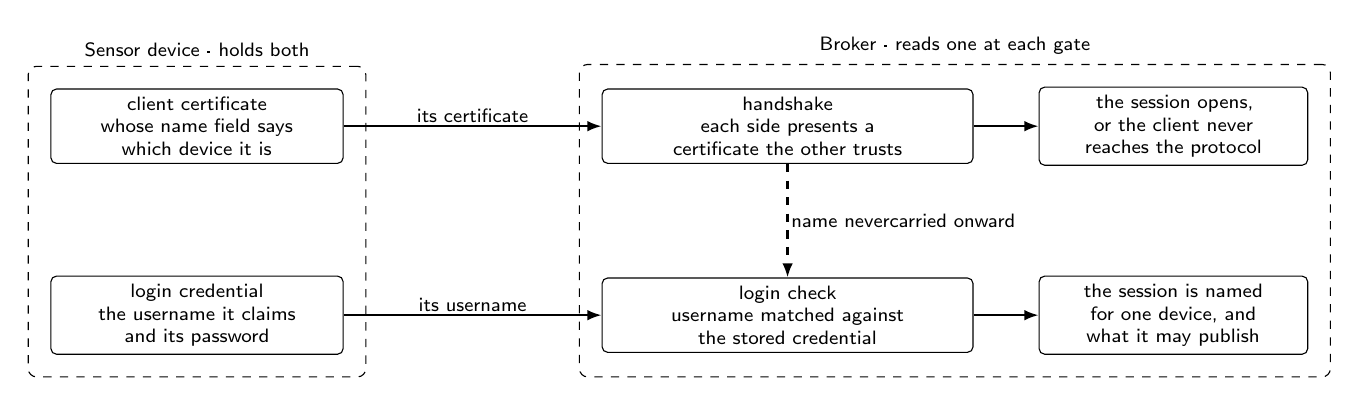
\begin{tikzpicture}[
    every node/.style={font=\scriptsize\sffamily},
    box/.style={
        draw,
        rounded corners=2pt,
        align=center,
        inner sep=3pt,
        minimum height=8mm,
        fill=white
    },
    lbl/.style={font=\scriptsize\sffamily, fill=white, inner sep=1pt}
]
    % Evidence column x=2.1 · gate column x=9.6 · verdict column x=14.5
    % Rows y=1.2 and y=-1.2; three-line boxes are 1.23cm tall, which leaves
    % the withheld link a 1.17cm band of its own between the two gates.
    \node[box, text width=3.5cm] (cert) at (2.1,1.2)
        {client certificate\\whose name field says\\which device it is};
    \node[box, text width=3.5cm] (cred) at (2.1,-1.2)
        {login credential\\the username it claims\\and its password};

    \node[box, text width=4.5cm] (hand) at (9.6,1.2)
        {handshake\\each side presents a\\certificate the other trusts};
    \node[box, text width=4.5cm] (name) at (9.6,-1.2)
        {login check\\username matched against\\the stored credential};
    \node[box, text width=3.2cm] (ver1) at (14.5,1.2)
        {the session opens,\\or the client never\\reaches the protocol};
    \node[box, text width=3.2cm] (ver2) at (14.5,-1.2)
        {the session is named\\for one device, and\\what it may publish};

    \begin{scope}[on background layer]
        \node[archhost, fit=(cert)(cred),
            label={[archlabel]above:Sensor device · holds both}]
            (dev) {};
        \node[archhost, fit=(hand)(name)(ver1)(ver2),
            label={[archlabel]above:Broker · reads one at each gate}]
            (brk) {};
    \end{scope}

    \draw[archflow] (cert.east) --
        node[lbl, above, pos=0.5] {its certificate} (hand.west);
    \draw[archflow] (cred.east) --
        node[lbl, above, pos=0.5] {its username} (name.west);
    \draw[archflow] (hand.east) -- (ver1.west);
    \draw[archflow] (name.east) -- (ver2.west);
    \draw[archflowsoft] (hand.south) --
        node[lbl, right, pos=0.5] {name never\\carried onward} (name.north);
\end{tikzpicture}%
}
\caption{Certificate and credential decide one connection separately.}
\label{fig:enc-mtls}
\end{figure}

Both shipped clients take a shortcut of their own at the same point. The
agent dials its own broker over the loopback address and verifies the
authority chain while skipping the name check
(Section~\ref{sec:gw-agent-client}); the laboratory publisher skips it too,
and additionally relaxes a verification strictness that recent releases of
the cryptographic library apply, because the authority certificates written
by earlier installations omit a usage extension that strictness looks for.
Neither weakens the plant-facing path, since the check that matters there is
a sensor verifying a broker it reaches across the network. Each is
nonetheless a place where the delivered software is looser than the protocol
allows.

What this layer cannot see is what the first row of
Table~\ref{tab:enc-questions} already records: a client that passes both
tests may send whatever it chooses on the topics it was granted, and no check
described in this section is capable of noticing what it sent. Nor is there a
floor stated for the protocol version in what gets installed, so the weakest
version both ends happen to support is the one used. Payload confidentiality
is therefore carried by the construction of the preceding section rather than
by this one, and it has to be, because the session ends at the broker and
whatever protection the session carries ends with it.

\chapter{Evaluation}
\label{ch:evaluation}

This chapter assesses the delivered platform on the
running system rather than in parts. It returns to the
numbered statements of Chapter~\ref{ch:requirements} and
to the perimeter drawn in Section~\ref{sec:threat-boundaries}:
each procedure below exists to answer one of those
statements, and each is satisfied by an observation an
operator can make on a deployment installed through the
ordinary operator path. Nothing is asserted here that
cannot be produced by repeating one of these procedures.

Two things follow from that framing and are held apart
throughout. First, a large class of claims is settled
structurally: a misuse is either refused or it is not, a
refusal is either recorded where the operator can see it
or it is lost. Those claims are established by the
procedures themselves and are reported as results. Second,
what the delivered system does not clear is reported from
the behaviour it actually has, in the final section, rather
than left for the reader to discover.

The chapter is organised as follows.

\begin{itemize}
    \item \textbf{Evaluation goals and method}
    (Section~\ref{sec:eval-method}).
    The two instruments, the procedure that drives them,
    and the rule that decides a case.
    \item \textbf{Admission and authentication}
    (Section~\ref{sec:eval-admission}).
    Whether an unregistered or wrongly credentialled
    publisher can reach the data path at all.
    \item \textbf{Protected transmission and storage}
    (Section~\ref{sec:eval-protection}).
    Whether damaged, partial, forged or unprotected
    messages are refused, and what acceptance leaves
    behind.
    \item \textbf{Monitoring and detection}
    (Section~\ref{sec:eval-monitoring}).
    Whether the operator sees the traffic, the refusals
    and the delay, and whether restriction takes effect.
    \item \textbf{Limitations}
    (Section~\ref{sec:eval-resources}).
    What the delivered system does not clear, and how far
    the procedures reach.
\end{itemize}

\section{Evaluation Goals and Method}
\label{sec:eval-method}

The system is examined with two instruments that answer
different questions, and the chapter is careful about
which is which.

Table~\ref{tab:eval-instruments} states the division. The
first instrument is the automated test suites that sit
beside each of the three code areas: the desktop
application, the operator-side service, and the gateway
runtime. Those exercise each decision in isolation,
against stand-ins for the broker, the storage service and
the remote shell, and they are the reason a claim about
ordering --- that a message is paired before it is
verified, or that a replay is recognised before anything
is opened --- can be made without a live network. Their
limitation is exactly their strength: a stand-in cannot
show what a real broker does to a session that presents a
bad certificate.

The second instrument is the one this chapter relies on.
A runner drives the laboratory sensors of
Section~\ref{sec:monitoring-fakes} through every misuse
behaviour the platform offers, one at a time, and reads
the consequence off the gateway itself. It is written
against the operator path rather than around it: misuse is
introduced by the same local interface on localhost port
9138 that the desktop application uses, and the verdict is
taken from the gateway runtime's own reporting on port
9139 --- its metrics page and its refusal summary. The
runner never edits broker configuration and never logs
into the gateway. That matters for the reading of every
result below, because it means each case demonstrates what
an operator would observe, not what a test harness can
arrange.

\begin{table}[htbp]
\centering
{\small
\begin{tabularx}{\textwidth}{@{}p{3.4cm}p{5.6cm}Y@{}}
\toprule
\textbf{Instrument} & \textbf{What it establishes} & \textbf{What it cannot establish} \\
\midrule
Automated test suites beside each component
& Each decision in isolation: the order of the checks,
the reason attached to each refusal, the capacity
refusal, the state transitions of restriction.
& Behaviour that only emerges when a real broker ends a
TLS session, drops a session's grant, or writes its own
log; and anything about the operator path that lives in
the desktop application. \\
\midrule
On-system misuse procedure over the operator path
& What a live deployment does with each misuse: the
refusal class, the counters that move, what the operator
sees, and whether the runtime survives.
& Volume behaviour and long-run drift; conclusions about
real sensor hardware; and any quantity a run was not
recorded for. \\
\bottomrule
\end{tabularx}}
\caption{The two instruments and the line between them.}
\label{tab:eval-instruments}
\end{table}

\paragraph{The procedure.}
A single case runs as follows. The laboratory unit under
test is stopped, returned to clean settings, and started
again, so that nothing from the previous case survives ---
in particular so that a unit which was made to present a
bad certificate rebuilds its transport context rather than
reusing it. Its counters and its refusal record are read.
One misuse behaviour is switched on, the unit is started,
and the run is left to settle for ten to fourteen seconds
according to how deep the check that should catch it sits.
Counters and refusal record are read again. The verdict
turns on two things: the movement in the accepted, refused
and failed counts, and the class of refusal carried by the
records that arrived in the interval. A case passes only if
a refusal of the expected class is present; a refusal
without the expected class is a failure, not a pass, since
the system would have refused for some unrelated reason.
Cases whose outcome depends on how the deployment is
configured are given a third verdict, discussed below.

Three controls hold throughout. The gateway runtime is
queried for health at the end of every case, so a case that
silently killed the runtime is a failure whatever the
traffic did. A second laboratory unit is left running clean
for the whole session, and its accepted traffic is checked
at every case: a defence that stops the attacker by also
stopping a healthy device is a failure. And after the last
case the unit under test is returned to clean settings and
required to resume accepted traffic, which is what
establishes that these defences are reversible rather than
a one-way door.

Table~\ref{tab:eval-cases} is the case set. It is stated
once here and read section by section afterwards, since the
cases differ only in where the system stops them. Each row
names one of the misuse behaviours offered in the
laboratory controls of Figure~\ref{fig:eval-simulate}; those
behaviours exist because FR-12 requires a way to exercise
admission, protected transmission and misuse patterns
without physical hardware, so the instrument of this
chapter is itself one of the requirements of
Chapter~\ref{ch:requirements}.

\appshot{UI-to-simulate-maclious-behavior-for-test-sensor.png}
    {The misuse behaviours offered against a laboratory sensor}
    {fig:eval-simulate}

Twelve of the eighteen cases are expected to be refused.
Four are marked conditional, and their conditionality is
not a weakness of the procedure but the point of them: they
are the places where Chapter~\ref{ch:encryption} showed a
check to be contingent on the profile in force or on what
the operator registered, and a procedure that reported them
as unconditional passes would be reporting something the
system does not do. Two are expected to be accepted, one of
them because accepting is the designed compatibility
behaviour.

\begin{longtable}{@{}p{5.2cm}p{3.0cm}p{3.2cm}p{2.6cm}@{}}
\caption{The misuse case set, by the stage that stops it.}
\label{tab:eval-cases}\\
\toprule
\textbf{Misuse introduced} & \textbf{Stage that stops it} &
\textbf{Verdict} & \textbf{Answers} \\
\midrule
\endfirsthead
\caption[]{The misuse case set, by the stage that stops it
(continued).}\\
\toprule
\textbf{Misuse introduced} & \textbf{Stage that stops it} &
\textbf{Verdict} & \textbf{Answers} \\
\midrule
\endhead
\bottomrule
\endlastfoot
Client certificate withheld & Transport handshake & Refused & FR-2 \\
\addlinespace
Certificate from another device & Transport handshake & Refused & FR-2 \\
\addlinespace
Wrong password & Broker admission & Refused & FR-1, FR-2 \\
\addlinespace
Publish on another device's topic & Session's grant & Refused & FR-2 \\
\addlinespace
Message sent in the clear & Agent, before opening & Refused & FR-3 \\
\addlinespace
Wrapper that will not open & Agent, opening & Refused & FR-3 \\
\addlinespace
Key half published alone & Agent, pairing halves & Refused & FR-3 \\
\addlinespace
Data half published alone & Agent, pairing halves & Refused & FR-3 \\
\addlinespace
Binding stamp altered on the key half & Agent, binding check & Refused & FR-3 \\
\addlinespace
Binding stamp altered on the data half & Agent, binding check & Refused & FR-3 \\
\addlinespace
Halves taken from two messages & Agent, binding check & Refused & FR-3 \\
\addlinespace
Day stamp outside the accepted window & Agent, day check & Conditional & FR-3 \\
\addlinespace
Day material withheld & Envelope profile & Conditional & FR-3 \\
\addlinespace
Field the shape requires left out & Shape check & Conditional & FR-3 \\
\addlinespace
Field given the wrong type & Shape check & Conditional & FR-3 \\
\addlinespace
Field added beyond the shape & Shape check & Accepted unless closed & FR-3 \\
\addlinespace
Schema the device was not given & Shape check & Refused & FR-3 \\
\addlinespace
Legacy wrapper from an older device & Compatibility path & Accepted by design & FR-3, NFR-5 \\
\end{longtable}

\section{Admission and Authentication}
\label{sec:eval-admission}

The first four rows of Table~\ref{tab:eval-cases} are
settled before any payload is read, and they separate
cleanly because the broker decides them at two different
moments.

The first two --- a session that presents no client
certificate, and one that presents a certificate the
gateway's authority did not issue --- are decided while the
transport is being established. No session exists
afterwards, so nothing reaches the topic grant and nothing
reaches the gateway runtime's payload-stage counters. The
observed signature of these two cases is therefore precise:
the unit's accepted count does not move, and the only trace
is the entry the runtime extracts by following the broker's
own log, which the installation keeps at its most verbose
level for this reason (Section~\ref{sec:gw-broker-decisions}).
Were that setting lowered, these two cases would still be
refused but would become invisible in the operator's view of
refusals --- a dependence worth stating, because it means the
visibility of door-stage refusals rests on a configuration
choice rather than on the refusal itself.

The third case, a wrong password, is the same in kind: the
session is not admitted. The fourth is different in an
important way. A device that authenticates correctly and
then publishes on a topic it holds no grant for has already
been let in; it is refused by the permissions attached to
its own session (Section~\ref{sec:gw-broker-decisions}). The
consequence is that this case, unlike the first three,
produces a refusal with a session behind it: a delivery the
broker was asked to accept and declined, recorded with the
address it came from. That difference matters twice over. It
is the reason the two-stage design is worth having --- an
intruder who has obtained a valid credential still cannot
write where it is not permitted --- and it is also the
reason only some refusals can feed the automatic
restriction of Section~\ref{sec:eval-monitoring}: a refusal
that never established a session may carry no address the
restriction control could act on.

Across all four cases the clean laboratory unit keeps
connecting and publishing. Enforcement is selective, which
is what makes the first four rows evidence for FR-1 and
FR-2 rather than evidence for a blunt instrument: the
gateway refuses the wrong credential, the wrong certificate
and the wrong topic while accepting the right ones on the
same port at the same moment. What these cases do not
establish is that a certificate and a credential belong to
one device; that question is answered by construction rather
than by measurement, and it is returned to in
Section~\ref{sec:eval-resources}.

\section{Protected Transmission and Storage}
\label{sec:eval-protection}

The remaining fourteen rows are decided inside the gateway,
after the transport has been terminated and a session has
already been accepted. That difference is visible in the
readings: where the door-stage cases left the runtime's
counters untouched, every one of these moves the runtime's
own refused count and leaves a record carrying the address
the publication came from (Section~\ref{sec:gw-in-signals}).

\paragraph{The two halves.}
A protected message arrives as two publications on two
topics, so a party able to drop one of them can test whether
the gateway treats an incomplete message as a smaller
message. It does not. Publishing only the key half, or only
the data half, is refused with a reason that names which
half arrived, and the accepted count does not move. The
pairing rule is what makes a dropped half a refusal instead
of a silent gap, and it is worth noting what the procedure
cannot see: it cannot show \emph{why} the other half is
missing, only that its absence was not mistaken for a
complete message.

\paragraph{The binding stamp.}
Three cases test the stamp that ties the halves together,
and they are the strongest results in the set. Because one
stamp covers the union of the fields in both halves and is
written identically into both of them, altering either half
invalidates it --- which is why the case set carries two
near-identical rows, one tampering with each half, and why
neither is sufficient on its own. Substituting one half's
message identifier for another's is caught the same way, as
a mismatch between the halves rather than as a decryption
failure.

The order in which these are caught matters more than that
they are caught. The stamp is recomputed from the declared
fields of the two halves before any key is unwrapped, so a
tampered message is refused without the gateway performing
the cryptographic work that tampering is meant to provoke,
and --- more importantly for the argument of
Chapter~\ref{ch:encryption} --- without any plaintext ever
having existed to be mistakenly used. The refusal of a
tampered message and the refusal of a message that simply
cannot be opened are therefore distinguishable in the
record, which is what lets the operator tell tampering from
a device with the wrong material.

\paragraph{The four conditional cases.}
These are reported as conditional because the system's
answer genuinely depends on how the deployment is
configured, and each conditional row names the condition.

A day stamp outside the accepted window is refused, and the
laboratory substitution uses a date decades past, so this
case stops in practice. What the row records as conditional
is the window itself: it admits today together with one day
either side, so a faithfully built message from yesterday is
admitted by design rather than by oversight. Whether such a
replay is stopped therefore rests on the replay check
discussed in Section~\ref{sec:eval-resources}, not on the
day rule.

Withholding the day material has no effect on a deployment
using the pre-shared-secret profile, because that profile
never consults day material; the case is recorded as not
applicable rather than as a pass, which is the honest
outcome and the reason the procedure keeps a third verdict
instead of forcing every case to be a yes or a no.

The two shape cases that concern a required field and a
field of the wrong type stop only where the operator has
registered a shape that requires the field or declares the
type. This is not a hedge: the shape registered for a device
at registration is the whole content of the check, and the
shape registered by default declares nothing about which
fields must be present. A procedure that reported these two
rows as passes on a default registration would be measuring
the operator's configuration, not the gateway.

\paragraph{What the shape layer does guarantee.}
The one shape-stage refusal that is unconditional is the
last row of its group: naming a shape that was never
registered is refused, because for any name other than the
default the gateway requires a registered shape behind it.
It is precisely the default name that is honoured with
nothing registered behind it. Read together with the two
conditional rows above, that is the honest statement of what
this layer contributes: the shape check is exactly as strong
as the shapes the operator registered, and the procedure
shows both halves of that sentence.

\paragraph{The two accepted cases.}
An extra field beyond the registered shape is accepted
unless the operator closed the shape against extras, which
is a policy the operator holds rather than a property of the
gateway. The older protected form sent by a device that
predates the envelope design is accepted while the operator
has not made the envelope form mandatory, and this is the
one case whose expected verdict is a refusal of nothing at
all. It is included because the compatibility concession is
part of the delivered system and a reader is entitled to see
it exercised. It is not accepted silently: the count of
messages admitted through the older form is reported
separately from the count admitted through the envelope
form, so the concession is visible as a number the operator
can watch rather than inferred from configuration.

\paragraph{What acceptance leaves behind.}
FR-4 and NFR-5 are both statements about the accepted path,
and the clean control unit settles them. For every accepted
message two things appear: a line in the sensor data log on
the gateway, and a record on the device's own storage topic,
each with its own counter that rises in step with the
accepted count. The second half of NFR-5 is settled by the
cases above rather than by this one: in every refused case
neither of those two counters moved, so a failed attempt
contributed to refusal signalling and not to accepted
output. Nothing in the accepted output had to be trusted to
have been checked --- the readings show that it was.

\section{Monitoring and Detection}
\label{sec:eval-monitoring}

FR-7, FR-8 and FR-9 are claims about what the operator can
see, so they are evaluated by asking what the gateway
reports and whether the report is adequate to the question
being asked. Table~\ref{tab:eval-observability} pairs each
question a reader of this chapter might pose with the
reading that answers it. Every row is obtained from the
gateway's own reporting rather than from instrumentation
added for the evaluation, which is what makes the pairings
reproducible.

\begin{table}[htbp]
\centering
{\small
\begin{tabularx}{\textwidth}{@{}p{5.6cm}Y@{}}
\toprule
\textbf{Question} & \textbf{What the gateway reports} \\
\midrule
Which part of the runtime is alive?
& A liveness reading for the process itself, for each of
its working roles, and for the broker and storage service it
depends on --- so a runtime that is up but cut off from
storage reads differently from a healthy one. \\
\addlinespace
How much has been accepted, and how much refused?
& A gateway-wide refusal total, and for each device a pair
of accepted and refused counts labelled with that device and
its storage topic. \\
\addlinespace
Why was it refused?
& The refusal record served over the same surface, each
entry carrying the class of refusal, the device and an
arrival time; and the shipped activity lines that feed the
operator's view of transmissions. \\
\addlinespace
How long does the gateway hold a message?
& A per-device processing delay measured from receipt at the
broker to produce at storage, with its running total and a
sample count, so an average can be recovered but no single
reading is taken as typical. \\
\addlinespace
Is the compatibility concession in use?
& A count reserved to messages admitted through the older
protected form, separate from the envelope count. \\
\addlinespace
Is anything actually reaching the operator?
& The count of shipped lines, and the storage produce counts
split into those that succeeded and those that did not. \\
\addlinespace
What is each piece costing?
& Cumulative processor time and resident memory for the
runtime, the broker and the storage service individually. \\
\addlinespace
Is the host itself healthy?
& Load, memory and swap, filesystem size and availability,
traffic per network interface, running and blocked process
counts, and a hardware temperature reading. \\
\bottomrule
\end{tabularx}}
\caption{What the gateway reports, against the question each reading answers.}
\label{tab:eval-observability}
\end{table}

Two observations follow from the table rather than from any
single row. The first is that the readings are sufficient to
reconstruct the case set after the fact: because refusals
carry both a class and an arrival time, and because the
per-device counts are labelled with the device, an
evaluation can attribute a refusal to the case that caused
it without pausing the run to inspect anything. That is what
allowed the verdict rule of Section~\ref{sec:eval-method} to
insist on the expected refusal class rather than on a count
merely moving. The second is that delay is reported as a last
value with a running total and a sample count, which
supports a mean over a window but not a claim about
worst-case latency; that distinction is carried into the
final section of this chapter.

\paragraph{The manual control.}
FR-10 --- withholding and restoring a device's publish
rights --- is exercised through the operator controls
described in Chapter~\ref{ch:monitoring}, and the same
readings settle it: while a device is withheld its accepted
count is flat and its refused count rises if it keeps
publishing, and both resume when the right is restored. The
control is therefore observable in the same place as the
misuse cases, which is a property of the design rather than
an artefact of the procedure.

\paragraph{Repeated misuse and automatic restriction.}
FR-11 cannot be settled by the case set, and the reason is
instructive. The case set introduces one behaviour at a time
and waits for a verdict, whereas the restriction is a
per-device policy that counts refusals inside a sliding
window --- ten within five minutes unless the operator sets
it otherwise, with a floor of one and a window no shorter
than a minute --- and it stays off until the operator enables
it for a device. A procedure that produces one refusal per
case does not reach a threshold of ten.

The procedure for FR-11 is therefore separate. The policy is
enabled for one laboratory unit, that unit is driven to
produce invalid messages continuously rather than singly, and
the count is watched within the window. When it trips, two
readings change: traffic from that source is dropped at the
gateway's own firewall by a privileged helper, and the
restriction state records the device, the count and the
window that produced it. Clearing the restriction through the
operator path restores traffic, which is the part of FR-11
that a detection claim usually omits and that this requirement
states explicitly.

Two conditions attach to that result. Only refusals carrying
a usable host address contribute to the count: an address
that is absent, local to the gateway itself, or otherwise not
a host cannot be dropped, so the door-stage cases of the
preceding section largely do not feed the restriction at
all. The mechanism that notices the most common misuse is
therefore not the mechanism that responds to it, and an
evaluation that measured only refusals would overstate the
reach of the response. The second condition is that the
policy counts refusals, not intent, so a device that is
merely misconfigured reaches the same threshold as one that
is attacking; what keeps that consequence manageable is that
the operator can inspect the class of refusal before the
count is reached.

\section{Limitations}
\label{sec:eval-resources}
The limits below are stated plainly because an evaluation
that listed only successes would be worth little. Each was
established by reading the delivered behaviour, not by
experiment failing to produce a result.

\begin{itemize}
    \item \textbf{A certificate is not bound to a credential.}
    The broker verifies that a certificate was issued by the
    gateway's authority and, separately, that a username and
    password are valid; nothing ties the two to one device.
    Material from two devices connects as the owner of the
    credential, so the transport proves possession of
    deployment material rather than the identity of a device.
    \item \textbf{An issued certificate cannot be retired
    alone.} There is no revocation list and no per-device
    withdrawal of a certificate. Withdrawing a device works
    through its credential and its topic grant, which is
    effective; retiring the certificate itself means rotating
    the authority, which invalidates every issued
    certificate at once.
    \item \textbf{The compatibility form protects little.}
    The older wrapper is authenticated but carries the key
    that opens it alongside the ciphertext, so accepting it
    admits a message that is effectively unprotected. This is
    why the concession is counted separately, and why the
    envelope form can be made mandatory by the operator.
    \item \textbf{The shape layer inherits its strength from
    the operator.} The default shape declares nothing, so
    with default registrations the shape check accepts almost
    any plaintext; only the shapes actually registered do
    work.
    \item \textbf{Replay protection is not durable.} Repeated
    identifiers are recognised from an in-memory record of a
    few thousand entries, trimmed when full and lost when the
    runtime restarts, while the day window admits today
    together with one day either side. A faithfully built
    message replayed inside that window after a restart is
    therefore admitted.
    \item \textbf{Stored records are not forward-secret.}
    Day material is never discarded, and on the
    pre-shared-secret profile the daily key is derived from a
    registration secret that does not change. The gateway
    also holds each device's material in readable form. A
    later compromise of a device, or of the gateway itself,
    therefore opens traffic that was captured and stored
    earlier.
    \item \textbf{Restriction depends on an address and on
    counting.} It can only act on a refusal that carries a
    usable host address, and it counts refusals rather than
    malice, so the worst-configured innocent device is
    restricted alongside an attacker.
    \item \textbf{The operator-facing surfaces assume a
    trusted network.} Neither the gateway's reporting surface
    nor the storage listener the dashboard reads authenticates
    the machine asking; both trust the network they sit on.
    The privileged path out of the operator PC rests on one
    credential per gateway, held in the keyring. NFR-9 states
    the network assumption explicitly, and it holds only
    inside the plant or laboratory network the design is
    written for; the protections described here do not
    transfer to a deployment exposed beyond it.
    \item \textbf{The scope of these procedures.} Each case
    introduces one behaviour, so combined or staged attacks
    are untested; there is no sustained-volume or long-run
    soak, so drift and retention behaviour over weeks are
    unmeasured; no physical sensor hardware was used; the
    laboratory units run on the gateway itself rather than on
    separate hardware; and the delay figures support a mean,
    not a percentile claim.
\end{itemize}

What the procedures do establish is narrower but solid: on a
deployment installed by the ordinary operator path, every
misuse that the design claims to stop is stopped, each
refusal is refused at the stage that ought to catch it and is
recorded where the operator can see it, the refusals do not
disturb a healthy device, and the gateway that refuses them
survives and remains inspectable. The consequences of the
limits above, and what would be worth doing about them, are
taken up in Chapter~\ref{ch:conclusion}.

\chapter{Conclusion and Future Work}
\label{ch:conclusion}

This thesis set out to operate a secure gateway end to end
for edge telemetry: to admit only registered devices, to
keep the inbound path protected after the transport is
terminated, to make refusal visible to the operator, and to
give that operator a response that can be undone. This
chapter states what the delivered system established on
those terms, what the work contributed beyond the
individual parts, and which directions follow from what the
system did not settle.

\section{Summary}

The problem was an admission problem before it was a
cryptography problem. A factory broker that accepts any
client holding a password gives an unknown device a path
into the internal data path that operators depend on, and a
payload that survives transport termination unprotected
gives that device a voice inside the path. The delivered
system answers it with a gateway that decides, for every
message, whether the device is admitted, whether the message
is protected and shaped as its registration declared, and
what the operator is told when either fails.

Two runtimes carry that decision. On the operator PC, the
monitoring application provisions a gateway over an ordinary
remote session, registers and unregisters devices, runs the
local metrics and log stack, and offers day to day what an
operator needs: health, per-device transmission, refusals
with the class of each, publish rights, and restriction. On
the edge host the agent sits beside the broker and the
storage service: it verifies what the transport established,
opens the application-layer protection, checks the declared
shape, and forwards only what passes to the local log and
the device's own storage topic. What fails is refused at the
stage that owns the check and recorded with a class and an
arrival time, which is what turns a refusal from a line in a
broker log into something an operator can act on.

The assessment treated the system as one object. An
eighteen-case misuse set was driven over the operator path
against a deployment installed by that same path, one
behaviour at a time, with the verdict taken from what the
gateway itself reports. On that evidence every misuse the
design claims to stop was stopped, each at the stage that
ought to catch it; the refusals were visible without
disturbing a healthy device on the same broker; and the unit
that produced them was returned to clean settings and
resumed accepted traffic, which is what establishes that the
response is reversible rather than a one-way door. Four
cases were reported as conditional because the answer
genuinely depends on the protection profile in force or on
what the operator registered, and reporting those as
unconditional passes would have claimed a behaviour the
system does not have. Footprint and capacity were bounded by
policy rather than by measurement: retention is budgeted
against the host's disk at registration, and a registration
that cannot be budgeted is refused, so growth stops at a
decision rather than at a full device.

The limits in Section~\ref{sec:eval-resources} belong to the
same result. Transport material proves possession of
deployment material rather than the identity of a device,
and once issued it cannot be withdrawn on its own; the
compatibility form of the message wrapper is authenticated
but carries the key that opens it; the shape layer does work
only on the shapes an operator actually registers; the
replay record is held in memory and the day window is wide,
so a faithfully built replay after a restart is admitted;
stored records are not forward-secret; restriction needs a
usable source address and counts refusals rather than intent;
and the reporting surfaces trust the network they sit on.
These are what an honest assessment of a modest-host,
trusted-LAN design has to concede. The two identity limits
and the manual half of the delivery path return below as
work rather than being argued away.

\section{Contributions}

The contribution is a system rather than four components,
and the parts are worth naming separately only because the
function exists when they are joined.

\begin{itemize}
    \item \textbf{A complete inbound security path on one
    edge host.}
    Registration binds a device identity to its transport
    credentials, its topic permissions, its certificate and
    its storage topic, so admission is one decision with one
    owner. Protection is layered above that decision ---
    transport, an application-layer envelope, a check of the
    message against the declared shape --- and each layer
    refuses in its own name, which is what makes a refusal
    diagnosable rather than merely observed.

    \item \textbf{Detection joined to the operator's view.}
    Denied connections and invalid messages reach the same
    surface as accepted traffic, counted, classed and
    attributed to a device, so misuse is read against the
    healthy traffic it sits among instead of in a separate
    log the operator has to know to go and find.

    \item \textbf{A reversible response.}
    Blocking publish rights, restricting a source at the
    firewall after a configurable count inside a window, and
    clearing that restriction are operator actions with
    visible state; the assessment exercised them by producing
    misuse and then restoring the unit to normal operation.

    \item \textbf{A route from source to a usable package.}
    The operator application is built and published by a
    pipeline rather than rebuilt on a workstation, and a
    gateway is provisioned from the application rather than
    by hand-editing broker configuration --- which is what
    makes the functions above operable without
    reconstructing the system from research scripts.

    \item \textbf{An assessment that keeps measured and
    unmeasured apart.}
    A reproducible misuse case set run over the operator path,
    reported by the stage that produced each verdict, with
    conditional outcomes named as conditional and quantities
    that were never recorded left out rather than filled in.
\end{itemize}

\section{Future Work}

Three directions follow from the delivered system: one
extends what it detects, one extends how it reaches an
operator, and one closes the identity gap the assessment
could not settle. None of them is a change of subject.

\subsection{A learned detector beside the rule set}

Detection in the delivered system is rule-shaped. A transport
denial is a denial, an invalid message carries the class of
its failure, and a device is restricted after a configurable
count of refusals inside a window. That is the right shape
for a claim an operator can audit, since every restriction
traces back to counted refusals, but it is blind to anything
the rules do not name; and, as Section~\ref{sec:eval-resources}
observes, it counts refusals rather than intent, so the
worst-configured innocent device reaches the same threshold
as one that is probing the gateway.

A learned detector is the natural second stage, and it is
the work that Chapter~\ref{ch:requirements} deliberately left
outside the delivered scope. The platform already records the
features such a detector needs: per-device accepted and
refused counts, the class of each refusal, arrival times, and
the measured holding time per message. A classifier over
sliding windows of those features could separate a
misconfigured sensor from a probing one, which is the
distinction a threshold cannot draw, and could rank devices
for the operator's attention before any threshold is reached.
Gradient-boosted trees are a plausible first choice at this
feature scale and on this class of host \cite{lightgbm}.
Labelled MQTT traffic carrying both benign and malicious
scenarios has been published for exactly this
purpose~\cite{mqttset}, and learned detectors over
network-level statistics of constrained IoT devices are
already well established~\cite{nbaiot}.

Two conditions belong to that work. First, the evidence in
this thesis is not training data: eighteen misuse behaviours,
produced one at a time against laboratory units on the
gateway itself, say nothing about the distribution of normal
plant traffic, so the useful next step is a labelled
collection from a real deployment rather than a model.
Second, a learned score has to sit in front of the response
rather than behind it: its verdict should raise an operator
prompt beside the rule-based restriction it annotates, not
replace the rule as the trigger for a firewall drop. A false
positive that silently cuts a healthy production sensor is
the specific harm the delivered rule set is built to avoid,
and a model whose error rate on plant traffic is unknown
should not be handed that authority.

\subsection{Automatic delivery of the operator application}

The build half of delivery is already automated: a change on
a packaging branch rebuilds that platform's package and
replaces it on one standing release with checksums beside it,
so an operator is always pointed at the same address for the
current build (Section~\ref{sec:arch-delivery}). The install
half is not. The operator has to
learn that a new build exists, fetch it, and run it --- and
because the interface is embedded when the package is built,
an interface change reaches a plant only when somebody
reinstalls. For an operator who is not in the business of
distributing software, that gap is where updates actually
fail.

The next step is an update path inside the application:
consult the release the installation came from, compare its
build against the one running, offer the difference to the
operator, and verify the package against the checksum and
signature the packaging path already produces before anything
is applied. Three properties matter more than the mechanism.
Available should stay separate from accepted, so a site can
defer an update across a production campaign or a shutdown
window. The update should preserve what an installation owns
--- its registry of gateways, the credentials held in the
system keyring, the local metrics and log store, and the
dashboard certificate the operator chose to trust --- since
losing those is what makes an update feel like a risk rather
than a routine act. And the same channel should eventually
carry the agent on the gateway, which today is replaced by
reinstalling it; a fleet of gateways that cannot be brought
forward without a session on each host is the same
operational problem one floor further out.

Signing belongs to this work rather than following it, and is
the reason the direction is not merely convenient. An
automatic update path is a route by which anyone who can
reach the release can run code on an operator's PC, so
verification is the design and not a detail: material that
is unsigned or wrongly signed should be refused outright
rather than offered with a warning.

\subsection{Per-device identity that can be withdrawn}

The most consequential gap is the one the transport cannot
close today. The broker checks that a certificate was issued
by the gateway's authority and, separately, that a username
and password are valid; nothing ties the two to the same
device, so one device's material presented with another
device's credential connects as the owner of that credential.
The transport therefore proves possession of deployment
material, which is weaker than the admission requirement's
wording invites a reader to assume. Withdrawal has the same
shape: a credential and a topic grant can be taken away, a
certificate cannot, so retiring a single device means
rotating the authority and invalidating the material of every
device at once.

Closing it means making the certificate carry the identity
the broker is already believed to be checking --- naming the
device in the material and requiring the session to present
the pair belonging to the device it claims --- and making
withdrawal an ordinary action. Short-lived material that the
application renews, and simply stops renewing when a device
is retired, is the cleaner route; a revocation state the
broker consults before accepting a session is the alternative
the standard profile for this material describes
\cite{x509}. The operational shape already exists: the
application issues, stores and renews device material, and
already knows how to withdraw a device's publish rights. What
is missing is that the two halves must be treated as one
claim rather than two, and that some record has to survive a
restart to say which device is no longer trusted. Until then,
the narrower claim this thesis makes is the correct one, and a
deployment that needs per-device revocation on the wire has
only authority rotation available and should plan for its
blast radius.

The limits not taken up above are open for a reason worth
stating. A replay record held in memory and a day window a
day wide on either side are the price of a runtime that
restarts cleanly on a modest host; stored traffic that a
later compromise can open is the price of keeping the
material that decrypts it; reporting surfaces that trust
their network are NFR-9's assumption stated where it bites.
Each of those changes only if the deployment the system was
written for changes with it, and saying so is the last claim
this chapter makes.

% =========================================================
% BIBLIOGRAPHY — one entry per source cited in the text
% =========================================================
\begin{thebibliography}{99}

\bibitem{mqtt}
OASIS,
\emph{MQTT Version 5.0},
OASIS Standard, 7 March 2019.
\url{https://docs.oasis-open.org/mqtt/mqtt/v5.0/os/mqtt-v5.0-os.html}

\bibitem{tls}
E. Rescorla,
\emph{The Transport Layer Security (TLS) Protocol Version 1.3},
RFC 8446, 2018.
\url{https://www.rfc-editor.org/rfc/rfc8446}

\bibitem{x509}
D. Cooper, S. Santesson, S. Farrell, S. Boeyen,
R. Housley, and W. Polk,
\emph{Internet X.509 Public Key Infrastructure Certificate
and Certificate Revocation List (CRL) Profile},
RFC 5280, 2008.
\url{https://www.rfc-editor.org/rfc/rfc5280}

\bibitem{mqttsurvey}
B. Mishra and A. Kertesz,
``The Use of MQTT in M2M and IoT Systems: A Survey,''
\emph{IEEE Access}, vol. 8, pp. 201071--201086, 2020.
\url{https://doi.org/10.1109/ACCESS.2020.3035849}

\bibitem{sre}
B. Beyer, C. Jones, J. Petoff, and N. R. Murphy,
\emph{Site Reliability Engineering: How Google Runs
Production Systems}.
O'Reilly Media, 2016.
\url{https://sre.google/sre-book/table-of-contents/}

\bibitem{loganalysis}
J. Ma, Y. Liu, H. Wan, and G. Sun,
``Automatic Parsing and Utilization of System Log Features
in Log Analysis: A Survey,''
\emph{Applied Sciences}, vol. 13, no. 8, art. 4930, 2023.
\url{https://doi.org/10.3390/app13084930}

\bibitem{lightgbm}
G. Ke, Q. Meng, T. Finley, T. Wang, W. Chen,
W. Ma, Q. Ye, and T.-Y. Liu,
``LightGBM: A Highly Efficient Gradient Boosting Decision Tree,''
\emph{Advances in Neural Information Processing Systems},
vol. 30, 2017.
\url{https://proceedings.neurips.cc/paper/6907-lightgbm-a-highly-efficient-gradient-boosting-decision-tree.pdf}

\bibitem{mqttset}
I. Vaccari, G. Chiola, M. Aiello, M. Mongelli,
and E. Cambiaso,
``MQTTset, a New Dataset for Machine Learning
Techniques on MQTT,''
\emph{Sensors}, vol. 20, no. 22,
article 6578, 2020.
\url{https://doi.org/10.3390/s20226578}

\bibitem{nbaiot}
Y. Meidan, M. Bohadana, Y. Mathov, Y. Mirsky,
A. Shabtai, D. Breitenbacher, and Y. Elovici,
``N-BaIoT---Network-Based Detection of IoT Botnet Attacks
Using Deep Autoencoders,''
\emph{IEEE Pervasive Computing}, vol. 17, no. 3,
pp. 12--22, 2018.
\url{https://doi.org/10.1109/MPRV.2018.03367731}

\end{thebibliography}

\end{document}